\documentclass[twoside,notitlepage,11pt]{report}
%\usepackage{a4paper}
\usepackage{graphicx}
\usepackage{psfrag}
\usepackage{amsfonts}
\usepackage{amsmath}
\usepackage{amsbsy}
\usepackage{verbatimfile}
\usepackage{fancyhdr}
\usepackage{pstricks,pst-node}
% The next rawfonts package one is used in the ``datablad''.
\usepackage[only,egtrm]{rawfonts}
% Handle sorting in reference list
\usepackage{citesort}
% Create an index table
\usepackage{makeidx}

\newcommand{\smallverbatimfile}[1]{{\footnotesize\verbatimfile{#1}}}
\newcommand{\component}[5]{\begin{tabular}{|lp{0.7\textwidth}|}\hline {\bf Name:} & #1 \\ \hline {\bf Author:} & #2 \\ \hline {\bf Input parameters} & #3 \\ \hline {\bf Optional parameters} & #4 \\ \hline {\bf Notes} & #5 \\ \hline \end{tabular} \\ \noindent }

\def\reportnum{Ris{\o}--R--1538(rev.ed.)(EN)}

%\oddsidemargin 0cm
%\evensidemargin 0cm
\addtolength{\hoffset}{-1.4cm}
\topmargin 0cm
\textwidth 15cm
\textheight 22cm
\addtolength{\footskip}{1.6pt}
\addtolength{\headheight}{1.6pt}

\pagestyle{fancy}
\fancyhf{}
\fancyfoot[LE,RO]{\thepage}
\fancyfoot[LO,RE]{\reportnum}
\renewcommand{\headrulewidth}{0pt}
\renewcommand{\footrulewidth}{0pt}

\fancypagestyle{plain}{%
\fancyhf{}
\fancyfoot[LE,RO]{\thepage}
\fancyfoot[RE,LO]{\reportnum}
\renewcommand{\headrulewidth}{0pt}
\renewcommand{\footrulewidth}{0pt}}

\newcommand{\MCX}{{McXtrace}}
\newcommand{\MCS}{{McStas}}
\newcommand{\version}{{1.0\_rc1}}
\newcommand{\reldate}{{Mar, 2011}}
\newcommand{\Ombold}{\mbox{\boldmath $\Omega$}}

\newcommand{\NBIlong}{Niels Bohr Institute, Univeristy of Copenhagen, Copenhagen, Denmark}
\newcommand{\Lifelong}{Faculty for Life Sciences, University of Copenhagen, Copenhagen, Denmark}


% enable index generation
\makeindex

%\title{Component manual\\ to the neutron ray-tracing package
% \MCX ,\\ version \version}
%\author{Kim Lefmann, Peter Kj\ae r Willendrup, and Kristian Nielsen, \\
% Materials Research Department, \\
% Ris\o\ National Laboratory, 4000 Roskilde, Denmark;\\
% Emmanuel Farhi and Klaus Lieutenant \\ ILL, Grenoble, France}
%\date{\reldate \\[2\baselineskip]
%\begin{center}
%  \includegraphics[width=4.5in]{figures/vanadium-surf-2.eps}
%\end{center}
%
\includegraphics[width=0.45\myheight]{risoe-logo.eps}%
%}

% The following definitions relate to the appendix on polarisation
\usepackage[dvips]{epsfig}
\usepackage{amsmath}
\parindent=0pt

\newcommand{\kappaB}{\mbox{\boldmath $\kappa$}}
\newcommand{\etaB}{\mbox{\boldmath $\eta$}}
\newcommand{\alphaB}{\mbox{\boldmath $\alpha$}}
\newcommand{\sigmaB}{\mbox{\boldmath $\sigma$}}
\newcommand{\tauB}{\mbox{\boldmath $\sigma$}}
\newcommand{\muB}{\mbox{\boldmath $\mu$}}

\def\nup{n_\uparrow}
\def\nd{n_\downarrow}

\def\Pu{P(\uparrow)}
\def\Pd{P(\downarrow)}
\def\Tu{T_\uparrow}
\def\Td{T_\downarrow}
\def\Ru{R_\uparrow}
\def\Rd{R_\downarrow}

\def\dB{\mathbf{d}}
\def\fB{\mathbf{f}}
\def\lB{\mathbf{l}}
\def\mB{\mathbf{m}}
\def\nB{\mathbf{n}}
\def\sB{\mathbf{s}}

\def\BB{\mathbf{B}}
\def\PB{\mathbf{P}}
\def\RB{\mathbf{R}}
\def\SB{\mathbf{S}}

\def\nTB{\mathbf{\tilde{n}}}

\def\Q{\mathbf{\kappaB}}
\def\tP{\mathbf{\tilde{P}}}
\def\tQ{\mathbf{\tilde{\Q}}}
\def\tN{\mathbf{\tilde{\etaB}}}
\def\FN{F_N(\Q)}
\def\FM{F_M(\Q)}
\def\ru{r_\uparrow}
\def\rd{r_\downarrow}

\def\so{\mathbf{\hat{s}}}
\def\rhoo{\hat{\rho}}
\def\betao{\hat{\beta}}
\def\alphao{\hat{\alphaB}}
\def\sigmao{\hat{\sigmaB}}
\def\sigmaH{\hat{\sigma}}
\def\muno{\mathbf{\hat{\muB}_n}}
\def\vo{\hat{V}_\BB}
\def\Io{\mathbf{\hat{I}}}

\def\madsq{|\overline{A}_d|^2}
\def\sqmad{\overline{|A_d|^2}}
\def\bd{\overline{|B_d|^2}I_d(I_d+1)}

\def\chiU{\chi_\uparrow}
\def\chiD{\chi_\downarrow}

\begin{document}

%\maketitle
% Emacs settings: -*-mode: latex; TeX-master: "manual.tex"; -*-

\begingroup                     % Make all definitions local.

%
% This was modified from risoe.sty, <2 Aug 95>
%
\catcode`\@=11
\def\@magscale#1{ scaled \magstep#1 }
\font\frtnbf = cmb10 \@magscale2
\font\twfvbf = cmbx10   \@magscale5 % extended bold
\def\maketitle{\par
 \begingroup
 \def\thefootnote{\fnsymbol{footnote}}
 \def\@makefnmark{\hbox to 0pt{$^{\@thefnmark}$\hss}}
 \if@twocolumn
 \twocolumn[\@maketitle]
 \else \newpage
 \global\@topnum\z@ \@maketitle \fi\thispagestyle{empty}\@thanks\newpage
 \endgroup
 \setcounter{footnote}{0}
 \let\maketitle\relax
 \let\@maketitle\relax
 \gdef\@thanks{}\gdef\@author{}\gdef\@title{}\let\thanks\relax}
\def\@maketitle{\newpage \baselineskip 30dd \mbox{}
 \marginpar{{\frtnbf \hfill \llap{\mbox{\reportnum \reportlan\qquad\qquad}}}}
% \par\noindent\mbox{
\includegraphics[height=1.5cm]{figures/risoe-logo.eps}\hspace{2mm}
\includegraphics[height=1.5cm]{figures/DTU_logo.ps}} \par
 \par\noindent\mbox{
\includegraphics[height=2.5cm]{figures/ku-nbi-logo.eps}\hspace{2cm}
\includegraphics[height=1cm]{figures/risoe-logo.eps}\hspace{2cm}
\includegraphics[height=2.5cm]{figures/DTU_logo.ps}} \par
 \vskip 1.5cm
 {\twfvbf \noindent \@title \par} \vskip 20dd \baselineskip 16dd
 {\frtnbf\noindent\@author \par} 
 \vskip 3.0cm
 \begin{center}
%     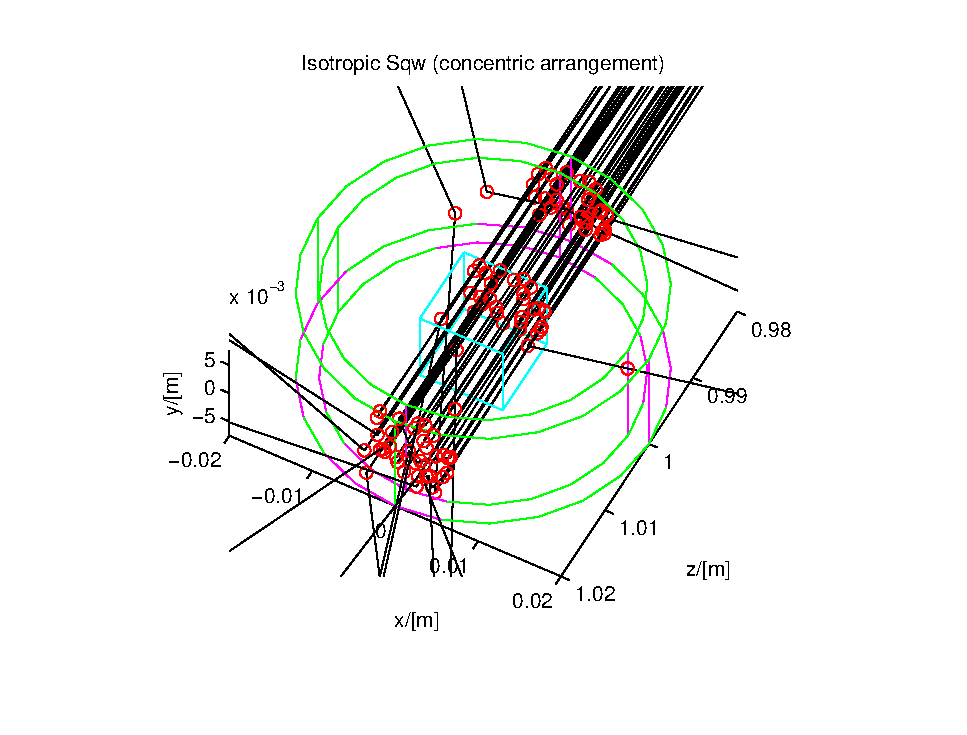
\includegraphics[width=\textwidth]{figures/sqw.eps}
     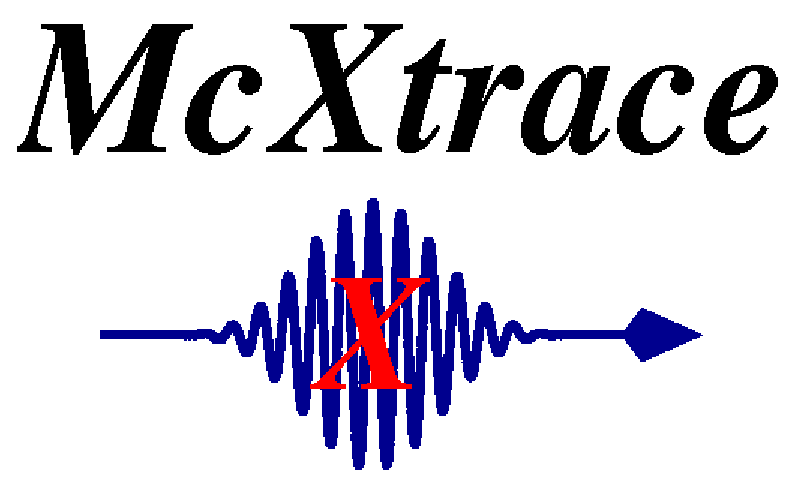
\includegraphics[width=8cm]{figures/mcxtrace-logo.eps}
   \end{center}
   \par \vfill \baselineskip 12dd
 \frtnbf\noindent Ris{\o} DTU, Roskilde, Denmark \par
 \vskip 4dd \noindent\ifcase\month\or
 January\or February\or March\or April\or May\or June\or
 July\or August\or September\or October\or November\or December\fi
 \space\number\year }

\let\reportlan=\relax
\def\month{3}                   % Released in November 2005
% Need to match front page line breaking.
\title{Component~Manual~for~\rlap{the}\\ % Avoid overfull message.
 X-ray-Tracing~Package\\
 \MCX, Version \version\ }
\author{Erik Bergb\"{a}ck Knudsen, Andrea Prodi, Peter Kj\ae r Willendrup and \\Kim Lefmann}
\maketitle
\endgroup

%\begin{center}
%  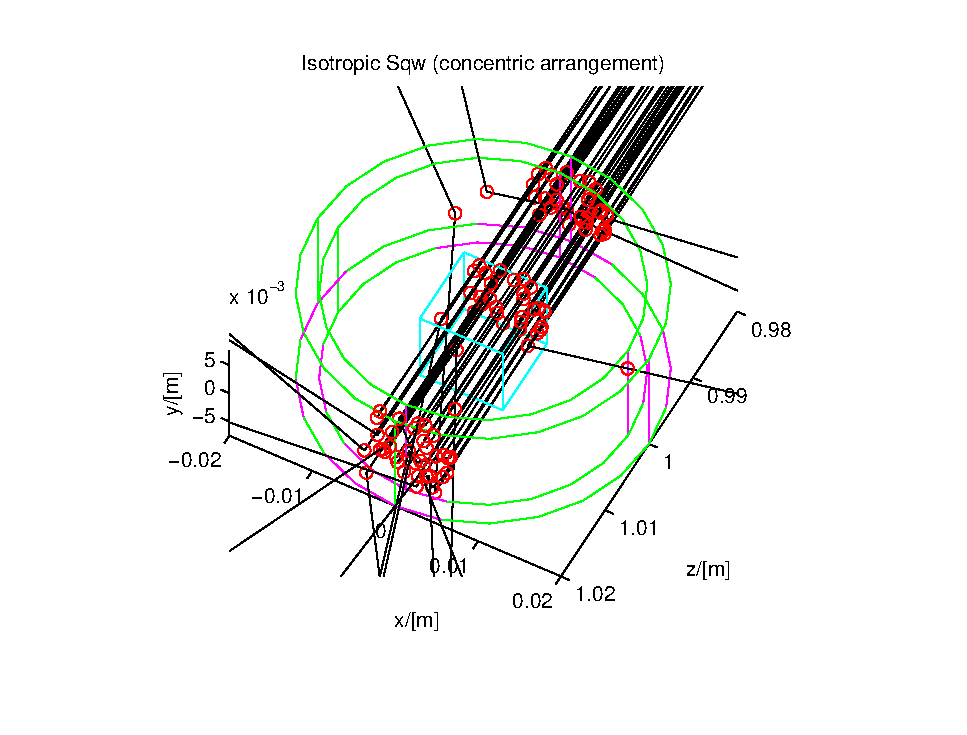
\includegraphics[width=4.5in]{figures/sqw.eps}
%\end{center}
%
% NOTE: Find a way to include this nice graphics on front page
% Currently this does not work?!?

\thispagestyle{empty}
% Emacs settings: -*-mode: latex; TeX-master: "manual.tex"; -*-

\begin{abstract}
The software package McStas is a tool for carrying out Monte Carlo
ray-tracing simulations of neutron scattering instruments with high
complexity and precision. The simulations can compute all aspects of the
performance of instruments and can thus be used to optimize the use of
existing equipment, design new instrumentation, and carry out virtual
experiments for e.g. training, experimental planning or data analysis. McStas
is based on a unique design where an automatic compilation process
translates high-level textual instrument descriptions into efficient
ANSI-C code. This design makes it simple to set up typical simulations
and also gives essentially unlimited freedom to handle more unusual
cases.

This report constitutes the reference manual for McStas, and,
together with the manual for the McStas components, it
contains documentation of most aspects of the program. It covers
the various ways to compile and run simulations, a description of the
meta-language used to define simulations, 
%a full description of all
%algorithms used to calculate the effects of the various optical
%components in instruments, 
and some example simulations performed with
the program.

\end{abstract}

\vskip\baselineskip\noindent
This report documents \MCS version \version, released \reldate
\vskip\baselineskip\noindent
The authors are:
\begin{quote}
\label{p:authors}
Peter Kj\ae r Willendrup \verb+<pkwi@fysik.dtu.dk>+ \\
Physics Department, Technical University of Denmark, Kongens Lyngby, Denmark 

Emmanuel Farhi \verb+<farhi@ill.fr>+ \\
Institut Laue-Langevin, Grenoble, France 

Erik Knudsen \verb+<erkn@fysik.dtu.dk>+ \\
Physics Department, Technical University of Denmark, Kongens Lyngby, Denmark 

Kim Lefmann \verb+<lefmann@nbi.dk>+ \\
Niels Bohr Institute, University of Copenhagen, Denmark

\end{quote}
as well as authors who left the project:
\begin{quote}
Peter Christiansen \verb+<pchristi@hep.lu.se>+\\
Materials Research Department, Ris{\o} National Laboratory, Roskilde, Denmark\\
Present address: University of Lund, Lund, Sweden\\
Klaus Lieutenant \verb+<klaus.lieutenant@helmholtz-berlin.de>+ \\
Institut Laue-Langevin, Grenoble, France \\
Present address: Helmotlz Zentrum Berlin, Germany \\
Kristian Nielsen \verb+<kristian-nielsen@mail.tele.dk>+ \\
Materials Research Department, Ris{\o} National Laboratory, Roskilde, Denmark\\
Presently associated with: MySQL AB, Sweden
\end{quote}
%Front page illustration:\\[\baselineskip]
%Simulated scattering from a vanadium sample
%taking into account the secondary extinction. See
%section~\ref{s:vanadium-result}.
\vfill
\noindent ISBN 978--87--550--3680--2
\par\noindent ISSN 0106--2840
\par\noindent\hbox{}\hfill
    Information Service Department $\cdot$ Ris{\o} DTU $\cdot$ \number\year
%    Information Service Department $\cdot$ Ris{\o} $\cdot$ \number\year
\par
\thispagestyle{empty}\clearpage





\tableofcontents
%\pagebreak
%\listoffigures
%\pagebreak
%\listoftables

% Emacs settings: -*-mode: latex; TeX-master: "manual.tex"; -*-

\addcontentsline{toc}{chapter}{\protect\numberline{}{Preface and acknowledgements}}
\chapter*{Preface and acknowledgements}
This document contains information on the x-ray scattering components
which are the building blocks for defining instruments
in the Monte Carlo Xray-tracing program \MCX version \version . The initial
release in June 2011 of version 1.0 was presented in Ref.~\cite{nn_10_20}.
The reader of this
document is not supposed to have specific knowledge of xray scattering,
but some basic understanding of physics is helpful in
understanding the theoretical background for the component functionality.
For details about setting up and running simulations, we refer to
the \MCX system manual \cite{mcxtracemanual}.
We assume familiarity with the use of
the C programming language.

%We especially like to thank Kristian Nielsen for laying a solid foundation
%for the \MCX\ system, which the authors of this manual benefit from daily.
We would like to explicitly thank all the partners in this project:
\begin{itemize}
\item The European Synchrotron Radiation Facility (ESRF), Grenoble, France
\item SAXSLAB Aps., Lundtofte, Denmark
\item Risø DTU, Roskilde, Denmark
\item \NBIlong
\item \Lifelong
\end{itemize}

As
\MCX has inherited much of its functionality from its sister \MCS we take the oppurtunity to thank 
Dir.~Kurt N.~Clausen, PSI, for his continuous
support to \MCS\ and for having initiated the project.
Continuous support to \MCS\ has also come from Prof.~Robert McGreevy, ISIS.

We have further benefited
from discussions with many other people in the scattering
community, too numerous to mention here.

The users who contributed components to this manual are acknowledged
as authors of the individual components. We encourage other
users to contribute components with manual entries for inclusion in
future versions of \MCX.

In case of errors, questions, or suggestions,
do not hesitate to
contact the user/developer community by writing to the user mailiing list \verb+mcxtrace-users@mcxtrace.órg+
or consult the \MCX\ home page~\cite{mcxtrace_webpage}. A special developement
website (shared with the sister project \MCS) complete with bug/request
reporting service is available \cite{trac_webpage}.

We would like to kindly thank all \MCX\ component contributors. This is the way we improve the software alltogether.

If you {\bfseries appreciate} this software, please subscribe to the \verb+mcxtrace-users@mcxtrace.org+ email list, send us a smiley message, and contribute to the package.

We also encourage you to refer to this software when publishing results, with the following citation:
\begin{itemize}
\item{E. B. Knudsen, et.al, J. Applied Cryst. {\bfseries 46}, pp 679, 2013.}
\end{itemize}







% Emacs settings: -*-mode: latex; TeX-master: "manual.tex"; -*-

\chapter{About the component library}
This \MCS Component Manual consists of the following major parts:\label{c:components}
\begin{itemize}
\item An introduction to the use of Monte Carlo methods in \MCS .
\item A thorough description of system components,
with one chapter per major category: Sources, optics,
monochromators, samples, monitors, and other components.
\item The \MCS library functions and definitions
  that aid in the writing of simulations and components in
  Appendix~\ref{c:kernelcalls}.
%\item A detailed explanation of the use of random numbers
%   in Appendix~\ref{s:random}.
\item An explanation of the \MCS terminology in Appendix~\ref{s:terminology}.
\end{itemize}
Additionally, you may refer to the list of example instruments
from the library in the \MCS User Manual.

\section{Authorship}
The component library is
maintained by the \MCS system group. A number of basic components
``belongs'' the \MCS system, and are supported and tested by the \MCS
team.

Other components are contributed
by specific authors, who are listed in the code for each component
they contribute as well as in this manual.
\MCS users are encouraged to send their
contributions to us for inclusion in future releases.

Some contributed components have later been taken over
for further development by the \MCS system
group, with permission from the original authors.
The original authors will still appear both in the component code and in the
\MCS manual.

\section{Symbols for neutron scattering and simulation}
In the description of the theory behind the component functionality
we will use the usual symbols {\bf r} for the position
$(x,y,z)$ of the particle (unit m), and {\bf v} for
the particle velocity $(v_x, v_y, v_z)$ (unit m/s).
Another essential quantity is the neutron wave vector
${\bf k} = m_{\rm n} {\bf v}/\hbar$ , where
$m_{\rm n}$ is the neutron mass. {\bf k} is usually given in
\AA$^{-1}$, while neutron energies are given in meV.
The neutron wavelength is the reciprocal wave vector,
$\lambda=2 \pi / k$.
In general, vectors are denoted by boldface symbols.

Subscripts "i" and "f" denotes ``initial'' and ``final'', respectively,
and are used in connection with the neutron state before and after
an interaction with the component in question.
%This is of particular importance in sample components, where the
%wave vector change is denoted the {\em scattering vector}
%\begin{equation}\label{eq:q-transfert}
%{\bf q} \equiv {\bf k}_{\rm i} - {\bf k}_{\rm f} .
%\end{equation}
%In analogy, the {\em energy transfer} is given by
%\begin{equation}\label{eq:w-transfert}
%\hbar \omega \equiv E_{\rm i}-E_{\rm f} =
%\frac{\hbar^2}{2 m_{\rm n}} \left( k_{\rm i}^2 - k_{\rm f}^2 \right).
%\end{equation}

The spin of the neutron is given a special treatment. Despite
the fact that each physical neutron has a well defined spin value,
the \MCS spin vector
{\bf s} can have any length between zero (unpolarized beam) and unity
(totally polarized beam). Further, all three cartesian components of
the spin vector are present simultaneously, although this is physically
not permitted by quantum mechanics.
For further details about polarization handling, you may refer to the Appendix~\ref{c:polarization}.

\section{Component coordinate system}
All mentioning of component geometry refer to
the local coordinate system of the individual component.
The axis convention is so that the $z$ axis is along
the neutron propagation axis, the $y$ axis is vertical up,
and the $x$ axis points left when looking along the $z$-axis,
completing a right-handed coordinate system.
Most components 'position' (as specified in the instrument description
with the \verb+AT+ keyword) corresponds to their input side at the nominal
beam position.
However, a few components are radial and thus positioned in their centre.
\index{Symbols}\index{Coordinates system}

Components are usually not designed to overlap.
This may lead to loss of neutron rays.
Warnings will be issued during simulation if sections of the instrument
are not reached by any neutron rays, or if neutrons are removed.
This is usually the sign of either overlapping components
or a very low intensity.\index{Removed neutron events}

\section{About data files}\index{Data files}\index{Library!read\_table-lib (Read\_Table)}
Some components require external data files,
e.g. lattice crystallographic definitions for Laue and powder pattern diffraction,
$S(q,\omega)$ tables for inelastic scattering,
neutron events files for virtual sources,
transmission and reflectivity files, etc.

Such files distributed with \MCS are located in the
\verb+data+ sub-directory of the McStas library.
Components that make use of the \MCS file system,
including the \verb+read-table+ library (see section \ref{s:read-table})
may access all \MCS data files without making local copies.
Of course, you are welcome to define your own data files,
and eventually contribute to \MCS if you find them useful.

File extensions are not compulsory but help in identifying relevant files per application. We list powder and liquid data files from the \MCS library in Tables \ref{t:powders-data} and \ref{t:liquids-data}. These files contain an extensive header describing physical properties with references, and are specially suited for the PowderN (see \ref{powder}) and Isotropic\_Sqw components (see \ref{s:isotropic-sqw}).

\begin{table}
  \begin{center}
    {\let\my=\\
    \begin{tabular}{|p{0.24\textwidth}|p{0.7\textwidth}|}
      \hline
       {\bf MCSTAS/data} & Description \\
       \hline
 *.lau & Laue pattern file, as issued from Crystallographica.
       For use with Single\_crystal, PowderN, and Isotropic\_Sqw.
       Data: [ h   k   l Mult. d-space 2Theta   F-squared ] \\
 *.laz & Powder pattern file, as obtained from Lazy/ICSD.
       For use with PowderN, Isotropic\_Sqw and possibly Single\_crystal.\\
 *.trm & transmission file, typically for monochromator crystals and filters.
       Data: [ k (Angs-1) , Transmission (0-1) ] \\
 *.rfl & reflectivity file, typically for mirrors and monochromator crystals.
       Data: [ k (Angs-1) , Reflectivity (0-1) ] \\
 *.sqw & $S(q,\omega)$ files for Isotropic\_Sqw component.
       Data: [q] [$\omega$] [$S(q,\omega)$]\\
      \hline
    \end{tabular}
    \caption{Data files of the \MCS library.}
    \label{t:comp-data}
    \index{Library!Components!data}
    }
  \end{center}
\end{table}

\begin{table}
  \begin{center}
    {\let\my=\\
    \begin{small}
    \begin{tabular}{|l|rrr|rr|p{0.2\textwidth}|}

      \hline
      {\bf MCSTAS/data} & $\sigma_{coh}$&$\sigma_{inc}$&$\sigma_{abs}$&$T_m$       & $c$    & Note \\
          File name     & [barns]     & [barns]    & [barns]    & [K]        & [m/s] & \\
      \hline
Ag.laz             & 4.407     & 0.58     &{\bf 63.3}      &1234.9    &2600&\\
Al2O3\_sapphire.laz & 15.683    & 0.0188   &0.4625    &2273      &   &\\
Al.laz             & 1.495     & 0.0082   &0.231     &933.5     &5100& .lau\\
Au.laz             & 7.32      & 0.43     &{\bf 98.65}     &1337.4    &{\bf 1740}&\\
B4C.laz            & 19.71     & 6.801    &{\bf 3068}      &2718      &     &\\
Ba.laz             & 3.23      & 0.15     &29.0      &1000      &{\bf 1620}&\\
Be.laz             & 7.63      & 0.0018   &0.0076    &1560      &13000&\\
BeO.laz            & 11.85     & 0.003    &0.008     &2650      &   & .lau\\
Bi.laz             & 9.148     & 0.0084   &0.0338    &544.5     &{\bf 1790}&\\
C60.lau            & 5.551     & 0.001    &0.0035    &          &   &\\
C\_diamond.laz      & 5.551     & 0.001    &0.0035    &4400      &18350 & .lau\\
C\_graphite.laz     & 5.551     & 0.001    &0.0035    &3800      &18350 & .lau\\
Cd.laz             & 3.04      & 3.46     &{\bf 2520}      &594.2     &2310&\\
Cr.laz             & 1.660     & 1.83     &3.05      &2180      &5940&\\
Cs.laz             & 3.69      & 0.21     &29.0      &301.6     &{\bf 1090}  & $c$ in liquid\\
Cu.laz             & 7.485     & 0.55     &3.78      &1357.8    &3570&\\
Fe.laz             & 11.22     & 0.4      &2.56      &1811      &4910&\\
Ga.laz             & 6.675     & 0.16     &2.75      &302.91    &2740&\\
Gd.laz             & 29.3      & 151      &{\bf 49700}     &1585      &2680&\\
Ge.laz             & 8.42      & 0.18     &2.2       &1211.4    &5400  & \\
H2O\_ice\_1h.laz     & 7.75      & 160.52   &0.6652    &273       &     &\\
Hg.laz             & 20.24     & 6.6      &{\bf 372.3}     &234.32    &{\bf 1407}&\\
I2.laz             & 7.0       & 0.62     &12.3      &386.85    &   &\\
In.laz             & 2.08      & 0.54     &{\bf 193.8}     &429.75    &{\bf 1215}&\\
K.laz              & .69       & 0.27     &2.1       &336.53    &{\bf 2000}&\\
LiF.laz            & 4.46      & 0.921    &{\bf 70.51}     &1140      &   &\\
Li.laz             & 0.454     & 0.92     &{\bf 70.5}      &453.69    &6000&\\
Nb.laz             & 8.57      & 0.0024   &1.15      &2750      &3480&\\
Ni.laz             & 13.3      & 5.2      &4.49      &1728      &4970&\\
Pb.laz             & 11.115    & 0.003    &0.171     &600.61    &{\bf 1260}&\\
Pd.laz             & 4.39      & 0.093    &6.9       &1828.05   &3070&\\
Pt.laz             & 11.58     & 0.13     &10.3      &2041.4    &2680&\\
Rb.laz             & 6.32      & 0.5      &0.38      &312.46    &{\bf 1300}  & \\
Se\_alpha.laz       & 7.98      & 0.32     &11.7      &494       &3350&\\
Se\_beta.laz        & 7.98      & 0.32     &11.7      &494       &3350&\\
Si.laz             & 2.163     & 0.004    &0.171     &1687      &2200&\\
SiO2\_quartza.laz   & 10.625    & 0.0056   &0.1714    &846       &      & .lau\\
SiO2\_quartzb.laz   & 10.625    & 0.0056   &0.1714    &1140      &      & .lau\\
Sn\_alpha.laz       & 4.871     & 0.022    &0.626     &505.08    &     &\\
Sn\_beta.laz        & 4.871     & 0.022    &0.626     &505.08    &2500&\\
Ti.laz             & 1.485     & 2.87     &6.09      &1941      &4140&\\
Tl.laz             & 9.678     & 0.21     &3.43      &577       &{\bf 818}&\\
V.laz              & .0184     & 4.935    &5.08      &2183      &4560&\\
Zn.laz             & 4.054     & 0.077    &1.11      &692.68    &3700&\\
Zr.laz             & 6.44      & 0.02     &0.185     &2128      &3800&\\
      \hline
    \end{tabular}\end{small}
    \caption{Powders of the \MCS library \cite{icsd_ill,ILLblue}. Low $c$ and high $\sigma_{abs}$ materials are highlighted. Files are given in LAZY format, but may exist as well in Crystallographica {\it .lau} format as well.}
    \label{t:powders-data}
    \index{Library!Components!data}
    }
  \end{center}
\end{table}

\begin{table}
  \begin{center}
    {\let\my=\\
    \begin{small}
    \begin{tabular}{|l|rrr|rr|p{0.2\textwidth}|}

      \hline
      {\bf MCSTAS/data} & $\sigma_{coh}$&$\sigma_{inc}$&$\sigma_{abs}$&$T_m$       & $c$    & Note \\
          File name     & [barns]     & [barns]    & [barns]    & [K]        & [m/s] & \\
      \hline
Cs\_liq\_tot.sqw                      & 3.69      & 0.21     &29.0      &301.6     &{\bf 1090}  & Measured \\
Ge\_liq\_coh.sqw and Ge\_liq\_inc.sqw & 8.42      & 0.18     &2.2       &1211.4    &5400  & Ab-initio MD \\
He4\_liq\_coh.sqw                     & 1.34      & 0        &0.00747   &0         &{\bf 240}   & Measured\\
Ne\_liq\_tot.sqw                      & 2.62      & 0.008    &0.039     &24.56     &{\bf 591}   & Measured\\
Rb\_liq\_coh.sqw and Rb\_liq\_inc.sqw & 6.32      & 0.5      &0.38      &312.46    &{\bf 1300}  & Classical MD \\
Rb\_liq\_tot.sqw                      & 6.32      & 0.5      &0.38      &312.46    &{\bf 1300}  & Measured \\
      \hline
    \end{tabular}\end{small}
    \caption{Liquids of the \MCS library \cite{icsd_ill,ILLblue}. Low $c$ and high $\sigma_{abs}$ materials are highlighted.}
    \label{t:liquids-data}
    \index{Library!Components!data}
    }
  \end{center}
\end{table}

\MCS itself generates both simulation and monitor data files, which structure is explained in the User Manual (see end of chapter 'Running \MCS ').

\section{Component source code}
Source code for all components may be found in the \verb+MCSTAS+ library
subdirectory of the McStas installation;
the default is \verb+/usr/local/lib/mcstas/+
on Unix-like systems and \verb+C:\mcstas\lib+ on Windows systems, but it may be
changed using the \verb+MCSTAS+ environment variable.
\index{Environment variable!MCSTAS}

In case users only require to add new features, preserving the existing features of a component,
using the \verb+EXTEND+ keyword\index{Keyword!EXTEND} in the instrument description file is recommended. For larger modification of a component, it is advised to make a copy
of the component file into the working directory.
A component file in the local directory will in \MCS take precedence over
a library component of the same name.

\section{Documentation}
As a complement to this Component Manual, we encourage users to use
the \verb+mcdoc+ front-end which enables to display both the
catalog of the \MCS library, e.g using: \index{Tools!mcdoc}
\begin{lstlisting}
  \verb|mcdoc|
\end{lstlisting}
as well as the documentation of specific components, e.g with:
\begin{lstlisting}
  \verb|mcdoc --text| {\it name} \\
  \verb|mcdoc| {\it file.comp}
\end{lstlisting}
The first line will search for all components matching the {\it name},
and display their help section as text. For instance, \verb+mcdoc .laz+ will list all available Lazy data files, whereas \verb+mcdoc --text Monitor+ will list most Monitors.
The second example will display the help corresponding to
the {\it file.comp} component, using your
BROWSER\index{Environment variable!BROWSER} setting, or as text if unset.
The \verb+--help+ option will display the command help, as usual.

An overview of the component library is also given at the \MCS home page \cite{mcstas_webpage} and in the User Manual \cite{mcstasmanual}.

\section{Component validation}

Some components were checked for release 1.9: the Fermi choppers, the velocity selectors, 2 of the guide components and Source\_gen. The results are sumarized in a talk available online (\verb+http://www.ill.fr/tas/mcstas/doc/ValMcStas.pdf+).

Velocity selector and Fermi chopper were treated as black boxes and the resulting line shapes cross-checked against analytical functions for some cases.
The component 'Selector' showed no dependence on the distance between guide and selector axe. This is corrected at the moment. Apart from that the component yielded correct results.
That was different with the Fermi chopper components. The component 'Chopper\_Fermi', which has been part of the \MCS distribution for a long time, gave wrong results and was removed from the package. The new 'Vitess\_ChopperFermi' (transferred from the VITESS package) showed mainly correct behaviour. Little bugs were corrected after the first tests. At the moment, there is only the problem left that it underestimates the influence of a shadowing cylinder. With the contributed 'FermiChopper' component, there were also minor problems, which are all corrected in the meantime.

For the guides, several trajectories through different kinds of guides (straight, convergent, divergent) were calculated analytically and positions, directions and losses of reflections compared to the values calculated in the components. This was done for 'Guide' and 'Guide\_gravity'; in the latter case calculations were performed with and without gravity. Additionally a cross-check against the VITESS guide module was performed. Waviness, chamfers and channels were not checked.
After correction of a bug in 'Guide\_gravity', both components worked perfectly (within the conditions tested).

'Source\_gen' was cross-checked against the VITESS source module for the case of 3 Maxwellians describing the moderator characteristic and typical sizes the guide and its distance to the moderator. It showed the same line shape as a functions of wavelength and divergence and the same absolute values.

\section{Disclaimer, bugs}\index{Bugs}

We would like to emphasize that the usage of both the \MCS software, as well as its components are the responsability of the users. Indeed, obtaining accurate and reliable results requires a substantial work when writing instrument descriptions. This also means that users should read carefully both the documentation from the manuals \cite{mcstasmanual} and from the component itself (using \verb+mcdoc+ {\it comp}) before reporting errors. Most anomalous results often originate from a wrong usage of some part of the package.

Anyway, if you find that either the documentation is not clear, or the behavior of the simulation is undoubtedly anomalous, you should report this to us at \verb+mcstas@risoe.dk+ and refer to our special bug/request reporting service \cite{mczilla_webpage}.

\chapter{Monte Carlo Techniques and simulation strategy}
\label{s:MCtechniques}\index{Monte Carlo method}

This chapter explains the simulation strategy and the Monte Carlo
techniques used in \MCS. We first explain the concept of the neutron
weight factor, and discuss the statistical errors in dealing with sums
of neutron weights.  Secondly, we give an expression for how the weight
factor transforms under a Monte Carlo choice and specialize this
to the concept of direction focusing.  Finally, we present a way of
generating random numbers with arbitrary distributions.
More details are available in the Appendix concerning random numbers.


%%%%%%%%%%%%%%%%%%%%%%%%%%%%%%%%%%%%%%%%%%%%%%%%%%%%%%%%%%%%%%%%%%%%%%%%%%%%%%%%
\section{Neutron spectrometer simulations}

%-------------------------------------------------------------------------------
\subsection{Monte Carlo ray tracing simulations}
The behavior of a neutron scattering instrument can in principle be described by a complex integral over all relevant parameters, like initial neutron energy and divergence, scattering vector and position in the sample, etc. However, in most relevant cases, these integrals are not solvable analytically, and we hence turn to Monte Carlo methods. The neutron ray-tracing Monte Carlo method has been used widely for guide studies \cite{Copley93,Farhi02,Schanzer04}, instrument optimization and design \cite{Zsigmond04,Lieutenant05}. Most of the time, the conclusions and general behavior of such studies may be obtained using the classical analytic approaches, but accurate estimates for the flux, resolution and generally the optimum parameter set, benefit considerably from MC methods.

Mathematically, the Monte-Carlo method is an application of the law of large numbers \cite{James80,Grimmett92}. Let $f(u)$ be a finite continuous integrable function of parameter $u$ for which an integral estimate is desirable. The discrete statistical mean value of $f$ (computed as a series) in the uniformly sampled interval $a < u < b$ converges to the mathematical mean value of $f$ over the same interval.

\begin{equation}
\lim_{n \rightarrow \infty} \frac{1}{n} \sum_{i=1, a \leq u_i \leq b}^n f(u_i) = \frac{1}{b-a}\int_a^b f(u) du
\end{equation}

In the case were the $u_i$ values are regularly sampled, we come to the well known midpoint integration rule. In the case were the $u_i$ values are randomly (but uniformly) sampled, this is the Monte-Carlo integration technique. As random generators are not perfect, we rather talk about \emph{quasi}-Monte-Carlo technique. We encourage the reader to consult James \cite{James80} for a detailed review on the Monte-Carlo method.

%%%%%%%%%%%%%%%%%%%%%%%%%%%%%%%%%%%%%%%%%%%%%%%%%%%%%%%%%%%%%%%%%%%%%%%%%%%%%%%%
\section{The neutron weight}
\label{s:probweight}
\index{Weight|textbf}
\index{Neutron!weight|textbf}

A totally realistic semi-classical simulation will require that
each neutron is at any time either present or lost.
In many instruments, only a very
small fraction of the initial neutrons will ever be detected, and
simulations of this kind will therefore waste much time in dealing
with neutrons that never hit the relevant detector or monitor.

An important way of speeding up calculations is to introduce
a neutron "weight factor" for each simulated neutron ray and to
adjust this weight according to the path of the ray.
If {\em e.g.}\ the reflectivity of a certain
optical component is 10\%, and only reflected neutrons ray are
considered later in the simulations, the neutron
weight will be multiplied by 0.10 when passing this component,
but every neutron is allowed to reflect in the component.
In contrast, the totally realistic simulation of the component
would require in average ten incoming neutrons for each reflected one.

Let the initial neutron weight be $p_0$ and let us denote the weight
multiplication factor in the $j$'th component by $\pi_j$.  The resulting
weight factor for the neutron ray after passage of the $n$ components in the instrument
becomes the product of all contributions
\begin{equation}
\label{e:probprod}
p = p_n = p_0 \prod_{j=1}^n \pi_j .
\end{equation}
Each adjustment factor should be $0 < \pi_j < 1$, except in special
circumstances, so that total flux can only decrease through the
simulation, see section \ref{s:weighttransform}. For convenience, the value of $p$ is updated (within each component)
during the simulation.

Simulation by weight adjustment is performed
whenever possible. This includes
\begin{itemize}
\item Transmission through filters and windows.
\item Transmission through Soller blade collimators and velocity
  selectors
 (in the approximation
 which does not take each blade into account).
\item Reflection from monochromator (and analyzer) crystals
 with finite reflectivity and mosaicity.
\item Reflection from guide walls.
\item Passage of a continuous beam through a chopper.
\item Scattering from all types of samples.
\end{itemize}

%-------------------------------------------------------------------------------
\subsection{Statistical errors of non-integer counts}
\label{s:staterror}
\index{Variance}
\index{Error estimate}
\index{Statistics!uncertainty}
\index{Neutron!statistical uncertainty}

In a typical simulation, the result will consist of a
count of neutrons histories ("rays") with different weights. The
sum of these weights is an estimate of the mean number of neutrons
hitting the monitor (or detector) per second in a ``real'' experiment.
One may write the counting result as
\begin{equation}
\label{psum}
I = \sum_i p_i = N \overline{p} ,
\end{equation}
where $N$ is the number of rays hitting the detector and the horizontal bar
denotes averaging.
By performing the weight transformations, the (statistical)
mean value of $I$ is unchanged. However, $N$ will in general be enhanced,
and this will improve the accuracy of the simulation.

To give an estimate of the statistical error, we proceed as follows:
Let us first for simplicity assume that all the counted neutron weights are
almost equal, $p_i \approx \overline{p}$,
and that we observe a large number of neutrons, $N \geq 10$.
Then $N$ almost follows a normal distribution
with the uncertainty $\sigma(N) = \sqrt{N}$
\footnote{This is not correct in a
situation where the detector counts a large fraction of the
neutron rays in the simulation, but we will neglect that for now.}.
Hence, the statistical uncertainty of the observed intensity becomes
\begin{equation} \label{e:sigI1}
 \sigma(I) = \sqrt{N} \overline{p} = I / \sqrt{N} ,
\end{equation}
as is used in real neutron experiments (where $\overline{p} \equiv 1$).
For a better approximation we return to Eq.~(\ref{psum}).
Allowing variations in both $N$ and $\overline{p}$,
we calculate the variance of the resulting intensity,
assuming that the two variables are statistically independent:
\begin{equation}
\sigma^2(I) = \sigma^2(N) \overline{p}^2 + N^2 \sigma^2(\overline{p}) .
\end{equation}
Assuming as before that $N$ follows a normal distribution, we reach
$\sigma^2(N) \overline{p}^2 = N \overline{p}^2$.
Further, assuming that the individual weights, $p_i$,
follow a Gaussian distribution (which in some cases is far from the truth)
we have
$N^2 \sigma^2(\overline{p}) = \sigma^2(\sum_i p_i) = N \sigma^2(p_i)$
and reach
\begin{equation}
\sigma^2(I) = N \left( \overline{p}^2 + \sigma^2(p_i) \right).
\end{equation}
The statistical variance of the $p_i$'s is estimated by
$\sigma^2(p_i) \approx  (\sum_i p_i^2 - N \overline{p}^2) / (N-1)$.
The resulting variance then reads
\begin{equation}
\sigma^2(I) = \frac{N}{N-1} \left( \sum_i p_i^2 - \overline{p}^2  \right) .
\end{equation}
For almost any positive value of $N$, this is very well approximated
by the simple expression
\begin{equation}
\sigma^2(I) \approx \sum_i p_i^2 .
\end{equation}
As a consistency check, we note that for all $p_i$ equal, this reduces to
eq.~(\ref{e:sigI1})

In order to compute the intensities and uncertainties, the monitor/detector components
in \MCS will keep track of
$N=\sum_i p_i^0, I=\sum_i p_i^1$, and $M_2 = \sum_i p_i^2$.

%%%%%%%%%%%%%%%%%%%%%%%%%%%%%%%%%%%%%%%%%%%%%%%%%%%%%%%%%%%%%%%%%%%%%%%%%%%%%%%%
\section{Weight factor transformations during a Monte Carlo
 choice}
\label{s:weighttransform}
\index{Weight!transformation}
\index{Neutron!weight!transformation}

When a Monte Carlo choice must be performed, {\em e.g.} when the
initial energy and direction of the neutron ray is decided at the source,
it is important to adjust the neutron weight so that the combined
effect of neutron weight change and Monte Carlo probability
of making this particular choice
equals the actual physical properties we like to model.

Let us follow up on the simple example of transmission.
The probability of transmitting the real neutron is $P$, but we make
the Monte Carlo choice of transmitting the neutron ray each time:
$f_\mathrm{MC}=1$. This must be reflected on the choice of weight multiplier
$\pi_j=P$. Of course, one could simulate without weight factor
transformation, in our notation written as $f_\mathrm{MC}=P, \pi_j=1$. To
generalize, weight factor transformations are given by the master equation
%In the ``real'' semi-classical world, there is a distribution
%(probability density) for the neutrons in the six dimensional
%(energy, direction, position) space of
%$\Pi(E,\Ombold,\textbf{r}) = dP/(dE d\Ombold d^3\textbf{r})$ depending upon
%the source temperature, geometry {\em etc.}\ In the
%Monte Carlo simulations, the six coordinates are for efficiency reasons
%in general picked from another distribution:
%$f_\mathrm{MC}(E,\Ombold,\textbf{r}) \neq \Pi(E, \Ombold,\textbf{r})$,
%since one would {\em e.g.} often generate
%only neutrons within a certain parameter interval.
%However, we must then require that the weights are adjusted
%by a factor $\pi_j$ (in this case: $j=1$) so that
\begin{equation} \label{e:probrule}
f_\mathrm{MC} \pi_j = P .
\end{equation}
%For the sources present in version \version,
%only the $(\Ombold, \textbf{r})$ dependence of the correction factors
%are taken into account.

This probability rule is general, and holds also if, e.g., it is decided to
transmit only half of the rays $(f_\mathrm{MC}=0.5)$.
An important different example
is elastic scattering from a powder sample,
where the Monte-Carlo choices are the particular powder line to scatter from,
the scattering position within the sample and the final neutron direction
within the Debye-Scherrer cone. This weight transformation is much more complex than described above, but still boils down to obeying the master transformation rule \ref{e:probrule}.

%-------------------------------------------------------------------------------
\subsection{Direction focusing}
\index{Monte Carlo method!direction focusing}
\label{s:focus}
\index{Focusing!importance sampling}
\index{Direction focusing}
\index{Importance sampling!direction focusing}

An important application of weight transformation is direction focusing.
Assume that the sample scatters the neutron rays in many directions.
In general, only neutron rays in some of these directions will
stand any chance of being detected. These directions we call
the {\em interesting directions}.
The idea in focusing is to avoid wasting computation time on
neutrons scattered in the other directions.
This trick is an instance of what in Monte Carlo terminology
is known as {\em importance sampling}. % \cite{importance}.

If {\em e.g.} a sample scatters isotropically
over the whole $4\pi$ solid angle, and all interesting
directions are known to be contained within a certain
solid angle interval $\Delta \Ombold$, only these solid angles
are used for the Monte Carlo choice of scattering direction.
This implies $f_\mathrm{MC}(\Delta\Omega) = 1$. However, if the physical
events are distributed uniformly over the unit sphere, we would have
$P(\Delta\Omega) = \Delta\Omega / (4\pi)$, according to Eq.~(\ref{e:probrule}).
One thus ensures that the mean simulated intensity is unchanged
during a "correct" direction focusing, while a too narrow focusing will
result in a lower (\textit{i.e.} wrong) intensity, since
we cut neutrons rays that should have reached the final detector.

\begin{figure}[htb!]
\begin{center}
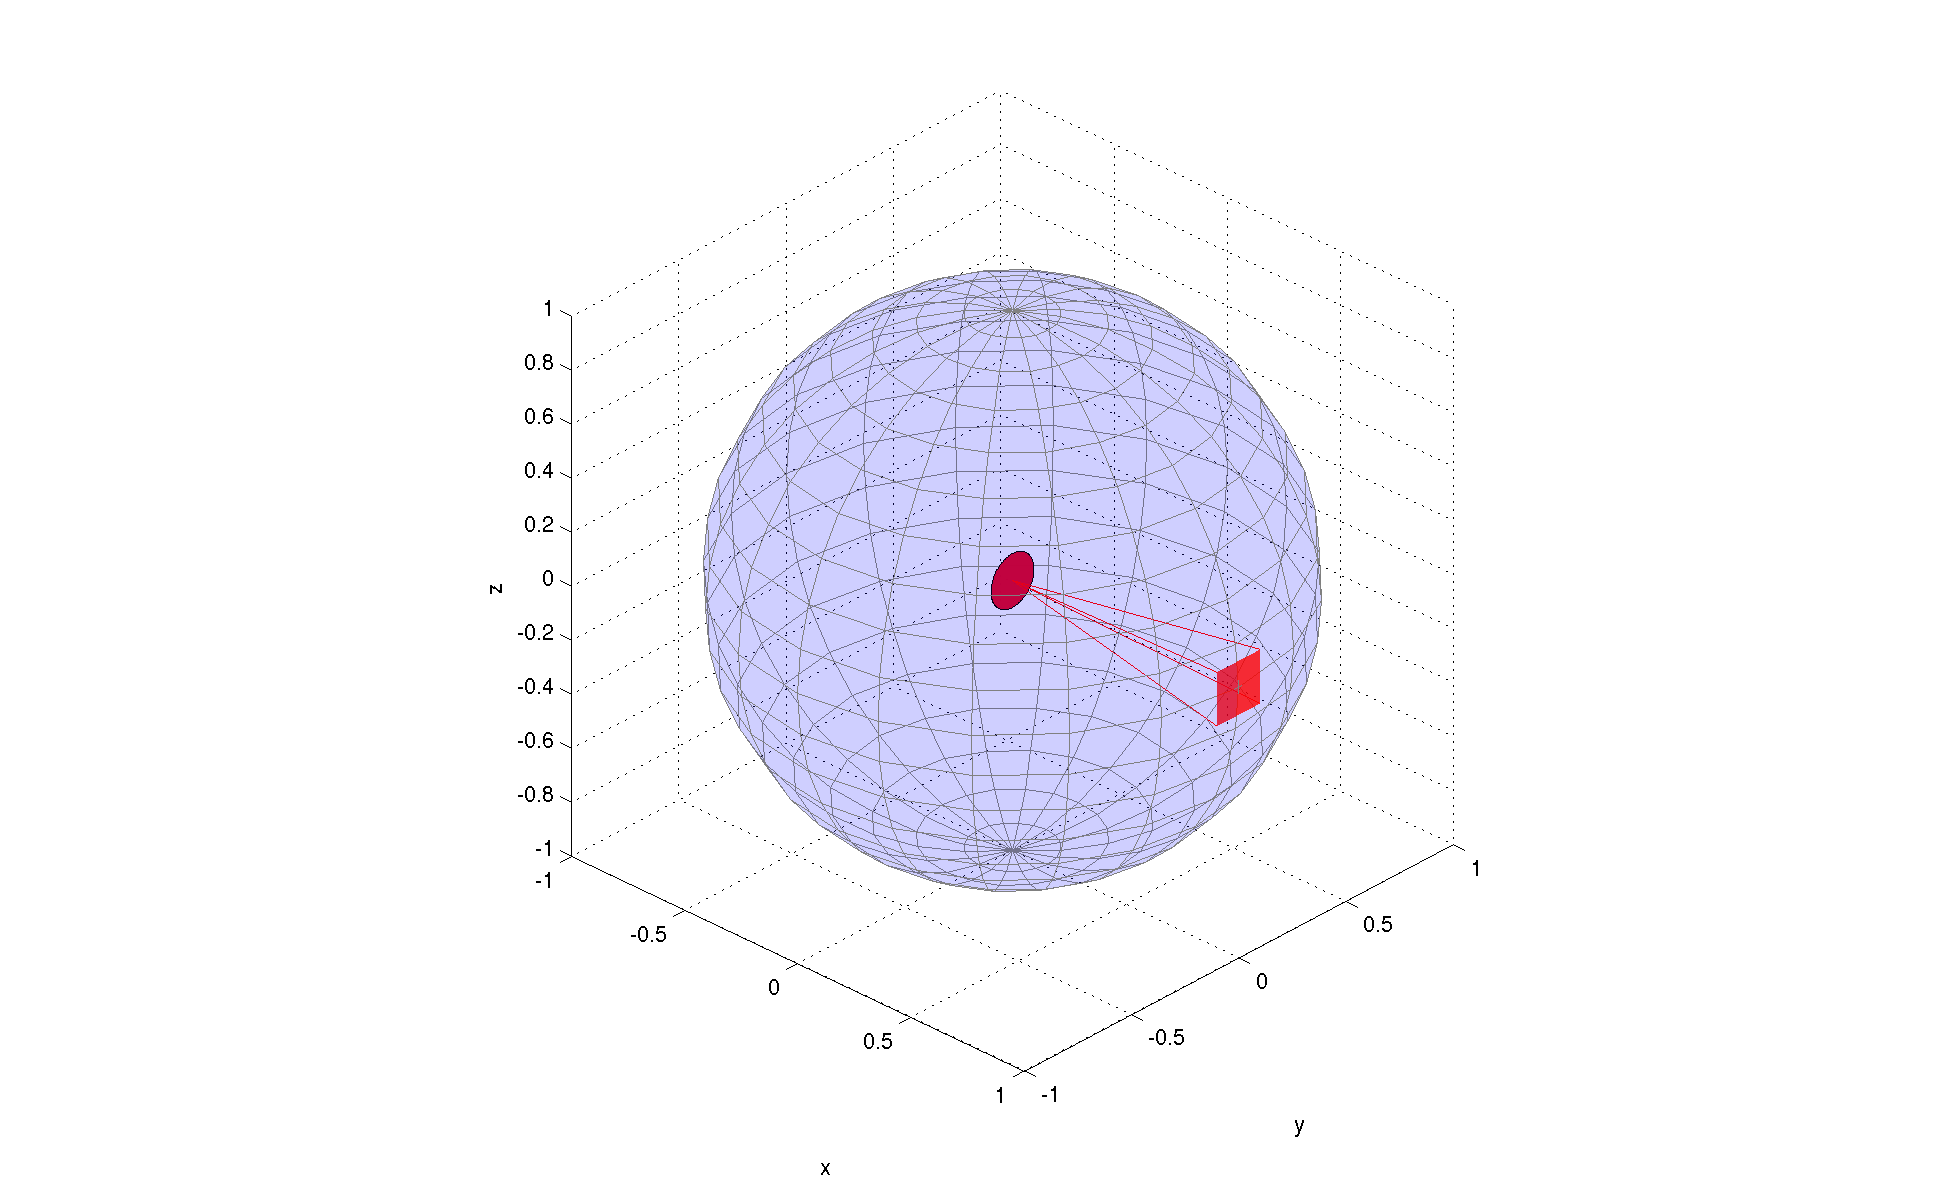
\includegraphics[width=.8\textwidth]{figures/focusing}
\end{center}
\caption{Illustration of the effect of direction focusing in \MCS
  . Weights of neutrons emitted into a certain solid angle are
  scaled down by the full unit sphere area.}
\label{fig:focusing}
\end{figure}

\section{Adaptive and Stratified sampling}
\index{Monte Carlo method!adaptive sampling}
\index{Monte Carlo method!stratified sampling}
\index{Adaptive sampling}
\index{Stratified sampling}
\index{Sampling}
\index{Variance reduction}

Another strategy to improve sampling in simulations
is \emph{adaptive importance sampling} (also called variance reduction technique), % \cite{importance},
where \MCS during the simulations will determine
the most interesting directions and gradually change
the focusing according to that.
Implementation of this idea is
found in the \textbf{Source\_adapt} and \textbf{Source\_Optimizer} components.
%, described in section~\ref{s:Source_adapt}.

An other class of efficiency improvement technique is the so-called \emph{stratified sampling}. It consists in partitioning the event distributions in representative sub-spaces, which are then all sampled individually. The advantage is that we are then sure that each sub-space is well represented in the final integrals. This means that instead of shooting $N$ events, we define $D$ partitions and shoot $r=N/D$ events in each partition. In conjunction with adaptive sampling, we may define partitions so that they represent 'interesting' distributions, e.g. from events scattered on a monochromator or a sample. The sum of partitions should equal the total space integrated by the Monte Carlo method, and each partition must be sampled randomly.

\index{Virtual sources}
In the case of \MCS, an ad-hoc implementation of adaptive stratified is used when repeating events, such as in the Virtual sources (Virtual\_input, Vitess\_input, Virtual\_mcnp\_input, Virtual\_tripoli4\_input) and when using the SPLIT keyword in the TRACE section on instrument descriptions. We emphasize here that the number of repetitions $r$ should not exceed the dimensionality of the Monte Carlo integration space (which is $d=10$ for neutron events) and the dimensionality of the partition spaces, i.e. the number of random generators following the stratified sampling location in the instrument.

\section{Accuracy of Monte Carlo simulations}
\index{Monte Carlo method!accuracy}

When running a Monte Carlo, the meaningful quantities are obtained by integrating random events into a single value (e.g. flux), or onto an histogram grid. The theory \cite{James80} shows that the accuracy of these estimates is a function of the space dimension $d$ and the number of events $N$. For large numbers $N$, the central limit theorem provides an estimate of the relative error as $1/\sqrt{N}$. However, the exact expression depends on the random distributions.

\MCS uses a space with $d=10$ parameters to describe neutrons (position, velocity, spin, time). We show in Table \ref{t:mc_accuracy} a rough estimate of the accuracy on integrals as a function of the number of records reaching the integration point. This stands both for integrated flux, as well as for histogram bins - for which the number of events per bin should be used for $N$.

\begin{table}
  \begin{center}
  {\let\my=\\
    \begin{tabular}{|c|c|}
    \hline
    Records       & Accuracy \\
    \hline
    $10^3$ & 10 \% \\
    $10^4$ & 2.5 \% \\
    $10^5$ & 1 \% \\
    $10^6$ & 0.25 \% \\
    $10^7$ & 0.05 \% \\
    \hline
    \end{tabular}
    \caption{Accuracy estimate as a function of the number of statistical events used to estimate an integral with \MCS.}
    \label{t:mc_accuracy}
  }
  \end{center}
\end{table}


% Emacs settings: -*-mode: latex; TeX-master: "manual.tex"; -*-

\chapter{Source components}
\label{c:sources}
\index{Sources|textbf}
\index{Library!Components!sources}

\MCX\ contains a number of different source components,
and any simulation will usually contain exactly one of these sources.
The main function of a source is to determine a set of initial
parameters $(\mathbf{r}, \mathbf{k}, t)$
for each photon ray. This is done by Monte Carlo choices from
suitable distributions. For example, in most present sources
the initial position is
found from a uniform distribution over the source surface.
The initial photon wavenumber
is selected within an interval of either the corresponding energy or the corresponding wavelength.

For pulsed sources, the choice of the emission time, $t$,
is being made on basis of detailed analytical expressions.
For other sources, $t$ is set to zero.
In the case one would like to use a steady state source
with time-of-flight settings,
the emission time of each photon ray should be determined using
a Monte Carlo choice. This may be achieved by
the \verb+EXTEND+ keyword in the instrument description source
as in the example below:\index{Keyword!EXTEND}

\begin{verbatim}
  TRACE

  COMPONENT MySource=Source_pt(...) AT (...)
  EXTEND
  %{
    t = 1e-3*randpm1(); /* set time to +/- 1 ms */
  %}
\end{verbatim}
Also take a look at the \textbf{Chopper\_simple} component.

\subsection{Photon flux and Brilliance}
\label{s:xray-flux}
The flux of the sources deserves special attention. The total
intensity is defined as the sum of weights of all emitted x-rays
during one simulation
(the unit of total photon weight is thus photons per second).
The flux, $\psi$, at an instrument is defined as intensity per area perpendicular
to the beam direction.

The source Brilliance, $\Phi$, is defined in different units (See e.g. \cite{als2011elements}):
the number of photon rays emitted per second from a
\SI{1}{\square mm} area on the source surface,
with direction within a 1~\si{\square m \radian} angle window,
and with wavelength within a 1\% interval.
The total intensity of real photons emitted towards a given diaphragm
(units: ph./s) is therefore (for constant $\Phi$):
\begin{equation}
I_\mathrm{total} = \Phi A \Delta\Omega \Delta\lambda ,
\end{equation}
where $A$ is the source area, $\Delta\Omega$ is the solid angle of the
diaphragm as seen from the source surface, and $\Delta\lambda$ is the
width of the wavelength interval in which photons are emitted (assuming
a uniform wavelength spectrum).

The simulations are performed so that detector intensities
are independent of the number of photon histories simulated
(although more photon histories will give better statistics).
If $N_\mathrm{sim}$ denotes the number of
x-ray histories to simulate, the initial photon weight $p_0$ must be set to
\begin{equation}
\label{proprule}
p_0 = \frac{N_\mathrm{total}}{N_\mathrm{sim}} =
    \frac{\Phi(\lambda)}{N_\mathrm{sim}} A \Omega \Delta\lambda ,
\end{equation}
where the source brilliance is now given a $\lambda$-dependence.

As a start, we recommend new \MCX\ users to use the
\textbf{Source\_flat} component.
For a slightly more realistic sources are supply \textbf{Source\_flat} with a spectrum file (for instance
generated by SPECTRA~\cite{spectra}) or \textbf{Source\_gaussian}.

Optimizers can dramatically improve the statistics, but may occasionally
give wrong results, due to misleaded optimization.
You should always check such simulations with (shorter) non-optimized ones.

Other ways to speed-up simulations are to read events from a file.
See section \ref{s:sources-seealso} for details.

\begin{figure}
  \begin{center}
    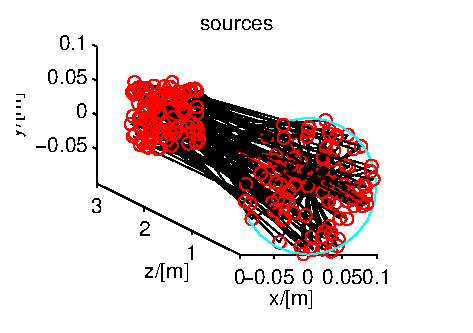
\includegraphics[width=0.75\textwidth]{figures/sources.eps}
  \end{center}
\caption{A circular source component (at z=0) emitting photon rays randomly, either from a model, or from a data file.}
\label{f:source}
\end{figure}

\newpage
\section{Source\_pt: A mathematical point emitting photons with a spectrum either uniform, gaussian or generated from a datafile}
\label{source-pt}
\index{Sources!Point source}
\mcdoccomp{sources/Source_pt.parms}

The simplest source model, where a mathematical point source at $(0,0,0)$ emits photons. The wavevector of the emitted photons
is picked randomly in a defining aperture $focus\_xw$ by $focus\_yh$ m at $(0,0,dist)$. 
Please note that this aperture is merely a
virtual aperture used to reduce the sampling space. This has a few
implications: Other components may be placed without reference to the aperture,
but if the aperture does not fill the full acceptance window of subsequent
components your simulations will be biased. The aperture is simply there to provide efficient sampling.

If a $spectrum\_file$ is not supplied, the xray
is given a weight which is the total wavelength-integrated intensity downscaled
by the
solid subtended by the definning aperture.

If a $spectrum\_file$ \emph{is} supplied, a slightly different strategy is adopted. In this case the
wavelength/energy range implied by the datafile is sampled unformly and each ray is assigned
a weight corresponding to the intensity indicated by linear interpolation between datapoints
at that wavelength. This implies an oversampling of weak parts of the intensity spectrum.

Currently only completely coherent or fully incoherent beams are supported. If
$phase$ is specified emitted photons be assigne dthat phase, otherwise it is
chosen randomly.


\section{Source\_flat: A flat surface emitting photons with a spectrum either uniform, gaussian or generated from a datafile}
\label{source-flat}
\index{Sources!Flat surface source}
\mcdoccomp{sources/Source_flat.parms}

A simple source model, with a flat surface emitting photons. The surface in the
$xy$-plane is specified as a rectangle with dimensions
$x_{width}\times y_{height}$ m, or as a circle w radius,$r$. 
The initial xray position is chosen randomly in the source surface --- its
wavevector is chosen randomly (exactly as in the case of \verb+Source\_pt+ (section \ref{source_pt}) in the defining aperture with height $h$ and
width $w$ placed at $(0,0,dist)$. 

Just as for \verb+Source\_pt+ the aperture is for efficiency purposes and, if misused, may cause biasing

A spectrum file may be supplied as for \verb+Source\_pt+.

Currently only fully coherent or incoherent beams are supported. If $phase$ is set (and not $randomphase$ which takes precedence) a phase is set such that a photon emitted from $(x,y,0)$ will be in phass with a photon at $(0,0,0)$, which has the phase $phase$..


\section{Source\_div: A continuous source with specified divergence}
\label{source-div}
\index{Sources!Continuous source with specified divergence}

%\component{Source\_div}{System}{ $w$, $h$, $\delta_h$, $\delta_v$, $E_0$, $\Delta E$}{$\lambda_0$, $\Delta\lambda$, gauss}{Validated. t=0}
\mcdoccomp{sources/Source_div.parms}

{\bf Source\_div} is a rectangular source, $w \times h$, which emits a
beam of a specified divergence around the direction of the $z$ axis.
The beam intensity is uniform over
the whole of the source, and the energy (or wavelength) distribution
of the beam is uniform over the specified energy range
$E_0 \pm \Delta E$ (in meV), or alternatively
the wavelength range $\lambda_0 \pm \delta\lambda$ (in \AA ).

The source divergences are $\delta_h$ and $\delta_v$ (FWHM in degrees).
If the \verb+gauss+ flag is set to 0 (default),
the divergence distribution is uniform, otherwise it is Gaussian.

This component may be used as a simple model of the
beam profile at the end of a guide or at the sample position.



\section{Source\_gaussian: the model has a gaussian distribution of intensity}
\label{source-gaussian}
\index{Sources!Source\_gaussian}
\mcdoccomp{sources/Source_gaussian.parms}

A simplified version of a completely incoherent source of horizontal and
vertical sizes \textit{sig\_x} and \textit{sig\_y} respectively with angular divergence
\textit{sigPr\_x} and \textit{sigPr\_y}. Can be used to model an undulator source emitting
a photon beam that has gaussian distribution.
This naturally generates a larger Gaussian profile at a distance. A sampling window at $(0,0,\mathit{dist})$
may be specified by the parameters \textit{focus\_xw} and \textit{focus\_yh}, which restricts the
sampling phases space of the emitted photons (See section~\ref{source\_pt} for details).

The energy spectrum emitted by \textbf{Source\_gaussian} source is completely analogous to \textbf{Source\_pt}, as is 
its photon phase functionality.


\section{Source\_lab: X-ray tube laboratory source}
\label{s:source-div}
\index{Sources!X-ray tube laboratory source}

\mcdoccomp{sources/Source_lab.parms}

\textbf{Source\_lab} is a model of a laboratory X-ray tube. An electron ray hits a
target of specified material. Currently, only single materiual targets are
allowed\footnote{To model multiple material targets one could construct a model with two
or more sources simultaneously. This has consequences for intensity of the source which should be downscaled accordingly.}.

An electron beam of transverse crossection ($x_0,z_0$) and energy $E_0$
impinges on the target of material. Wrt. the electron beam, the target is
considereded infinitely thick. The beam is considered to have uniform
intenisty. Thus, the spatial distribution of x-ray generation will be
exponential in the depth of the material.

Further, an exit aperture is defined with dimensions ($x_{width},y_{height}$). The centre of the aperture is situated at a distance $wd$ m from where the electron beam hits the target slab at an elevation of $take\_off$ (see Figure~\ref{f:source_lab}).  
Note that the center of the exit aperture is the reference point of the
\verb+Source\_lab+ coordinate system. In other words, the position specified in
the instrument file \verb+AT (x,y,z) RELATIVE somewhere+ is the center of the
exit aperture. Also note that the exit aperture is merely an opening. If the material absorption of the window, e.g. Be, is to be taken into account a \verb+Filter.comp+ (section~\ref{s:filter}) could be inserted after the exit aperture. 

\begin{figure}
\label{f:source_lab}
\caption{Geometry of the \texttt{Source\_lab} component} 
\end{figure}

For each photon to be generated, a monte carlo choice is made to either
generate either a Bremstrahlung photon or one from one of the x-ray emission
lines of the material. $frac$ of the photons are generated from characteristic
emission, and $1-frac$ from Bremsstrahlung. In most cases Bremstrahlung is
unwanted background, which is why the default is $0.9$. Note that this
\emph{only} governs how much of the available statistics is diverted into
simulating backgrouns. It does not have an impact on what intensity is detected
in subsequent monitors --- only on the errorbars of the detected numbers.

The spectral characteristics of the generated Bremsstrahlung is goverened by
the model suggested by Kramer~\cite{kramers1923}. Although disputed in several
subsequent papers, the model is simple, and sufficiently accurate for many
background estimation purposes.

Characteristic emission on the other hand is sampled from a set of Lorentzian
functions with central wavelengths found in the work by \cite{bearden1967x} with
spectral widths taken from \cite{krause1979natural}.

An example of beam spectral characteristics emitted from a Cu-anode targate detected $1$ mm  from an exit aperture of $1\times 1$ cm $10$ cm fround the target at a $take\_off$ angle of $6^\circ$. is seen in figure~\ref{f:source_lab_spectrum}.
\begin{figure}
\label{f:source_lab_spectrum}
\caption{Intensity vs. wavlenghth for a Cu-anode laboratory source.}
\end{figure}


\newpage

%\section{Moderator: A time-of-flight source (pulsed)}
\label{s:moderator}
\index{Sources!Time of flight pulsed moderator}

\component{Moderator}{(System) Mark Hagen, SNS}{$r_s$, $E_0$, $E_1$, $z_f$, $w$, $h$, $\tau_0$, $E_c$, $\gamma$}{}{}

The simple time-of-flight source component {\bf Moderator} resembles
the source component {\bf Source\_simple} described in \ref{source-simple}.
{\bf Moderator} is circular with radius $r_s$ and focuses
on a rectangular target of area $w \times h$ in a distance $z_f$.
The initial velocity is chosen
with a linear distribution within an interval, defined by the
minimum and maximum energies, $E_0$ and $E_1$, respectively.

The initial time of the neutron is determined on basis of a
simple heuristical model for the time dependence of the
neutron intensity from a time-of-flight source.
For all neutron energies, the flux decay is assumed to be exponential,
\begin{equation}
\Psi(E,t) = \exp(-t/\tau(E)) ,
\end{equation}
where the decay constant is given by
\begin{equation}
\tau(E) = \left\{
\begin{array}{cc}
 \tau_0                               & ; E<E_c \\
 \tau_0 / [ 1 + (E-E_c)^2/\gamma^2 ]  & ; E \geq E_c
\end{array}
\right.
\end{equation}

The decay parameters are
$\tau_0$ (in $\mu$s), $E_c$, and $\gamma$ (both in meV).

Other pulsed source models are available from contributed components. See section \ref{sources-seealso}.
%\section{ISIS\_moderator: ISIS pulsed moderators}
\label{isis-moderator}
\index{Sources!ISIS pulsed moderators}

\component{ISIS\_moderator}{S. Ansell and D. Champion, ISIS}{Face,$E0, E1,dist,xw,yh,CAngle,SAC$ }{modXsize,modYsize}{Validated. Low statistics above 20 \AA. Kink aroung 9 \AA.}

\subsection{Introduction}

The following document describes the functions obtained for models of
TS2 as described in Table~\ref{desc}:

\begin{table}[h]
\begin{center}
\begin{tabular}{|l|l|}
\hline
target & 3.4cm diameter tantalum clad tungsten \\
\hline
reflector & Be + D$_2$O (80:20) at 300K \\
\hline
Composite Moderator & H$_2$ + CH$_4$ \\
Coupled         & Groove: 3x8.\.{3} cm 26K solid-CH$_4$ \\
                & Hydrogen: 12x11cm 22K liquid H$_2$ \\
\hline
Poisoned Moderator &  solid-CH$_4$ 26K  \\
Decoupled           & Narrow: Gd poison at 2.4 cm - 8 vanes\\
                    &  Broad: 3.3 cm -- not fully decoupled \\
\hline
PreModerators & 0.85 cm and 0.75 cm H$_2$O \\
\hline
\end{tabular}
\caption{Description of Models}
\label{desc}
\end{center}
\end{table}
%Table 1: {\bf Description of Models}

TS1 model is from the tungsten target as currently installed and
positioned. The model also includes the MERLIN moderator, this
makes no significant difference to the other moderator faces.




\subsection{Using the McStas Module}

You MUST first set the environment variable `MCTABLES' to be the
full path of the directory containing the table files:
\begin{lstlisting}
BASH: export MCTABLES=/usr/local/lib/mcstas/contrib/ISIS\_tables/
TCSH: setenv MCTABLES /usr/local/lib/mcstas/contrib/ISIS\_tables/
\end{lstlisting}
In Windows this can be done using the `My Computer' properties and
selecting the `Advanced' tab and the Environment variables button.
This can of course be overridden by placing the appropriate moderator (h.{\it{face}}) files in the
working directory.

The module requires a set of variables
listed in Table~\ref{vars} and described below.

The {\it Face} variable determines the moderator surface that will
be viewed. There are two types of {\it Face} variable: i)  Views
from the centre of each moderator face defined by the name of the
moderator, for TS1: Water, H2, CH4, Merlin and TS2: Hydrogen,
Groove, Narrow, Broad. ii) Views seen by each beamline, for TS1:
Prisma, Maps, crisp etc. and for TS2: E1-E9 (East) and W1-W9
(West).

The \MCS distribution includes some example moderator files for TS1 (water,h2,ch4) and TS2 (broad, narrow, hydrogen, groove), but others are available at \\ \verb+http://www.isis.rl.ac.uk/Computing/Software/MC/+, including instrument specific models.

% Views seen by each beamline, for TS1 N-N (North) and S-S
% (south) and TS2: E1-E9 (East) and W1-W9 (West).


Variables {\it E0} and {\it E1} define an energy window for sampled neutrons.
This can be used to increase the statistical
accuracy of chopper and mirrored instruments. However, {\it E0} and
{\it E1} cannot be equal (although they can be close). By default these arguments
select energy in meV, if negative values are given, selection will be in terms of Angstroms.

Variables {\it dist}, {\it xw} and {\it yh} are the three
component which will determine the directional acceptance window.
They define a rectangle with centre at (0,0,dist) from the
moderator position and with width {\it xw} meters and height {\it yh} meters.
The initial direction of all the neutrons are chosen (randomly) to
originate from a point on the moderator surface and along a
vector, such that without obstruction (and gravitational effects),
they would pass through the rectangle. This should be used as a
directional guide. All the neutrons start from the surface of the
moderator and will be diverted/absorbed if they encountered other
components. The guide system can be turned off by setting {\it
dist} to zero.

The {\it CAngle} variable is used to rotate the viewed direction
of the moderator and reduces the effective solid angle of the
moderator face. Currently it is only for the horizontal plane.
This is redundant since there are beamline specific h.{\it{face}} files.

The two variables {\it modYsize} and {\it modXsize}
allow the moderators to be effectively reduced/increased. If
these variables are given  negative or zero values then they default to the actual
visible surface size of the moderators.

The last variable {\it SAC} will correct for the different solid angle seen by two
focussing windows which are at different distances from the moderator surface. The
normal measurement of flux is in neutrons/second/\AA/cm{$^2$}/str, but in a detector
it is measured in neutrons/second. Therefore if all other denominators in the flux are
multiplied out then the flux at a point-sized focus window should follow an inverse square law.
This solid angle correction is made if the {\it SAC} variable is set equal to 1, it will not be
calculated if {\it SAC} is set to zero. It is advisable to select this variable at all times as it will give the most realistic results

\subsection{Comparing TS1 and TS2}
The Flux data provided in both sets of h.{\it{face}} files is for 60 {$\mu$}Amp sources. To compare TS1 and TS2, the TS1 data must be multiplied by three (current average strength of TS1 source ~180 {$\mu$}Amps). When the 300 {$\mu$}Amp upgrade happens this factor should be revised accordingly.
\begin{table}[tbp]
\begin{center}
\begin{tabular}{|p{0.7in}|p{0.4in}|p{1.7in}|p{0.35in}|p{2.0in}|}
\hline
Variable & Type & Options & Units & Description \\
\hline Face (TS2) & char* &  i) Hydrogen Groove Narrow~Broad,
~~~~~~~~~~~~~~ii) E1-E9 W1-W9 & -- &
String which designates the name of the face \\
\hline Face (TS1) & char* &  i) H2 CH4 Merlin ~~~~~~ Water,  ii)
Maps Crisp Gem EVS HET HRPD Iris Mari Polaris Prisma Sandals Surf
SXD Tosca & -- &
String which designates the name of the face \\
\hline
E0 & float & 0$<$E0$<$E1 & meV (\AA) & Only neutrons above this energy are sampled
\\
E1 & float & E0$<$E1$<$1e10 & meV (\AA) & Only neutrons below this energy are
sampled \\
\hline
dist & float & $0< dist <\infty$ & m & Distance of focus window from
face of moderator \\
xw & float & $0<xw<\infty$ & m & x width of the focus window  \\
yh & float & $0<yh<\infty$ & m & y height of the focus window  \\
\hline
CAngle & float & -360 $< CAngle <$ 360 & $^o$ & Horizontal angle from
the normal to the moderator surface\\
\hline
modXsize & float & $0<modXsize<\infty$ & m & Horizontal size of the
moderator (defaults to actual size) \\
modYsize & float & $0<modYsize<\infty$ & m & Vertical size of the
moderator (defaults to actual size) \\
\hline
SAC & int & 0,1 & n/a & Solid Angle Correction \\
\hline
\end{tabular}
\caption{Brief Description of Variables}
\label{vars}
\end{center}
\end{table}

\subsection{Bugs}

Sometimes if a particularly long wavelength ( $> 20$ \AA) is requested there may be problems with sampling the data. In general the data used for long wavelengths should only be taken as a guide and not used for accurate simulations. At 9 \AA there is a kink in the distribution which is also to do with the MCNPX model changing. If this energy is sampled over then the results should be considered carefully.


%\newpage

%\section{Source\_adapt: A neutron source with adaptive importance sampling}
\label{s:Source_adapt}
\label{s:source-adapt}
\index{Optimization}
\index{Sources!Adaptive source}

\component{Source\_adapt}{K. Nielsen}{$x_{min}$, $x_{max}$, $y_{min}$, $y_{max}$, $E0$, $dE$, dist, $xw$, $yh$, $\Phi$}{$\alpha$, $\beta$ (plenty, default values are ok)}{partially validated}

{\bf Source\_adapt} is a neutron source that uses adaptive
importance sampling to improve the efficiency of the simulations. It
works by changing on-the-fly the probability distributions from which
the initial neutron state is sampled so that samples in regions that
contribute much to the accuracy of the overall result are preferred over
samples that contribute little. The method can achieve improvements of a
factor of ten or sometimes several hundred in simulations where only a
small part of the initial phase space contains useful neutrons.
This component uses the correlation between neutron energy,
initial direction and initial position.

The physical characteristics of the source are similar to those of
{\bf Source\_simple} (see section~\ref{source-simple}). The source is a thin
rectangle in the $x$-$y$ plane with a flat energy spectrum in a
user-specified range. The flux, $\Phi$, per area per steradian per
{\AA}ngstr{\o}m per second is specified by the user.

The initial neutron weight is given by Eq. (\ref{proprule}) using
$\Delta\lambda$ as the total wavelength range of the source.
A later version of this component will probably include a
$\lambda$-dependence of the flux.

We use the input parameters \textit{dist}, \textit{xw}, and \textit{yh}
to set the focusing as for Source\_simple (section~\ref{source-simple}).
The energy range will be from $E_0 - dE$ to $E_0 + dE$.
\textit{filename} is used to give the name of a file in which to
output the final sampling destribution, see below.
$N_{\rm eng}$, $N_{\rm pos}$, and $N_{\rm div}$
are used to set the number of bins in each dimensions.
Good general-purpose values for the optimization parameters are
$\alpha = \beta = 0.25$. The number of bins to choose will depend on the
application. More bins will allow better adaption of the sampling, but
will require more neutron histories to be simulated before a good
adaption is obtained. The output of the sampling distribution is only
meant for debugging, and the units on the axis are not necessarily
meaningful. Setting the filename to \verb+NULL+ disables the output of
the sampling distribution.

\subsection{Optimization disclaimer}

A warning is in place here regarding potentially wrong results
using optimization techniques.
It is highly recommended in any case to benchmark 'optimized' simulations
against non-optimized ones, checking that obtained results are the same,
but hopefully with a much improved statistics.

\subsection{The adaption algorithm}

The adaptive importance sampling works by subdividing the initial
neutron phase space into a number of equal-sized bins. The division is
done on the three dimensions of energy, horizontal position, and
horizontal divergence, using $N_{\rm eng}$, $N_{\rm pos}$, and $N_{\rm
  div}$ number of bins in each dimension, respectively. The total number
of bins is therefore
\begin{equation}
N_{\rm bin} = N_{\rm eng} N_{\rm pos} N_{\rm div}
\end{equation}
Each bin $i$ is assigned a sampling weight $w_i$; the probability of
emitting a neutron within bin $i$ is
\begin{equation}
P(i) = \frac{w_i}{\sum_{j=1}^{N_{\rm bin}} w_j}
\end{equation}
In order to avoid false learning, the sampling weight of a bin is
kept larger than $w_{\rm min}$, defined as
\begin{equation}
w_{\rm min} = \frac{\beta}{N_{\rm bin}}\sum_{j=1}^{N_{\rm bin}}w_j,\qquad
    0 \leq \beta \leq 1
\end{equation}
This way a (small) fraction $\beta$ of the neutrons are sampled
uniformly from all bins, while the fraction $(1 - \beta)$ are sampled in an adaptive way.

Compared to a uniform sampling of the phase space (where the probability
of each bin is $1/N_{\rm bin}$), the neutron weight
must be adjusted as given by (\ref{probrule})
\begin{equation}
\pi_1 = \frac{P_1}{f_{\rm MC,1}} =\frac{1/N_{\rm bin}}{P(i)} =
    \frac{\sum_{j=1}^{N_{\rm bin}} w_j}{N_{\rm bin} w_i} ,
\end{equation}
where $P_1$ is understood by the "natural" uniform sampling.

In order to set the criteria for adaption, the {\bf Adapt\_check} component is
used (see section~\ref{s:adapt_check}). The source attemps to sample
only from bins from which neutrons are not absorbed prior to the
position in the instrument at which {\bf Adapt\_check} is
placed. Among those bins, the algorithm attemps to minimize the variance
of the neutron weights at the {\bf Adapt\_check} position. Thus bins that
would give high weights at the {\bf Adapt\_check} position are sampled more
often (lowering the weights), while those with low weights are sampled
less often.

Let $\pi = p_{\rm ac}/p_0$ denote the ratio between the neutron weight $p_1$ at
the {\bf Adapt\_check} position and the initial weight $p_0$ just after the
source. For each bin, the component keeps track of the sum $\Sigma$ of
$\pi$'s as well as of the total number of neutrons $n_i$ from that
bin. The average weight at the {\bf Adapt\_source} position of bin $i$ is thus
$\Sigma_i/n_i$.

We now distribute a total sampling weight of $\beta$ uniformly
among all the bins, and a total weight of $(1 - \beta)$ among bins in
proportion to their average weight $\Sigma_i/n_i$ at the {\bf Adapt\_source}
position:
\begin{equation}
w_i = \frac{\beta}{N_{\rm bin}} +
    (1-\beta) \frac{\Sigma_i/n_i}{\sum_{j=1}^{N_{\rm bins}} \Sigma_j/n_j}
\end{equation}
After each neutron event originating from bin $i$, the sampling weight $w_i$
is updated.

This basic idea can be improved with a small modification. The problem
is that until the source has had the time to learn the right sampling
weights, neutrons may be emitted with high neutron weights (but low
probability). These low probability neutrons may account for a large fraction of
the total intensity in detectors, causing large variances in the
result. To avoid this, the component emits early neutrons with a lower
weight, and later neutrons with a higher weight to compensate. This way
the neutrons that are emitted with the best adaption contribute the most
to the result.

The factor with which the neutron weights are adjusted is given by a
logistic curve
\begin{equation}
  F(j) = C\frac{y_0}{y_0 + (1 - y_0) e^{-r_0 j}}
\end{equation}
where $j$ is the index of the particular neutron history, $1 \leq j
\leq N_{\rm hist}$. The constants $y_0$, $r_0$, and $C$ are given by
\begin{eqnarray}
  y_0 &=& \frac{2}{N_{\rm bin}} \\
  r_0 &=& \frac{1}{\alpha}\frac{1}{N_{\rm hist}}
     \log\left(\frac{1 - y_0}{y_0}\right) \\
  C &=& 1 + \log\left(y_0 + \frac{1 - y_0}{N_{\rm hist}}
     e^{-r_0 N_{\rm hist}}\right)
\end{eqnarray}
The number $\alpha$ is given by the user and specifies (as a fraction
between zero and one) the point at which the adaption is considered
good. The initial fraction $\alpha$ of neutron histories are emitted
with low weight; the rest are emitted with high weight:
\begin{equation}
  p_0(j) =
    \frac{\Phi}{N_{\rm sim}} A \Omega \Delta\lambda
    \frac{\sum_{j=1}^{N_{\rm bin}} w_j}{N_{\rm bin} w_i}
    F(j)
\end{equation}
The choice of the constants $y_0$, $r_0$, and $C$ ensure that
\begin{equation}
\int_{t=0}^{N_{\rm hist}} F(j) = 1
\end{equation}
so that the total intensity over the whole simulation will be correct

Similarly, the adjustment of sampling weights is modified so that the
actual formula used is
\begin{equation}
w_i(j) = \frac{\beta}{N_{\rm bin}} +
    (1-\beta) \frac{y_0}{y_0 + (1 - y_0) e^{-r_0 j}}
     \frac{\psi_i/n_i}{\sum_{j=1}^{N_{\rm bins}} \psi_j/n_j}
\end{equation}

\subsection{The implementation}

The heart of the algorithm is a discrete distribution $p$. The
distribution has $N$ \emph{bins}, $1\ldots N$. Each bin has a value
$v_i$; the probability of bin $i$ is then $v_i/(\sum_{j=1}^N v_j)$.

Two basic operations are possible on the distribution. An \emph{update}
adds a number $a$ to a bin, setting $v_i^{\rm new} = v_i^{\rm old} +
a$. A \emph{search} finds, for given input $b$, the minimum $i$ such
that
\begin{equation}
 b \leq \sum_{j=1}^{i} v_j.
\end{equation}
The search operation is used to sample from the distribution p. If $r$
is a uniformly distributed random number on the interval
$[0;\sum_{j=1}^N v_j]$ then $i = {\rm search}(r)$ is a random number
distributed according to $p$. This is seen from the inequality
\begin{equation}
\sum_{j=1}^{i-1} v_j < r \leq \sum_{j=1}^{i} v_j,
\end{equation}
from which $r \in [\sum_{j=1}^{i-1} v_j; v_i + \sum_{j=1}^{i-1} v_j]$
which is an interval of length $v_i$. Hence the probability of $i$ is
$v_i/(\sum_{j=1}^N v_j)$.
The update operation is used to
adapt the distribution to the problem at hand during a simulation. Both
the update and the add operation can be performed very efficiently.

As an alternative, you may use the {\bf Source\_Optimizer} component
(see section \ref{source-optimizer}).


%\section{Adapt\_check: The adaptive importance sampling monitor}
\label{s:adapt_check}
\index{Monitors!Adaptive importance sampling monitor}
\index{Sources!Adaptive importance sampling monitor}
\index{Optimization}

\component{Adapt\_check}{K. Nielsen}{source\_comp}{}{validated}

The component {\bf Adapt\_check} is used together with the Source\_adapt component - see section \ref{s:Source_adapt} for details. When placed somewhere in an instrument using Source\_adapt as a source, the source will optimize for neutrons that reach that point without being absorbed (regardless of neutron position, divergence, wavelength, \emph{etc}).

The Adapt\_check component takes as single input parameter \emph{source\_comp} the name of the Source\_adapt component instance, for example:

\begin{lstlisting}
...
COMPONENT mysource = Source_adapt(...)
...
COMPONENT mycheck = Adapt_check(source_comp = mysource)
...
\end{lstlisting}

Only one instance of Adapt\_check is allowed in an instrument.

We suggest, as alternative method, to make use of the \texttt{SPLIT} keyword, as described in the \MCS\ User Manual.


%\newpage
%\section{Source\_Optimizer: A general Optimizer for McStas}
\label{source-optimizer}
\index{Sources!Optimizer}\index{Optimization}
\component{Source\_Optimizer}{E. Farhi, ILL}{options}{bins, step, keep}{partially validated}

The component {\bf Source\_Optimizer} is not exactly a source,
but rather a neutron beam modifier.
It should be positioned after the source, anywhere in the instrument description.
The component  optimizes the whole neutron flux
in order to achieve better statistics at each {\bf Monitor\_Optimizer}
location(s) (see section~\ref{monitor-optimizer} for this latter
component). It acts on any incoming neutron beam (from any source
type), and more than one optimization criteria location can be placed
along the instrument.

The usage of the optimizer is very simple, and usually does not require
any configuration parameter. Anyway the user can still customize the
optimization through various {\it options}.

In contrast to {\bf Source\_adapt}, this optimizer does not
record correlations between neutron parameters.
Nevertheless it is rather efficient,
enabling the user to increase the number of events
at optimization criteria locations by typically a factor of 20.
Hence, the signal error bars will decrease by a factor 4.5,
since the overall flux remains unchanged.

\subsection{The optimization algorithm}

When a neutron reaches the {\bf Monitor\_Optimizer} location(s), the
component records its previous position ($x$, $y$) and speed ($v_x,
v_y, v_z$) when it passed in the {\bf Source\_Optimizer}. Some
distribution tables of {\it good} neutrons characteristics are then
built.

When a {\it bad} neutron comes to the {\bf Source\_Optimizer} (it would
then have few chances to reach {\bf Monitor\_Optimizer}), it is changed
into a better one. That means that its position and velocity coordinates
are translated to better values according to the {\it good} neutrons
distribution tables. The neutron energy
($\sqrt{v_x^2 + v_y^2 + v_z^2}$) is kept (as far as possible).

The {\bf Source\_Optimizer} works as follow:
\begin{enumerate}
\item{First of all, the {\bf Source\_Optimizer} determines some limits
    ({\it min} and {\it max}) for variables $x, y, v_x, v_y, v_z$.}
\item{Then the component records the non-optimized flux distributions in
    arrays with {\it bins} cells (default is 10 cells). This constitutes
    the {\it Reference } source.}
\item{\label {SourceOptimizer:step3}The {\bf Monitor\_Optimizer} records
    the {\it good} neutrons (that reach it) and communicate an {\it
      Optimized} beam requirement to the {\bf Source\_Optimizer}. However, retains '{\it
      keep}' percent of the original {\it Reference} source is sent
    unmodified (default is 10 \%). The {\it Optimized} source is thus:

    \begin{center}
      \begin{tabular}{rcl}
        {\it Optimized} & = & {\it keep} * {\it Reference} \\
        & + & (1 - {\it keep}) [Neutrons that will reach monitor].
      \end{tabular}
    \end{center}
    }
\item{The {\bf Source\_Optimizer} transforms the {\it bad} neutrons into
    {\it good} ones from the {\it Optimized} source. The resulting
    optimised flux is normalised to the non-optimized one:
    \begin{equation}
      p_{optimized} = p_{initial} \frac{\mbox{Reference}}{\mbox{Optimized}},
    \end{equation}
    and thus the overall flux at {\bf Monitor\_Optimizer} location is
    the same as without the optimizer. Usually, the process sends more
    {\it good} neutrons from the {\it Optimized} source than that in the
    {\it Reference} one.
    The energy (and velocity) spectra of neutron beam is also kept, as
    far as possible. For instance, an optimization of $v_z$ will induce
    a modification of $v_x$ or $v_y$ to try to keep $|{\bf v}|$
    constant.
    }
\item{When the {\it continuous} optimization option is activated (by
    default), the process loops to Step (\ref{SourceOptimizer:step3})
    every '{\it step}' percent of the simulation. This parameter is
    computed automatically (usually around 10 \%) in {\it auto} mode,
    but can also be set by user.}
\end{enumerate}

During steps (1) and (2), some non-optimized neutrons with original
weight $p_{initial}$ may lead to spikes on detector signals. This is
greatly improved by lowering the weight $p$ during these steps, with the
{\it smooth} option.
The component optimizes the neutron parameters on the basis of
independant variables (1D phase-space optimization). However, it usually does work fine when these
variables are correlated (which is often the case in the course of the
instrument simulation).
The memory requirements of the component are very low, as no big
$n$-dimensional array is needed.

\subsection{Using the Source\_Optimizer}

To use this component, just install the {\bf Source\_Optimizer} after a
source (but any location is possible afterwards in principle), and use the {\bf
  Monitor\_Optimizer} at a location where you want to reach better
statistics.

\begin{lstlisting}
    /* where to act on neutron beam */
    COMPONENT optim_s = Source_Optimizer(options="")
    ...
    /* where to have better statistics */
    COMPONENT optim_m = Monitor_Optimizer(
    xmin = -0.05, xmax = 0.05,
    ymin = -0.05, ymax = 0.05,
    optim_comp = optim_s)
    ...
    /* using more than one Monitor_Optimizer is possible */
\end{lstlisting}

The input parameter for {\bf Source\_Optimizer} is a single {\it
  options} string that can contain some specific optimizer configuration
settings in clear language. The formatting of the {\it options}
parameter is free, as long as it contains some specific keywords, that
can be sometimes followed by values.

The default configuration (equivalent to {\it options} = "") is
\begin{center}
\begin{tabular}{rcl}
  {\it options} & = & "{\it continuous} optimization,
  {\it auto} setting, {\it keep} = 0.1, {\it bins} = 0.1, \\
  & & {\it smooth} spikes, SetXY+SetDivV+SetDivS".
\end{tabular}
\end{center}
Parameters keep and step should be between 0 and 1.
Additionally, you may restrict the optimization to only some of the neutron parameters, using the {\it SetXY, SetV, SetS, SetDivV, SetDivS} keywords.
The keyword modifiers {\it no} or {\it not} revert the next option.
Other options not shown here are:
\begin{lstlisting}
verbose         displays optimization process (debug purpose).
unactivate      to unactivate the Optimizer.
file=[name]     Filename where to save optimized source distributions
\end{lstlisting}
The {\it file} option will save the source distributions at the end of
the optimization. If no name is given the component name will be used,
and a '.src' extension will be added. By default, no file is generated.
The file format is in a McStas 2D record style.

As an alternative, you may use the Source\_adapt component
(see section \ref{s:source-adapt}) which performs
a 3D phase-space optimization.


%% Emacs settings: -*-mode: latex; TeX-master: "manual.tex"; -*-

\section{Monitor\_Optimizer: Optimization locations for the\\
  Source\_Optimizer}
\label{monitor-optimizer}
\index{Sources!Optimization location|see{Sources/Optimizer}}\index{Optimization}
\component{Source\_Optimizer}{E. Farhi, ILL}{optim\_comp}{$x_{min}$, $x_{max}$, $y_{min}$,$y_{max}$}{partially validated}

The {\bf Monitor\_Optimizer} component works with the {\bf
  Source\_Optimizer} component. See section~\ref{source-optimizer}
for usage.

The input parameters for {\bf Monitor\_Optimizer} are the rectangular
shaped opening coordinates $x_{min}$, $x_{max}$, $y_{min}$,
$y_{max}$, and the name of the associated instance of
{\bf Source\_Optimizer} used in the instrument description file (one word,
without quotes).

As many Monitor\_Optimizer instances as required may be used in an instrument, 
for possibly more than one optimization location. 
Multiple instances may all have an effect on the total intensity.


%\newpage
%\section{Other sources components: contributed pulsed sources, virtual sources (event files)}
%\label{sources-seealso}
\section{Other sources components: virtual sources (event files)}
\label{s:sources-seealso}

%There are many other source definitions in \MCX .

%Detailed pulsed source components are available for new facilities
%in a number of contributed components:
%\begin{itemize}
%\item SNS (\textbf{contrib/SNS\_source}),
%\item ISIS (\textbf{contrib/ISIS\_moderator}) see section \ref{isis-moderator},
%\item ESS-project (\textbf{ESS\_moderator\_long} and \textbf{ ESS\_moderator\_short}).
%\end{itemize}

%When no analytical model (e.g. a Maxwellian distribution) exits,
%one may have access to measurements, estimated flux distributions,
%event files, and - better - to MCNP/Triploli4 neutron event records.
%The following components are then useful:

%\begin{itemize}
%\item{\textbf{misc/Virtual\_input} can read a \MCX\ event file
%(in text or binary format), often bringing an order-of-magnitude speed-up.
%See section \ref{virtual_input}.}
%\item{\textbf{contrib/Virtual\_tripoli4\_input} does the same, but from event files (text format) obtained from the \emph{Tripoli4} \cite{tripoli_webpage} reactor simulation program. Such files are usually huge.\index{Tripoli}}
%\item{\textbf{contrib/Virtual\_mcnp\_input} can read MCNP "PTRAC" event files (text format) obtained from the \emph{MCNP} \cite{mcnp_webpage} reactor simulation program. Such files are usually huge.\index{MCNP}}
%\item{\textbf{misc/Vitess\_input} can read \emph{Vitess} \cite{vitess_webpage} neutron event binary files.\index{Vitess}}
%\item{\textbf{optics/Filter\_gen} reads a 1D distribution from a file, and may either modify or set the flux according to it. See section \ref{filter-gen}.}
%\end{itemize}

%\begin{itemize}
%\item{\textbf{misc/Virtual\_input} can read a \MCX\ event file
%(in text or binary format), often bringing an order-of-magnitude speed-up.
%See section \ref{virtual_input}.}


% Emacs settings: -*-mode: latex; TeX-master: "manual.tex"; -*-

\chapter{Beam optical components:
Arms, slits, filters etc.}
This chapter contains a number of optical components
used to modify the x-ray beam in various ways,
as well as the ``generic'' component \textbf{Arm}.
\index{Library!Components!optics}
\index{Optics|textbf}

\section{Arm: The generic component}
\label{s:arm}
\index{Optics!Point in space (Arm, Optical bench)}
\mcdoccomp{optics/Arm.parms}


The component \textbf{Arm} is empty; is resembles an optical bench
and has no effect on the xray.
The purpose of this component is only to provide a standard
means of defining a local coordinate system within the instrument definition.
Other components may then be
positioned relative to the \textbf{Arm} component
using the \MCX\ meta-language.
The use of \texttt{Arm} components in the instrument definitions
is not required but is recommended for clarity.
\textbf{Arm} has no input parameters.

The first Arm instance in an instrument definition may be changed into a
\verb+Progress_bar+(sec.~\ref{s:progress_bar}) component in order to display
simulation progress on the fly , and possibly save intermediate results.


\section{Slit: A beam defining diaphragm}
\label{slit}
\index{Optics!Slit}

%\component{Slit}{System}{$x_{\rm min}$, $x_{\rm max}$, $y_{\rm min}$, $y_{\rm max}$}{$r$, $p_{\rm cut}$}{}
\mcdoccomp{optics/Slit.parms}

The component {\bf Slit} is a very simple construction.
It sets up an opening at $z=0$, and propagates the neutrons
onto this plane (by the kernel call PROP\_Z0).
Neutrons within the slit opening are unaffected,
while all other neutrons
are discarded by the kernel call ABSORB.

By using {\rm Slit}, some neutrons contributing to the background
in a real experiment will be neglected.
These are the ones that scatter off the inner side
of the slit, penetrates the slit material,
or clear the outer edges of the slit.

The input parameters of {\bf Slit} are the four coordinates,
$(x_{\rm min}, x_{\rm max}, y_{\rm min}, y_{\rm max})$
defining the opening of the rectangle, or the radius $r$ of
a circular opening, depending on which parameters are specified.

The slit component can also be used to discard insignificant 
({\em i.e.}\ very low weight)
neutron rays, that in some simulations may be very abundant and therefore
time consuming. If the optional parameter $p_{\rm cut}$ is set, all
neutron rays with $p<p_{\rm cut}$ are ABSORB'ed.
This use is recommended in connection with {\bf Virtual\_output}.




\section{Slit\_N: multiple slits}
\label{s:slit-n}
\mcdoccomp{optics/Slit_N.parms}

Documentation pending.


\section{Beamstop: A photon absorbing area}
\label{beamstop}
\index{Optics!Beam stop}

\mcdoccomp{optics/Beamstop.parms}

The component \textbf{Beamstop} can be seen as the reverse of
the \textbf{Slit} component.
It sets up an area at the $z=0$ plane. Photons that hit the plane 
within this area are ABSORB'ed, while all others are unaffected.

By using this component, some photons contributing to the background
in a real experiment will be neglected.
These are the ones that scatter off the side
of the (real) beamstop, or penetrate the absorbing material.
Further, the holder of the beamstop is not simulated.

\textbf{Beamstop} can be either circular or rectangular.
The input parameters of \textbf{Beamstop} are either height and width $(x_{width},y_{height})$ or the four coordinates,
$(x_\mathrm{min}, x_\mathrm{max}, y_\mathrm{min}, y_\mathrm{max})$
defining the opening of a rectangle, or the radius $r$ of
a circle, depending on which parameters are specified.

If the "direct beam" (e.g. after a monochromator or sample) should not be
simulated, it is possible to emulate an ideal beamstop 
so that only the scattered beam is left;
without the use of \textbf{Beamstop}:
This method is useful for instance in the case where only photons 
scattered from a sample are of interest. 
The example below removes the direct beam and 
any background signal from other parts of the instrument
\begin{verbatim}
COMPONENT MySample=V_sample(...) AT (...)
EXTEND
%{
  if (!SCATTERED) ABSORB;
%}
\end{verbatim}


\section{Filter: A general absorption filter model}
\label{s:filter}
\index{Optics!Filter}
\mcdoccomp{optics/Filter.parms}

This component is a filter in the shape of a rectangular block or a general
shape defined by a set of polygons. Given an input file containing material
parameters. Neccessary parameters are nominal density and a parameterization of
the linear attenuation coefficient, $\mu$ as a function of wavelength (or
energy).

The model is very simple: Firstly the X-ray is traced to find intersection points between ray and filter (0 or 2).
If no intersection is found the x-ray is left untouched and nothing further happens.
Assuming the ray intersects the filter: Secondly, the path length d$l$ within the filter is computed.
Thirdly a $\mu = f(\lambda,\mathrm{material})$ is computed by interpolating in
a datafile, and the x-ray weight is adjusted according to
$p=p\exp(-\mathrm{d}l*\mu)$. The x-ray is left at the point where it exits the
filter block (the $2$nd intersection).

Example data files corresponding to all elements up to $Z=92$ are distributed with \MCX in the
\verb+MCXTRACE/data+ directory as \verb+*.txt+ files. These tables have been
extracted from the NIST FFAST~\cite{NIST-ffast} x-ray database.
To generate other datafiles from the same source a simple shell script:
\verb+MCXTRACE/data/get_xray_db_data+ is also distributed with \MCX
Running this script will connect to the NIST webiste and download a
\verb+.html+ file. This output must now be modified such that \verb+html+-tags
are removed and all header lines begin with $\#$

\subsection{Example}
\label{getNISTdata}
This is an example of how to download and generate datafiles for the \verb+Filter.comp+ and others.

The distributed tables have been extracted from the NIST x-ray database. To ease generation of more dtafiles
from the same source a simple shell script:\\
\verb+MCXTRACE/data/get_xray_db_data+\\
is also distributed with \MCX

Running this script will connect to the NIST webiste and download a \verb+.html+ file. This output must now be modified wuch that \verb+html+-tags
are removed and all header lines begin with $\#$.

\begin {verbatim}
 /usr/local/lib/mcxtrace/data/get_xray_db_data 3 output.dat
\end{verbatim}
where the second parameter (3) is the atom number of the material, for which we want to generate a datafile.
Now open the generated datafile (\verb+output.dat+) with your favourite text editor and make sure the file ends up looking like this
\tiny
\begin{verbatim}
#Li (Z 3)
#Atomic weight: A[r]  6.941000
#Nominal density: rho 5.3300E-01
#    σ[a](barns/atom) = [μ/ρ](cm^2 g^-1)  ×  1.15258E+01
#    E(eV) [μ/ρ](cm^2 g^-1) = f[2](e atom^-1)  ×  6.06257E+06
#    2 edges. Edge energies (keV):
#
#
#    K      5.47500E-02  L I    5.34000E-03
#
#Relativistic correction estimate f[rel] (H82,3/5CL) = -9.8613E-04,
#    -6.0000E-04 e atom^-1
#    Nuclear Thomson correction f[NT] = -7.1131E-04 e atom^-1
#
#━━━━━━━━━━━━━━━━━━━━━━━━━━━━━━━━━━━━━━━━━━━━━━━━━━━━━━━━━━━━━━━━━━━━━━━━━━━━━━━
#Form Factors, Attenuation and Scattering Cross-sections
#Z=3, E = 0.001 - 433 keV
#
#    E        f[1]         f[2]        [mu/rho]    [sigma/rho]  [mu/rho]   [mu/rho][K] lambda
#                                    Photoelectric Coh+inc      Total
#   keV        e atom^-1    e atom^-1   cm^2 g^-1   cm^2 g^-1   cm^2 g^-1   cm^2 g^-1  nm
5.233200E-03  9.08733E-01  0.0000E+00  0.0000E+00  2.3914E-07  2.3914E-07  0.000E+00  2.369E+02
5.313300E-03  8.59283E-01  0.0000E+00  0.0000E+00  2.5404E-07  2.5404E-07  0.000E+00  2.333E+02
5.334660E-03  8.03599E-01  0.0000E+00  0.0000E+00  2.5813E-07  2.5813E-07  0.000E+00  2.324E+02
5.366700E-03  8.56971E-01  1.0769E-01  1.2165E+05  2.6435E-07  1.2165E+05  0.000E+00  2.310E+02
.
.
.
3.788588E+02  3.00000E+00  3.9121E-08  6.2602E-07  8.4389E-02  8.4390E-02  6.123E-07  3.273E-03
4.050001E+02  3.00000E+00  3.3438E-08  5.0054E-07  8.2127E-02  8.2128E-02  4.895E-07  3.061E-03
4.329451E+02  3.00000E+00  2.8581E-08  4.0022E-07  7.9892E-02  7.9892E-02  3.913E-07  2.864E-03
\end{verbatim}
\normalsize
Please make sure you don't forget to remove the html-tags in the bottom of the file as well. In the future we will set
up a more streamlined way of doing this.


\section{Chopper\_simple: An ideal chopper}
\index{Optics!lens}
\mcdoccomp{optics/Chopper_simple.parms}

\texttt{Chopper\_simple} models a chopper by a blocking mathematical plane which becomes transparent'
in the specified time interval. 



\newpage
\chapter{Refractive optical components: lenses}
\label{c:lenses}

An X-ray refractive lens, often referred to as a Compund Refractive Lens (CRL), is a fairly new type of device, which has gained popularity in
the last few years. An early study showing the feasiblity of such devices may be found in~\cite{snigirev1996}. As the refractive index of X-rays
is $n\approx1$ a number of lenses, stacked together is usually necessary to bring the focal length to practical values. 
\MCX includes a few lens components, which all have slightly different charactertics.

\index{Optics|textbf}
%\section{Lens\_parab: an x-ray lens of a parabolic profile; could extend to many lenses, forming a compound refractive lens (CRL)}
\label{lens-parab}
\index{Optics!Lens\_parab}

An X-ray refractive lens, often referred to as a Compund Refractive Lens (CRL), is a fairly new type of device, which has gained popularity in
the last few years. An early study showing the feasiblity of such devices may be found in~\cite{snigirev1996}. As the refractive index of X-rays
is $n\approx1$ a number of lenses, stacked together is usually necessary to bring the focal length to practical values. 
\MCX includes a few lens components, which all have slightly different charactertics.


\section{Lens\_simple: Thin lens approximation}
\index{Optics!lens}

\mcdoccomp{optics/Lens_simple.parms}

This models a thin-lens approximation of a stack of parabolic refractive x-ray lenses

\section{Lens\_parab: Thick parabolic CRL}
\index{Optics!lens}
\mcdoccomp{optics/Lens_parab.parms}

Component model of a stack of compund refractive lenses. Each lens in the stack is modelled by two parabolic surfaces, and rays are traced through all the complete stack  taking the displace,ement of the surfaces into account. This is naturally less efficient than a thin lens approximation.

The functionality of \texttt{Lens\_parab\_Cyl}, \texttt{Lens\_parab\_rough}, and \texttt{Lens\_parab\_Cyl\_rough} will be merged into this component.

\section{Lens\_parab\_Cyl: Thick 1D-parabolic CRL}
\index{Optics!lens}
\mcdoccomp{optics/Lens_parab_Cyl.parms}

This component and its functionality is scheduled to be merged into \texttt{Lens\_parab}


\section{Lens\_parab\_rough: Thick parabolic CRL including roughness-model}
\index{Optics!lens}
\mcdoccomp{Lens_parab_rough.parms}

This component and its functionality is scheduled to be merged into \texttt{Lens\_parab}

\section{Lens\_parab\_Cyl\_rough: Thick 1D-parabolic CRL including roughness-model}
\label{s:lens-parab-cyl-rough}
\index{Optics!lens}
\mcdoccomp{optics/Lens_parab_Cyl_rough.parms}

Identical to \textbf{Lens\_parab\_Cyl} except it has the option of a \textit{roughness} parameter.
Roughness is simply modelled by a stochatstic, normally distributed, displacement of the normal vector of the lens surfaces.

This component and its functionality is scheduled to be merged into \texttt{Lens\_parab}


\section{Lens\_Kinoform: refractice kinoform lens}
\index{Optics!lens}
\mcdoccomp{optics/Lens_Kinoform.parms}

Doc. Pend.

\section{Lens\_elliptical: }
\index{Optics!lens}
\mcdoccomp{Lens_elliptical.parms}

doc. pend.



\newpage
\chapter{Reflective optical components: mirrors}
\label{c:mirrors}
\index{Optics|textbf}
This section describes advanced reflective X-ray optics
components such as mirrors.
A description of the reflectivity of a mirror is found
in section~\ref{ss:mirrorreflect}.
%
\index{Optics|textbf}

This section describes advanced X-ray optics
components such as mirrors and analyzer crystals.
A description of the reflectivity of a mirror is found
in section~\ref{ss:mirrorreflect}.

\section{Mulitlayer\_elliptic: The elliptic multilayer mirror}
\label{s:mirror}
\index{Optics!Mirror plane}
\component{Multilayer\_elliptic}{System}{$\theta$, $s1$, $s2$, $length$, $width$, $R$}{}{validated}
%{$R_0, Q_c, W, \alpha, reflect$}{validated}

The component \textbf{Multilayer\_elliptic}
models a single rectangular reflecting multilayer mirror plate with elliptical curvature. It can be used
as a sample component, to \textit{e.g.}~assemble a Kirkpatrick-Baez focusing system 
or in combination with a double-crystal monochromator.


Figure~\ref{fig:Ellipse}\emph{Left} shows a side view of a mirror
(the blue section of the ellipse) in the McXtrace coordinate system.
At the mirror center, the mirror tangent is parallel to the $z$ axis
and the mirror normal is parallel to the $y$ axis. The width of the
mirror is $w$ and in $y-z$ plane the mirror has the curvature of an
ellipse with major axis $a$ and minor axis $b$,
%
\begin{equation} 
\frac{z^2}{ a^2} + \frac{y^2}{b^2} =1\,, \,|x| <
\frac{w}{2}\,.
\end{equation}
%
The length of the mirror is $L$. The coordinates of the mirror
center $(0,Y_0,Z_0)$ and the ellipse parameters $a$, $b$ are
determined uniquely by the central glancing angle, the source-mirror
distance and the mirror-image distance. The position of the mirror
is chosen to be at the positive side of the $y$ axis.

The input parameters of this component are:
$\theta$ [$^{\circ}$], the incident angle; 
$s1$ [m], the distance from the source to the multilayer;
$s2$ [m], the focusing distance of the multilayer;
$length$ [m], the length of the mirrors;
$width$ [m], the width of the mirror along the $x$-axis;
$R$, the reflectivity.

\subsection{Definition of the reference frames}
The direction and position of the incoming photon is defined
relative to the coordinate system illustrated in
Fig.~\ref{fig:Ellipse}\emph{Left} (in the code referred to as
\emph{McXtrace coordinate system}):
\begin{itemize}
\item the y-axis is parallel to the central mirror normal
\item the z-axis is parallel to the central mirror tangent
\item the origin is at the mirror center
\end{itemize}

However, all the calculations are conducted in another reference
frame which is illustrated in Fig.~\ref{fig:Ellipse}~\emph{Right}(in
the following referred to as the \emph{Ellipse coordinate system}):
\begin{itemize}
\item the z-axis is parallel to major axis of ellipse
\item the y-axis is parallel to minor axis of ellipse
\item the origin is at the center of the ellipse
\item the mirror center at $(0,Y_0,Z_0)$, uniquely determined by the
glancing angle at the mirror center, the source-mirror distance and
mirror-image distance.
\end{itemize}

\begin{figure}[htb!]
\centering
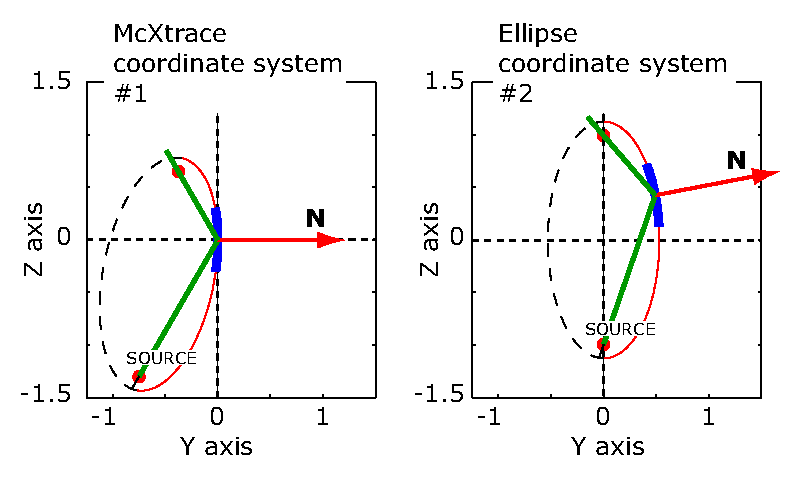
\includegraphics[width=0.95\linewidth]{figures/ellipse.eps}
 \caption{The same image in different coordinate systems.\newline \emph{Left}:
 \emph{McXtrace System} with the y-axis is parallel to the central mirror normal, the z-axis
 is parallel to the central mirror tangent and the origin is at the mirror
 center. \newline
 \emph{Right}: \emph{Ellipse System} with
the z-axis parallel to major axis of ellipse, the y-axis is parallel
to minor axis of ellipse and the origin is at the center of the
ellipse. }\label{fig:Ellipse}
\end{figure}


\subsection{Algorithm}
\begin{enumerate}
\item The photon is generated with a starting point $\bf{S}$ and a direction
$\bf{V}_\textrm{in}$ defined in the \emph{McXtrace} coordinate
system.
\item All calculations are performed in the \emph{Ellipse} coordinate system,
so to proceed the basis is changed to that reference frame.
\item The 2 intersections of the ray with the ellipse are determined.
\item It is checked if any of the intersections are within the area
defined by the mirror.
\item If one of the solutions is valid, the reflection of that ray is
determined.
\item The coordinates of the starting point and direction of the
reflected ray are calculated using the basis of the \emph{McXtrace}
coordinate system.
\end{enumerate}


\section{Reflection of the ray in the mirror}
\begin{figure}[htb!]
\centering
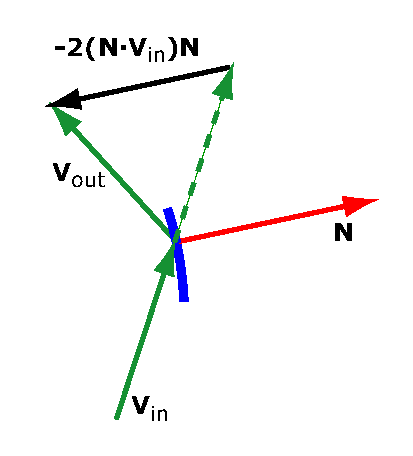
\includegraphics[width=0.3\linewidth]{figures/Dotproduct.eps}
 \caption{The reflection of the unit vector $\bf{V}_\textrm{in}$ in the mirror with the normal unit
 vector $\boldsymbol{{N}}$ is $\boldsymbol{{V}}_\textrm{out} = \boldsymbol{{V}}_\textrm{in} -2(\boldsymbol{{N}}\cdot\boldsymbol{{V}}_\textrm{in})\boldsymbol{{N}}$}\label{fig:dotProduct}
\end{figure}

The tangent and normal to the ellipse $z^2/a^2 + y^2/b^2=1$ at the
point $(Y,Z)$ are found by implicit differentiation: \begin{equation} 
\frac{2z}{a^2} + \frac{2y}{b^2} \,\frac{dy}{dz} = 0\,, \end{equation} so at the
point $(Y,Z)$ the slope of the tangent is $\frac{dy}{dz} =
-\frac{Z\,b^2}{Y\,a^2}$. The slope of the normal is minus the
inverse of the tangent slope, so the coordinates of the mirror
normal are \begin{equation} N_x = 0 \quad N_y = \frac{a^2\,Y}{b^2\,Z} \quad N_z =
1\,. \end{equation} With $\bf{V}_\textrm{in}$ and $\bf{N}$ denoting unit
vectors (direction and normal respectively), the direction of the
reflected ray is calculated as \begin{equation} \boldsymbol{{V}}_\textrm{out} =
\boldsymbol{{V}}_\textrm{in} -2(\boldsymbol{{N}}\cdot\boldsymbol{{V}}_\textrm{in})\boldsymbol{{N}} =
        \left(
      \begin{array}{c}
        V_{\textrm{in}x} - 2(\boldsymbol{{N}}\cdot\boldsymbol{{V}}_\textrm{in})N_x \\
               V_{\textrm{in}y} - 2(\boldsymbol{{N}}\cdot\boldsymbol{{V}}_\textrm{in})N_y \\
                V_{\textrm{in}z} - 2(\boldsymbol{{N}}\cdot\boldsymbol{{V}}_\textrm{in})N_z \\
      \end{array}
    \right)
\end{equation}


\subsection{Mirror reflectivity}
\label{ss:mirrorreflecttable}

At present, the Multilayer\_elliptic Mirror component uses a reflectivity table $reflect$, 
which 1st column is q [$\AA^{-1}$] and from the 2nd column on as the reflectivity $R$ in [0-1]
as function of tabulated energy [$KeV$]. 
An example file, calculated for a particular $Si/W$ multilayer, is provided (\verb+reflectivity.txt+).
User provided reflectivity data files can be parsed by the component.



\section{Mirror\_curved}
\label{mirror-curved}
\index{Mirror!Cylindrically curved mirror}
\component{Mirror\_curved}{System}{\textit{radius,length,width}}{\textit{coating,R0}}{}
 
Models a cylindrical mirror, positioned in the XZ-plane curving towards
positive X. The input parameter \textit{radius} defines the radius of curvature
and the mirror size is given by \textit{length} and \textit{width} where length
and width is along Z and Y respectively. $coating$ and $R0$ are mutually
exclusive. If \textit{R0} is nonzero, it is taken as the reflectivity value,
irrespective of wavelength, whereas coating nominates a file from which to read
values for $f_1$ and $f_2$. See~\cite{NIST-ffast} for definitions. For
elements $Z\in[1,92]$ datafiles are distributed with the McXtrace system that
may be used as: \verb+coating="Rh.txt"+. or \verb+coating="Al.txt"+. 

\section{Mirror\_curved: Cylindrically curved mirror}
\index{Optics!mirror}

\mcdoccomp{optics/Mirror_curved.parms}

Models a cylindrical mirror, positioned in the XZ-plane curving towards
positive X. The input parameter \textit{radius} defines the radius of curvature
and the mirror size is given by \textit{length} and \textit{width} where length
and width is along Z and Y respectively. \textit{coating} and \textit{R0} are mutually
exclusive. If \textit{R0} is nonzero, it is taken as the reflectivity value,
irrespective of wavelength, whereas coating nominates a file from which to read
values for $f_1$ and $f_2$. See~\cite{NIST-ffast} for definitions. For
elements $Z\in[1,92]$ datafiles are distributed with the McXtrace system that
may be used as: \verb+coating="Rh.txt"+. or \verb+coating="Al.txt"+. 

This component is scheduled to be merged with \texttt{Mirror\_parabolic} and \texttt{Mirror\_elliptic} 

\section{Mirror\_parabolic: Mirror with a parabolic curvature profile.}
\index{Optics!mirror}

\mcdoccomp{Mirror_parabolic.parms}

This component is scheduled to be merged with \texttt{Mirror\_elliptic}

\section{Mirror\_elliptic: Mirror with a elliptic curvature profile.}
\index{Optics!mirror}

\mcdoccomp{Mirror_elliptic.parms}

This component is scheduled to be merged with \texttt{Mirror\_parabolic}



\section{Multilayer\_elliptic: Elliptically curved mirror coated with a multilayer}
\index{Optics!multilayer, mirror}

\mcdoccomp{optics/Multilayer_elliptic.parms}

doc. pend.


\section{TwinKB\_ML: Side-by-side Kirkpatrick-Baez mirror pair}

\mcdoccomp{optics/TwinKB_ML.parms}

Models a pair of perpendicular, elliptically curved mirrors, known as a Montel-mirror or Side-by-side Kirkpatrick-Baez mirror.


\chapter{Samples}
\index{Library!Components!samples}
\index{Samples|textbf}
\label{c:samples}

This class of components models the sample of the experiment.
This is by far the most challenging part of a neutron scattering
instrument to model. However, for purpose of simulating
instrument performance, details of the samples are rather unimportant,
allowing for simple approximations. On the contrary, for full
virtual experiments it is of importance to have realistic and
detailed sample descriptions. \MCX\ contains both simple and detailed
samples.

An important component class is elastic Bragg scattering from an ideal powder.
The component \textbf{PowderN} models a powder scatterer with reflections
given in an input file. 
The component includes absorption, incoherent scattering, direct beam
transmission and can assume \emph{concentric} shape, i.e. can be used
for modelling sample enviroments.

Next type is Bragg scattering from single crystals. Two types of single crystal exist in \MCX
at present: The \textbf{Perfect\_crystal} and \textbf{Single\_crystal} components.
\textbf{Perfect\_crystal} is in fact most often used as a monchromator crystal. It models a 
crystal where peak broadening is dominated by the Darwin width. Currently it only handles a
single defined reflection. If more than one is wanted this could be
accomplished by using two instances in a \texttt{GROUP} and dynamically choose between
them with a \texttt{WHEN}-statement. For details on the \texttt{GROUP} and \texttt{WHEN} constructs see the
main \MCX user manual~\cite{mcxtracemanual}

Much more general, the component \textbf{Single\_crystal}
is a single crystal sample (with multiple scattering) that allows
the input of an arbitrary unit cell and a list of structure factors, read
from a LAZY / Crystallographica file.
This component also allows anisotropic mosaicity
and $\Delta d/d$ lattice space variation.

Isotropic small-angle scattering is simulated in \textbf{Saxs\_Spheres},
which models scattering from a collection of hard spheres (dilute colloids).
Furthermore, a whole series of sample components modelling various SAXS standard 
sample types are available in the  \texttt{contrib} component library section.

\subsection{Scattering notation}
In sample components, we use a notation common for scattering experiments,
where the wave vector transfer is denoted the {\em scattering vector}
\begin{equation} \label{eq:q-transfer}
\boldsymbol{q} \equiv \boldsymbol{k}_\mathrm{i} - \boldsymbol{k}_\mathrm{f} .
\end{equation}
In analygo, the {\em energy transfer} is given by
\begin{equation} \label{eq:w-transfer}
\hbar \omega \equiv E_\mathrm{i} - E_\mathrm{f} =
\frac{\hbar^2}{2 m_\mathrm{n}} \left( k_\mathrm{i}^2 - k_\mathrm{f}^2 \right) .
\end{equation}

\subsection{Weight transformation in samples; focusing}

Within many samples,
the incident beam is attenuated by scattering and absorption,
so that the illumination varies considerably throughout the sample.
For single crystals, this phenomenon is known as
{\em secondary extinction} \cite{bacon}, but the effect is
important for all samples.
In analytical treatments, attenuation is difficult to deal with,
and is thus often ignored, making a {\em thin sample approximation}.
In Monte Carlo simulations, the beam attenuation
is easily taken care of, as will be shown below.
In the description, we ignore multiple scattering, which is however
 implemented in some sample components.

The sample has an absorption cross section per unit cell of
$\sigma_c^a$ and a scattering cross section per unit cell
of $\sigma_c^s$. The x-ray path length
in the sample before the scattering event is denoted by $l_1$, and
the path length within the sample after the scattering
is denoted by $l_2$, see figure \ref{powderFig}.
We then define the inverse penetration lengths as
$\mu^s = \sigma_c^s / V_c$ and $\mu^a = \sigma_c^a / V_c$, where
$V_c$ is the volume of a unit cell. Physically, the attenuation
along this path follows
\begin{equation}
f_\mathrm{att}(l) = \exp(- l (\mu^s + \mu^a)) ,
\end{equation}
where the normalization $f_\mathrm{att}(0)=1$.

\begin{figure}
  \begin{center}
    \psfrag{l1}{$l_1$}
    \psfrag{l2}{$l_2$}
    \psfrag{lfull}{$l_\mathrm{full}$}
    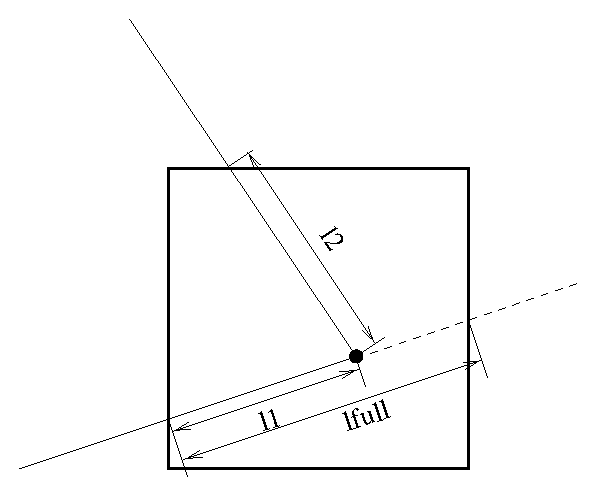
\includegraphics[width=0.6\textwidth]{figures/scatter.eps}
  \end{center}
\caption{The geometry of a scattering event within a powder sample.}
\label{powderFig}
\end{figure}

The probability for a given x-ray to be scattered from within the interval
$[ l_1 ; l_1+dl ]$ will be
\begin{equation}
P(l_1) dl = \mu^s f_\mathrm{att}(l_1) dl ,
\end{equation}
while the probability for a x-ray to be scattered from within
this interval into the solid angle $\Omega$ {\em and}
not being scattered further
or absorbed on the way out of the sample is
\begin{equation}
P(l_1,\Omega) dl d\Omega =
  \mu^s f_\mathrm{att}(l_1) f_\mathrm{att}(l_2) \gamma(\Omega) d\Omega dl ,
\end{equation}
where $\gamma(\Omega)$ is the directional distribution
of the scattered x-rays, and $l_2$ is determined by
Monte Carlo chocies of $l_1$, $\Omega$,
and from the sample geometry, see e.g. figure \ref{powderFig}.

In our Monte-Carlo simulations, we may choose the scattering
parameters by making a Monte-Carlo choice of $l_1$ and $\Omega$
from a distribution different from $P(l_1,\Omega)$.
By doing this, we must adjust $\pi_i$ according to
the probability transformation rule (\ref{probrule}).
If we {\em e.g.}\ choose the scattering depth, $l_1$,
from a flat distribution in $[ 0 ; l_\mathrm{full} ]$,
and choose the directional dependence from $g(\Omega)$,
we have a Monte Carlo probability
\begin{equation}
f(l_1,\Omega) = g(\Omega) / l_\mathrm{full} ,
\end{equation}
$l_\mathrm{full}$ is here the path length through the sample
as taken by a non-scattered neutron (although we here
assume that all simulated x-rays are being scattered).
According to (\ref{probrule}), the x-ray weight factor
is now adjusted by the amount
\begin{equation}     \label{sampleprob}
\pi_i(l_1,\Omega) =
 \mu^s l_\mathrm{full} \exp \left[ - (l_1+l_2) (\mu^a + \mu^s) \right]
  \frac{\gamma(\Omega)}{g(\Omega)} .
\end{equation}

In analogy with the source components, it is possible to define
"interesting" directions for the scattering.
One will then try to focus the scattered x-rays,
choosing a $g(\Omega)$, which peaks around these directions.
To do this, one uses (\ref{sampleprob}), where the
fraction $\gamma(\Omega)/g(\Omega)$ corrects for the focusing.
One must choose a proper distribution so that
$g(\Omega) > 0$ in every interesting direction. If this is not the
case, the Monte Carlo simulation gives incorrect results.
All samples have been constructed with a focusing
and a non-focusing option.


\subsection{Future development of sample components}
There is still room for much more development of functionality in
\MCX\ samples.

%\section{V\_sample: An incoherent scatterer, the V-sample}
\label{s:v_sample}
\index{Samples!Incoherent isotropic scatterer (Vanadium)}
\index{Incoherent elastic scattering}

\component{V\_sample}{System}{$r_{\rm i}$, $r_{\rm o}$, $h$, $r_{\rm foc}$, $x_{\rm target}$, $y_{\rm target}$, $z_{\rm target}$}{$w_x$, $h_y$, $t_z$, $w_{\rm focus}, h_{\rm focus}$, $w_{\rm foc, angle}$, $h_{\rm foc, angle}$, \\ $\sigma_{\rm abs}$, $\sigma_{\rm inc}$, $V_0$, $f_{\rm pack}$, target\_index}{validated}

A sample with incoherent scattering, e.g. vanadium, is frequently used for
calibration purposes, as this gives an isotropic, elastically scattered beam.

The component {\bf V\_sample}
has {\em only} absorption and incoherent elastic scattering.
For the sample geometry, we default use a
hollow cylinder (which has the solid cylinder as a limiting case).
The sample dimensions are: Inner radius $r_{\rm i}$,
outer radius $r_{\rm o}$, and height $h$, see figure \ref{f:v-sample}.
\begin{figure}
  \begin{center}
    \psfrag{ri}{$r_i$}
    \psfrag{ro}{$r_o$}
    \psfrag{h}{$h$}
    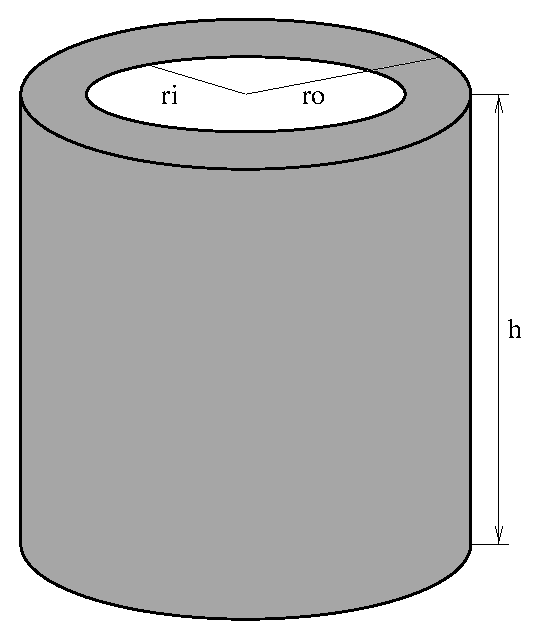
\includegraphics[width=0.3\textwidth]{figures/vsample.eps}
  \end{center}
\caption{The geometry of the hollow-cylinder vanadium sample.}
\label{f:v-sample}
\end{figure}

Alternatively, the sample geometry can be made rectangular
by specifying the width, $w_x$, the height, $h_y$, and the thickness, $t_z$.

The incoherent and absorption cross sections for V are default
for the component. For other choices, the
parameters $\sigma_{\rm inc}$, $\sigma_{\rm abs}$,
and the unit cell volume $V_0$ should be specified.
For a loosely packed sample, also the packing factor, $f_{\rm pack}$
can be specified (default value of 1).

\subsection{Physics and algorithm}

The incoherent scattering gives
a uniform angular distribution of the scattered
neutrons from each nucleus: $\gamma(\Omega) = 1/4\pi$.
For the focusing we choose to have a uniform distribution on
a target sphere of radius $r_{\rm foc}$, at the position
$(x_{\rm target},y_{\rm target},z_{\rm target})$
in the local coordinate system.
This gives an angular distribution (in a small angle approximation)
of
\begin{equation}
g(\Omega) = \frac{1}{4\pi}
  \frac{x_{\rm t}^2+y_{\rm t}^2+z_{\rm t}^2}{(\pi r_{\rm t}^2)}.
\end{equation}

The focusing can alternatively be performed on a rectangle with dimensions
$w_{\rm focus}$, $h_{\rm focus}$, or uniformly in angular space
(in a small-angle approximation),
using $w_{\rm foc, angle}$, $h_{\rm foc, angle}$.
The focusing location can be picked to be a downstream component by
specifying \\
\verb+target_index+.

When calculating the neutron path length within
the cylinder, the kernel function \\
\verb+cylinder_intersect+
is used twice, once for the outer radius and once
for the inner radius.

Multiple scattering is not included in this component. To obtain
intensities similar to real measured ones, we therefore do not
take attenuation from scattering into account for the outgoing
neutron ray.

\subsection{Remark on functionality}
When simulating a realistic incoherent hollow cylinder sample
one finds that  the resulting direction dependence
of the scattered intensity is {\em not} isotropic.
This is explained by the variation of attenuation with
scattering angle.
One test result is shown in the instrument example chapter of the \MCS User Manual.

The \verb+Samples_vanadium+ and \verb+Samples_incoherent+ test/example instruments exist in the distribution for this component.
         \newpage
%\section{Tunneling\_sample: An incoherent inelastic scatterer}
\label{s:Tunneling_sample}
\index{Samples!Incoherent inelastic scatterer}
\index{Incoherent inelastic scattering}

\component{Tunneling\_sample}{System}{$r_{\rm i}$, $r_{\rm o}$, $h$, $r_{\rm foc}$, $x_{\rm target}$, $y_{\rm target}$, $z_{\rm target}$}{$w_x$, $h_y$, $t_z$, $w_{\rm focus}, h_{\rm focus}$, $w_{\rm foc, angle}$, $h_{\rm foc, angle}$, $\sigma_{\rm abs}$, $\sigma_{\rm inc}$, $V_0$, $f_{\rm pack}$, $f_{\rm QE}$, $f_{\rm tun}$, $\Gamma$, $E_{\rm tun}$, target\_index}{not validated}

The component {\bf Tunneling\_sample}
displays incoherent inelastic scattering as found in a number of systems, {\em e.g.}
containing mobile hydrogen. 

For the sample geometry, we default use a
hollow cylinder (which has the solid cylinder as a limiting case).
The sample dimensions are: Inner radius $r_{\rm i}$,
outer radius $r_{\rm o}$, and height $h$. This geometry is the same as 
the default for {\bf V\_sample}, see figure \ref{f:v-sample}.

As for {\bf V\_sample}, the sample geometry can be made rectangular 
by specifying the width, $w_x$, the height, $h_y$, and the thickness, $t_z$.

Also the focusing properties are the same as for {\bf V\_sample}.
For the focusing is performed as a uniform distribution on
a target sphere of radius $r_{\rm foc}$, at the position
$(x_{\rm target},y_{\rm target},z_{\rm target})$
in the local coordinate system.
The focusing can alternatively be performed on a rectangle with dimensions
$w_{\rm focus}$, $h_{\rm focus}$, or uniformly in angular space
(in a small-angle approximation),
using $w_{\rm foc, angle}$, $h_{\rm foc, angle}$.
The focusing location can be picked to be a downstream component by
specifying \verb+target_index+.

The incoherent and absorption cross sections for V are default
for the component. For other choices, the
parameters $\sigma_{\rm inc}$, $\sigma_{\rm abs}$,
and the unit cell volume $V_0$ should be specified.
For a loosely packed sample, also the packing factor, $f_{\rm pack}$
can be specified (default value of 1).

The inelastic scattering takes place as a quasielastic (Lorentzian)
component, which is chosen with probability $f_{\rm QE}$.
The broadening of the signal is given by $\Gamma$ (HWHM).
In addition, a tunneling signal is present with a probability of $f_{\rm tun}$ 
and a tunneling energy of $\pm E_{\rm tun}$. 
The tunneling peaks are weighted by the usual factor $k_{\rm f}/k_{\rm i}$.

The total scattering cross section is given by
\begin{eqnarray}
\lefteqn{\frac{d^2\sigma}{d\Omega dE_{\rm f}}(q,\omega) = \frac{\sigma_{\rm inc}}{4\pi}
\times \left\{ (1-f_{\rm QE}-f_{\rm inel}) \delta(\hbar \omega) \right. }  \\
 &+& f_{\rm QE} \frac{\Gamma}{(\hbar\omega)^2+\Gamma^2}
 + \left.\frac{f_{\rm inel}}{2} \frac{k_{\rm f}}{f_{\rm i}} 
   \left[\delta(\hbar\omega-E_{\rm tun}) + \delta(\hbar\omega+E_{\rm tun}) \right] \right\} \nonumber
\end{eqnarray}

The component takes care that 
$f_{\rm QE} + f_{\rm tun} \leq 1$, otherwise an error is returned.

The component accounts for absorption, 
but not multiple scattering. To obtain
intensities similar to real measured ones, we therefore do not 
take attenuation from scattering into account for the outgoing
neutron ray.

        \newpage
\section{Absorption\_sample: An absorption phantom}
\index{Samples!Absorption}
\index{Tomography}
\label{absorption_sample}
\mcdoccomp{samples/Absorption_sample.parms}

This component models an absorption phantom with a single inclusion in surrounding material. It is intended use
is for tomographic imaging simulations.

%describe data format
 
\newpage
\section{Saxs\_spheres: A model of dilute hard spheres in solution for SAXS-use}
\index{Samples!SAXS}
\label{saxs_spheres}

\mcdoccomp{samples/Saxs_spheres.parms}

Pending documetation
 \newpage
\section{PowderN: A general powder sample}
\index{Samples!Powder, multiple diffraction line}
\index{Diffraction}
\index{Sample environments}
\index{Concentric components}
\label{powder}

\section{PowderN: A general powder sample}
\index{Samples!Powder, multiple diffraction line}
\index{Diffraction}
\index{Sample environments}
\index{Concentric components}
\label{powder}

\input{samples/PowderN.parms}
%\component{Powder\_N}{System}{$radius$, $thickness$, $h$, $xwidth$, $yheight$, $zdepth$, $\sigma_\mathrm{abs}$,
%  $\sigma_\mathrm{inc}$, $Vc$, $f_\mathrm{pack}$, reflections, format, DW, concentic, and more}{}{}

The powder diffraction component \textbf{PowderN} models a powder sample
with background coming only from incoherent scattering and no
multiple scattering. At the users choice, a given percentage of the incoming
events may be transmitted (attenuated) to model the direct beam. The component can also
assume \emph{concentric} shape, i.e. be used for describing sample environment (cryostat,
sample container etc.). 

The description of the powder comes from a file in one of the standard output formats LAZY, FULLPROF, or CRYSTALLOGRAPHICA.

%A usage example of this component can be found in the \\
%\verb+x-ray site/Tutorial/templateDIFF+ instrument from the \verb+mcgui+.

\subsection{Files formats: powder structures}

Data files of type \verb'lau' and \verb'laz' in the \MCX distribution data directory are self-documented in their header. 
%A list of common powder definition files is available in Table \ref{t:powders-data} (page \pageref{t:powders-data}). They do not need any additional parameters to be used, as in the example:
\begin{verbatim}
  PowderN(<geometry parameters>, filename="Al.laz")
\end{verbatim}
Other column-based file formats may also be imported e.g. with parameters such as:
\begin{verbatim}
  format=Crystallographica
  format=Fullprof
  format={1,2,3,4,0,0,0,0}
\end{verbatim}
In the latter case, the indices define order of columns parameters
multiplicity, lattice spacing, $F^2$, Debye-Waller factor and intrinsic line width.

The column signification may as well explicitely be set in the data file header using any of the lines:
\begin{verbatim}
  #column_j     <index of the multiplicity 'j' column>
  #column_d     <index of the d-spacing 'd' column>
  #column_F2    <index of the squared str. factor '|F|^2' column [b]>
  #column_F     <index of the structure factor norm '|F|' column>
  #column_DW    <index of the Debye-Waller factor 'DW' column>
  #column_Dd    <index of the relative line width Delta_d/d 'Dd' column>
  #column_inv2d <index of the 1/2d=sin(theta)/lambda 'inv2d' column>
  #column_q     <index of the scattering wavevector 'q' column>
\end{verbatim}

Other component parameters may as well be specified in the data file
header with lines e.g.:
\begin{verbatim}
  #V_rho        <value of atom number density [at/Angs^3]>
  #Vc           <value of unit cell volume Vc [Angs^3]>
  #sigma_abs    <value of Absorption cross section [barns]>
  #sigma_inc    <value of Incoherent cross section [barns]>
  #Debye_Waller <value of Debye-Waller factor DW>
  #Delta_d/d    <value of Detla_d/d width for all lines>
  #density      <value of material density [g/cm^3]>
  #weight       <value of material molar weight [g/mol]>
  #nb_atoms     <value of number of atoms per unit cell>
\end{verbatim}

Further details on file formats are available in the \texttt{mxdoc} page
of the component.

\subsection{Geometry, physical properties, concentricity}
The sample has the shape of a solid cylinder, radius $r$ and height $h$ or a box-shaped
sample of size $xwidth$ x $yheight$ x $zdepth$. At the users choice, an inner 'hollow' can be
specified using the parameter $thickness$. 


%As the Isotropic\_Sqw component~\ref{s:isotropic-sqw}, 
PowderN can assume a \emph{concentric} shape, i.e.
can contain other components inside the inner hollow. To allow this, two almost identical copies
of the PowderN components must be set up \emph{around} the internal component(s), for example:


\begin{verbatim}
COMPONENT Cryo = PowderN(reflections="Al.laz", radius = 0.01, thickness = 0.001,
                          concentric = 1)
AT (0,0,0) RELATIVE Somewhere

COMPONENT Sample = some_other_component(with geometry FULLY enclosed in the hollow)
AT (0,0,0) RELATIVE Somewhere

COMPONENT Cryo2 = COPY(Cryo)(concentric = 0)
AT (0,0,0) RELATIVE Somewhere
\end{verbatim}

As outlined, the first instance of PowderN \emph{must} have \texttt{concentric = 1} and the second instance \emph{must}
have \textt{concentric = 0}. Furthermore, the component(s) inside the hollow \emph{must} have a geometry which can
be fully contained inside the hollow.


In addition to the coherent scattering specified in the \verb+reflections+ file, absorption- and incoherent 
cross sections can be given using the input parameters $\sigma_c^a$ and $\sigma_i^s$.


The Bragg scattering from the powder,
$\sigma_c^s$ is calculated from the input file, with the parameters
$Q$, $|F(Q)|^2$, and $j$ for the scattering vector, structure factor, and
multiplicity, respectively. The volume of the unit cell is denoted $Vc$,
while the sample packing factor is $f_\mathrm{pack}$.


%Further, the incoherent scattering is only taken into account
%by the attenuation of the beam, given by (\ref{e:attenu})
%and $\sigma_c^a$.
%The incoherently scattered x-rays are not
%propagated through to the detector, but rather not generated at all.

Focusing is performed by only scattering into one angular
interval, $d\phi$ of the Debye-Scherrer circle. The center of this
interval is located at the point where the Debye-Scherrer circle
intersects the half-plane defined by the initial velocity, $\boldsymbol{v}_\mathrm{i}$,
and a user-specified vector, $\boldsymbol{f}$.

%The input parameters for this component are
%
%\begin{quote}\begin{tabular}{ccl}
%$r$ & m & Radius of cylinder \\
%$h$ & m & Height of cylinder \\
%$\sigma_c^a$ & fm$^2$ & Absorption cross section per unit cell (at 2200 m/s) \\
%$\sigma_{i,c}^s$ & (fm)$^2$ & Incoherent scattering cross section per unit cell \\
%$\rho'/\rho$ & 1 & Packing factor \\
%$V_c$ & \AA$^3$ & Volume of unit cell \\
%$\boldsymbol{Q}$ & \AA$^{-1}$ & The reciprocal lattice vector under consideration \\
%$|F(\textbf{Q}_j)|^2$ & (fm)$^2$ &
% Structure factor \\
%$j$ & 1 & Multiplicity of reflection \\
%$\exp(-2W)$ & 1 & Debye-Waller factor \\
%$d\phi$ & deg & Angular interval of focusing \\
%$f_x$ & m & \\
%$f_y$ & m & Focusing vector\\
%$f_z$ & m & \\
%\end{tabular}\end{quote}

\subsection{Powder scattering}
An ideal powder sample consists of many small
crystallites, although each crystallite is sufficiently
large not to cause measurable size broadening.
The orientation of the crystallites is evenly distributed,
and there is thus always a large number of
crystallites oriented to fulfill the Bragg condition
\begin{equation}   \label{Bragg}
n \lambda = 2 d \sin \theta ,
\end{equation}
where $n$ is the order of the scattering (an integer), $\lambda$
is the x-ray wavelength, $d$ is the lattice spacing of the sample,
and $2 \theta$ is the scattering angle, see figure \ref{coneFig}.
As all crystal orientations
are realised in a powder sample, the x-rays are scattered within a
{\em Debye-Scherrer cone} of opening angle $4 \theta$ \cite{bacon}.

\begin{figure}
  \begin{center}
    \psfrag{2theta}[c][c]{$2\theta$}
    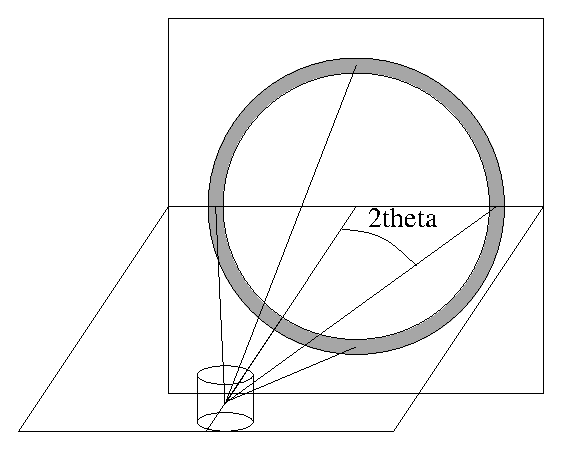
\includegraphics[width=0.6\textwidth]{figures/powder.eps}
  \end{center}
\caption{The scattering geometry of a powder sample showing part of the
Debye-Scherrer cone (solid lines) and the Debye-Scherrer circle (grey).}
\label{coneFig}
\end{figure}

Equation (\ref{Bragg}) may be cast into the form
\begin{equation}
|\boldsymbol{Q}| = 2 |\boldsymbol{k}| \sin \theta ,
\end{equation}
where \textbf{Q} is a vector of the reciprocal lattice, and \textbf{k} is
the wave vector of the x-ray. It is seen that only
reciprocal vectors fulfilling $|\boldsymbol{Q}| < 2 |\boldsymbol{k}|$
contribute to the scattering.
For a complete treatment of the powder sample, one needs to take
into account all these \textbf{Q}-values, since each of them contribute
to the attenuation.

The strength of the Bragg reflections is given by their structure factors
\begin{equation}
 \left| \sum_j b_j \exp(\boldsymbol{R}_j \cdot \boldsymbol{Q}) \right|^2 ,
\end{equation}
where the sum runs over all atoms in one unit cell. This structure factor is
non-zero only when $Q$ equals a reciprocal lattice vector.

The textbook expression for the scattering cross section
corresponding to one Debye-Scherrer cone reads \cite[ch.3.6]{squires}, with $V=N V_0$ being the total sample volume:
\begin{equation}
\sigma_\mathrm{cone}
  = \frac{V}{V_0^2} \frac{\lambda^3}{4 \sin \theta} \sum_Q |F(Q)|^2 .
\end{equation}
For our purpose, this expression should be changed slightly.
Firstly, the sum over structure factors for a particular $Q$ is replaced
by the sum over essentially different reflections multiplied by their
multiplicity, $j$. Then, a finite packing factor, $f$, is defined for the powder,
and finally, the Debye-Waller factor is multiplied on the elastic cross section
to take lattice vibrations into account (no inelastic background is simulated,
however). We then reach
\begin{eqnarray}
\sigma_\mathrm{cone, Q}
 & = & j_Q f \exp(-2W) \frac{V}{V_0^2} \frac{\lambda^3}{4 \sin \theta} |F(Q)|^2 \\
 & = & f \exp(-2W) \frac{N}{V_0} \frac{4\pi^3}{k^2} \frac{j_Q |F(Q)|^2}{Q}
\end{eqnarray}
in the thin sample approximation. For samples of finite thickness, the
beam is being attenuated by the attenuation coefficient
\begin{equation}
\label{e:attenu}
\mu_\mathrm{Q} = \sigma_\mathrm{cone,Q} / V .
\end{equation}
For calibration it may be useful to consider the total intensity
scattered into a detector of effective height $h$, covering only
one reflection \cite[ch.3.6]{squires}.
A cut though the Debye-Scherrer cone perpendicular to its axis
is a circle. At the distance $r$ from the sample, the radius of this
circle is $r \sin(2\theta)$. Thus, the detector (in a small angle
approximation) counts a fraction $h / (2 \pi r \sin(2 \theta))$
of the scattered x-rays, giving a resulting count intensity:
\begin{equation}
I = \Psi \sigma_\mathrm{cone,Q} \frac{h}{2 \pi r \sin(2\theta)} ,
\end{equation}
where $\Psi$ is the flux at the sample position.

For clarity we repeat the meaning and unit of the symbols:
%
\begin{quote}\begin{tabular}{ccl}
$\Psi$ & s$^{-1}$m$^{-2}$ & Incoming intensity of x-rays \\
$I$    & s$^{-1}$ & Detected intensity of x-rays \\
$h$    & m        & Height of detector \\
$r$    & m        & Distance from sample to detector \\
$f$    & 1        & Packing factor of the powder \\
$j$    & 1        & Multiplicity of the reflection \\
$V_0$  & m$^{3}$  & Volume of unit cell\\
$|F(\boldsymbol{Q})|^2$ & m$^2$  & Structure factor \\
$\exp(-2W)$ & 1  & Debye-Waller factor \\
$\mu_\mathrm{Q}$ & m$^{-1}$ & Linear attenuation factor due to scattering from
one powder line. \\
\end{tabular}\end{quote}
%
%Often, one defines the {\em scattering power} as
%\begin{equation}
%Q \equiv N^2 \frac{|F(\boldsymbol{Q})|^2 \lambda^3}{V \sin(2\theta)}
% = N_c^2 V \frac{\rho'}{\rho} \frac{|F(\boldsymbol{Q})|^2 \lambda^3}{\sin(2\theta)} ,
%\end{equation}
%where $N$ is the number of unit cells.

A powder sample will in general have several allowed reflections
$\boldsymbol{Q}_j$, which will all contribute to the attenuation.
These reflections will have different values of
$|F(\boldsymbol{Q}_j)|^2$ (and hence of $Q_j$), $j_j$, $\exp(-2W_j)$,
and $\theta_j$.
The total attenuation through the sample due to scattering is given by
$\mu^s = \mu_\mathrm{inc}^s + \sum_j \mu^s_j $,
where $\mu_\mathrm{inc}^s$ represents the incoherent scattering.

\subsection{Algorithm}
The algorithm of \textbf{PowderN} can be summarized as
\begin{itemize}
\item Check if the x-ray intersects the sample (otherwise ignore
the following).
\item Calculate the attenuation coefficients for scattering and absorption.
\item Perform Monte Carlo choices to determine the scattering position,
scattering type (coherent/incoherent), and the outgoing direction.
\item Perform the necessary weight factor transformation.
\end{itemize}

%\subsection{Calculating the weight factor}

%\component{Powder\_N}{System}{$radius$, $thickness$, $h$, $xwidth$, $yheight$, $zdepth$, $\sigma_\mathrm{abs}$,
%  $\sigma_\mathrm{inc}$, $Vc$, $f_\mathrm{pack}$, reflections, format, DW, concentic, and more}{}{}

The powder diffraction component \textbf{PowderN} models a powder sample
with background coming only from incoherent scattering and no
multiple scattering. At the users choice, a given percentage of the incoming
events may be transmitted (attenuated) to model the direct beam. The component can also
assume \emph{concentric} shape, i.e. be used for describing sample environment (cryostat,
sample container etc.). 

The description of the powder comes from a file in one of the standard output formats LAZY, FULLPROF, or CRYSTALLOGRAPHICA.

%A usage example of this component can be found in the \\
%\verb+x-ray site/Tutorial/templateDIFF+ instrument from the \verb+mcgui+.

\subsection{Files formats: powder structures}

Data files of type \verb'lau' and \verb'laz' in the \MCX distribution data directory are self-documented in their header. 
%A list of common powder definition files is available in Table \ref{t:powders-data} (page \pageref{t:powders-data}). They do not need any additional parameters to be used, as in the example:
\begin{verbatim}
  PowderN(<geometry parameters>, filename="Al.laz")
\end{verbatim}
Other column-based file formats may also be imported e.g. with parameters such as:
\begin{verbatim}
  format=Crystallographica
  format=Fullprof
  format={1,2,3,4,0,0,0,0}
\end{verbatim}
In the latter case, the indices define order of columns parameters
multiplicity, lattice spacing, $F^2$, Debye-Waller factor and intrinsic line width.

The column signification may as well explicitely be set in the data file header using any of the lines:
\begin{verbatim}
  #column_j     <index of the multiplicity 'j' column>
  #column_d     <index of the d-spacing 'd' column>
  #column_F2    <index of the squared str. factor '|F|^2' column [b]>
  #column_F     <index of the structure factor norm '|F|' column>
  #column_DW    <index of the Debye-Waller factor 'DW' column>
  #column_Dd    <index of the relative line width Delta_d/d 'Dd' column>
  #column_inv2d <index of the 1/2d=sin(theta)/lambda 'inv2d' column>
  #column_q     <index of the scattering wavevector 'q' column>
\end{verbatim}

Other component parameters may as well be specified in the data file
header with lines e.g.:
\begin{verbatim}
  #V_rho        <value of atom number density [at/Angs^3]>
  #Vc           <value of unit cell volume Vc [Angs^3]>
  #sigma_abs    <value of Absorption cross section [barns]>
  #sigma_inc    <value of Incoherent cross section [barns]>
  #Debye_Waller <value of Debye-Waller factor DW>
  #Delta_d/d    <value of Detla_d/d width for all lines>
  #density      <value of material density [g/cm^3]>
  #weight       <value of material molar weight [g/mol]>
  #nb_atoms     <value of number of atoms per unit cell>
\end{verbatim}

Further details on file formats are available in the \texttt{mxdoc} page
of the component.

\subsection{Geometry, physical properties, concentricity}
The sample has the shape of a solid cylinder, radius $r$ and height $h$ or a box-shaped
sample of size $xwidth$ x $yheight$ x $zdepth$. At the users choice, an inner 'hollow' can be
specified using the parameter $thickness$. 


%As the Isotropic\_Sqw component~\ref{s:isotropic-sqw}, 
PowderN can assume a \emph{concentric} shape, i.e.
can contain other components inside the inner hollow. To allow this, two almost identical copies
of the PowderN components must be set up \emph{around} the internal component(s), for example:


\begin{verbatim}
COMPONENT Cryo = PowderN(reflections="Al.laz", radius = 0.01, thickness = 0.001,
                          concentric = 1)
AT (0,0,0) RELATIVE Somewhere

COMPONENT Sample = some_other_component(with geometry FULLY enclosed in the hollow)
AT (0,0,0) RELATIVE Somewhere

COMPONENT Cryo2 = COPY(Cryo)(concentric = 0)
AT (0,0,0) RELATIVE Somewhere
\end{verbatim}

As outlined, the first instance of PowderN \emph{must} have \texttt{concentric = 1} and the second instance \emph{must}
have \textt{concentric = 0}. Furthermore, the component(s) inside the hollow \emph{must} have a geometry which can
be fully contained inside the hollow.


In addition to the coherent scattering specified in the \verb+reflections+ file, absorption- and incoherent 
cross sections can be given using the input parameters $\sigma_c^a$ and $\sigma_i^s$.


The Bragg scattering from the powder,
$\sigma_c^s$ is calculated from the input file, with the parameters
$Q$, $|F(Q)|^2$, and $j$ for the scattering vector, structure factor, and
multiplicity, respectively. The volume of the unit cell is denoted $Vc$,
while the sample packing factor is $f_\mathrm{pack}$.


%Further, the incoherent scattering is only taken into account
%by the attenuation of the beam, given by (\ref{e:attenu})
%and $\sigma_c^a$.
%The incoherently scattered x-rays are not
%propagated through to the detector, but rather not generated at all.

Focusing is performed by only scattering into one angular
interval, $d\phi$ of the Debye-Scherrer circle. The center of this
interval is located at the point where the Debye-Scherrer circle
intersects the half-plane defined by the initial velocity, $\boldsymbol{v}_\mathrm{i}$,
and a user-specified vector, $\boldsymbol{f}$.

%The input parameters for this component are
%
%\begin{quote}\begin{tabular}{ccl}
%$r$ & m & Radius of cylinder \\
%$h$ & m & Height of cylinder \\
%$\sigma_c^a$ & fm$^2$ & Absorption cross section per unit cell (at 2200 m/s) \\
%$\sigma_{i,c}^s$ & (fm)$^2$ & Incoherent scattering cross section per unit cell \\
%$\rho'/\rho$ & 1 & Packing factor \\
%$V_c$ & \AA$^3$ & Volume of unit cell \\
%$\boldsymbol{Q}$ & \AA$^{-1}$ & The reciprocal lattice vector under consideration \\
%$|F(\textbf{Q}_j)|^2$ & (fm)$^2$ &
% Structure factor \\
%$j$ & 1 & Multiplicity of reflection \\
%$\exp(-2W)$ & 1 & Debye-Waller factor \\
%$d\phi$ & deg & Angular interval of focusing \\
%$f_x$ & m & \\
%$f_y$ & m & Focusing vector\\
%$f_z$ & m & \\
%\end{tabular}\end{quote}

\subsection{Powder scattering}
An ideal powder sample consists of many small
crystallites, although each crystallite is sufficiently
large not to cause measurable size broadening.
The orientation of the crystallites is evenly distributed,
and there is thus always a large number of
crystallites oriented to fulfill the Bragg condition
\begin{equation}   \label{Bragg}
n \lambda = 2 d \sin \theta ,
\end{equation}
where $n$ is the order of the scattering (an integer), $\lambda$
is the x-ray wavelength, $d$ is the lattice spacing of the sample,
and $2 \theta$ is the scattering angle, see figure \ref{coneFig}.
As all crystal orientations
are realised in a powder sample, the x-rays are scattered within a
{\em Debye-Scherrer cone} of opening angle $4 \theta$ \cite{bacon}.

\begin{figure}
  \begin{center}
    \psfrag{2theta}[c][c]{$2\theta$}
    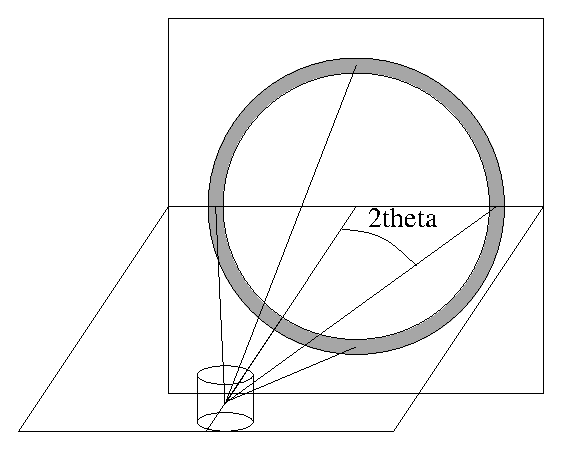
\includegraphics[width=0.6\textwidth]{figures/powder.eps}
  \end{center}
\caption{The scattering geometry of a powder sample showing part of the
Debye-Scherrer cone (solid lines) and the Debye-Scherrer circle (grey).}
\label{coneFig}
\end{figure}

Equation (\ref{Bragg}) may be cast into the form
\begin{equation}
|\boldsymbol{Q}| = 2 |\boldsymbol{k}| \sin \theta ,
\end{equation}
where \textbf{Q} is a vector of the reciprocal lattice, and \textbf{k} is
the wave vector of the x-ray. It is seen that only
reciprocal vectors fulfilling $|\boldsymbol{Q}| < 2 |\boldsymbol{k}|$
contribute to the scattering.
For a complete treatment of the powder sample, one needs to take
into account all these \textbf{Q}-values, since each of them contribute
to the attenuation.

The strength of the Bragg reflections is given by their structure factors
\begin{equation}
 \left| \sum_j b_j \exp(\boldsymbol{R}_j \cdot \boldsymbol{Q}) \right|^2 ,
\end{equation}
where the sum runs over all atoms in one unit cell. This structure factor is
non-zero only when $Q$ equals a reciprocal lattice vector.

The textbook expression for the scattering cross section
corresponding to one Debye-Scherrer cone reads \cite[ch.3.6]{squires}, with $V=N V_0$ being the total sample volume:
\begin{equation}
\sigma_\mathrm{cone}
  = \frac{V}{V_0^2} \frac{\lambda^3}{4 \sin \theta} \sum_Q |F(Q)|^2 .
\end{equation}
For our purpose, this expression should be changed slightly.
Firstly, the sum over structure factors for a particular $Q$ is replaced
by the sum over essentially different reflections multiplied by their
multiplicity, $j$. Then, a finite packing factor, $f$, is defined for the powder,
and finally, the Debye-Waller factor is multiplied on the elastic cross section
to take lattice vibrations into account (no inelastic background is simulated,
however). We then reach
\begin{eqnarray}
\sigma_\mathrm{cone, Q}
 & = & j_Q f \exp(-2W) \frac{V}{V_0^2} \frac{\lambda^3}{4 \sin \theta} |F(Q)|^2 \\
 & = & f \exp(-2W) \frac{N}{V_0} \frac{4\pi^3}{k^2} \frac{j_Q |F(Q)|^2}{Q}
\end{eqnarray}
in the thin sample approximation. For samples of finite thickness, the
beam is being attenuated by the attenuation coefficient
\begin{equation}
\label{e:attenu}
\mu_\mathrm{Q} = \sigma_\mathrm{cone,Q} / V .
\end{equation}
For calibration it may be useful to consider the total intensity
scattered into a detector of effective height $h$, covering only
one reflection \cite[ch.3.6]{squires}.
A cut though the Debye-Scherrer cone perpendicular to its axis
is a circle. At the distance $r$ from the sample, the radius of this
circle is $r \sin(2\theta)$. Thus, the detector (in a small angle
approximation) counts a fraction $h / (2 \pi r \sin(2 \theta))$
of the scattered x-rays, giving a resulting count intensity:
\begin{equation}
I = \Psi \sigma_\mathrm{cone,Q} \frac{h}{2 \pi r \sin(2\theta)} ,
\end{equation}
where $\Psi$ is the flux at the sample position.

For clarity we repeat the meaning and unit of the symbols:
%
\begin{quote}\begin{tabular}{ccl}
$\Psi$ & s$^{-1}$m$^{-2}$ & Incoming intensity of x-rays \\
$I$    & s$^{-1}$ & Detected intensity of x-rays \\
$h$    & m        & Height of detector \\
$r$    & m        & Distance from sample to detector \\
$f$    & 1        & Packing factor of the powder \\
$j$    & 1        & Multiplicity of the reflection \\
$V_0$  & m$^{3}$  & Volume of unit cell\\
$|F(\boldsymbol{Q})|^2$ & m$^2$  & Structure factor \\
$\exp(-2W)$ & 1  & Debye-Waller factor \\
$\mu_\mathrm{Q}$ & m$^{-1}$ & Linear attenuation factor due to scattering from
one powder line. \\
\end{tabular}\end{quote}
%
%Often, one defines the {\em scattering power} as
%\begin{equation}
%Q \equiv N^2 \frac{|F(\boldsymbol{Q})|^2 \lambda^3}{V \sin(2\theta)}
% = N_c^2 V \frac{\rho'}{\rho} \frac{|F(\boldsymbol{Q})|^2 \lambda^3}{\sin(2\theta)} ,
%\end{equation}
%where $N$ is the number of unit cells.

A powder sample will in general have several allowed reflections
$\boldsymbol{Q}_j$, which will all contribute to the attenuation.
These reflections will have different values of
$|F(\boldsymbol{Q}_j)|^2$ (and hence of $Q_j$), $j_j$, $\exp(-2W_j)$,
and $\theta_j$.
The total attenuation through the sample due to scattering is given by
$\mu^s = \mu_\mathrm{inc}^s + \sum_j \mu^s_j $,
where $\mu_\mathrm{inc}^s$ represents the incoherent scattering.

\subsection{Algorithm}
The algorithm of \textbf{PowderN} can be summarized as
\begin{itemize}
\item Check if the x-ray intersects the sample (otherwise ignore
the following).
\item Calculate the attenuation coefficients for scattering and absorption.
\item Perform Monte Carlo choices to determine the scattering position,
scattering type (coherent/incoherent), and the outgoing direction.
\item Perform the necessary weight factor transformation.
\end{itemize}

%\subsection{Calculating the weight factor}
          \newpage
\section{Perfect\_crystal: A Darwin-width domniated single crystal model}

\index{Samples!single crystal, darwin}
\label{perfect_crystal}
\mcdoccomp{samples/Perfect_crystal.parms}

Pedning Further Documetation
\newpage
\section{Single\_crystal: The single crystal component}
\label{s:Single_crystal}
\index{Samples!Single crystal diffraction}
\index{Diffraction}
\index{Incoherent elastic scattering}
\index{Multiple scattering}



\component{Single\_crystal}{Kristian Nielsen}{$x_{width}, y_{height},
z_{thick}$,$\vec a, \vec b, \vec c, \Delta d/d$, mosaic,
reflections}{$\sigma_{abs}, \sigma_{inc}$, ...}{Pending documentation}
%Partially validated, centered.
%Further validation undergoing. Known BUGS: The component is known not to work
%as a Bragg monochromator, likely the problem relates to the internal definition
%of the reciprocal space. Possibly related to this, the model of anistropic
%mosaic is broken - always use a non-zero isotropic mosaic. Also, always use a
%non-zero value of the $\Delta d/d$ parameter.}

%The {\bf Single\_crystal} component models a thick, flat single crystal
%with multiple scattering and absorption with elastic coherent scattering.
%An elastic incoherent background may also be simulated.
%It may be used to describe samples for diffraction,
%but also for accurate monochromator descriptions.
%The component is currently under further review. The current documentation is outdated, especially with respect to the model of crystal mosaicity.
%
%The input parameters for the component are \textit{xwidth},
%\textit{yheight}, and \textit{zdepth} to define the dimensions of the
%crystal in meters (area is centered); \textit{delta\_d\_d} to give the
%value of $\Delta d/d$ (no unit);
%$(\textit{ax}, \textit{ay}, \textit{az})$, $(\textit{bx}, \textit{by},
%\textit{bz})$, and $(\textit{cx}, \textit{cy}, \textit{cz})$ to define
%the axes of the direct lattice of the crystal (the sides of the unit
%cell) in units of {\AA}ngstr{\o}m; and \textit{reflections}, a string
%giving the name of the file with the list of structure factors to
%consider.
%The mosaic is specified \emph{either} isotropically as
%\textit{mosaic}, \emph{or} anisotropically as \textit{mosaic\_h}
%(rotation around the $Y$ axis), \textit{mosaic\_v} (rotation around the
%$Z$ axis), and \textit{mosaic\_n} (rotation around the $X$ axis); in all
%cases in units of full-width-half-maximum minutes of arc.
%
%Optionally, the absorption cross-section at 2200 m/s and the incoherent
%cross-section may be given as \textit{absorption} and
%\textit{incoherent} (in barns), with default of zero; and
%\textit{p\_transmit} may be assigned a fixed Monte Carlo probability for
%transmission through the crystal without any interaction.
%
%The user must specify a list of reciprocal lattice vectors
%$\boldsymbol{\tau}$ to consider along with their structure factors
%$|F_{\boldsymbol{\tau}}|^2$. The user must also specify the coordinates
%(in direct space) of the unit cell axes $\boldsymbol{a}$,
%$\boldsymbol{b}$, and $\boldsymbol{c}$, from which the reciprocal lattice
%will be computed. See section \ref{s:Single_crystal_implement} for file format specifications.
%
%In addition to coherent scattering, {\bf Single\_crystal} also
%handles incoherent scattering and absorption. The incoherent scattering
%cross-section is supplied by the user as a constant
%$\sigma_{\rm inc}$. The absorption cross-section is supplied by the user at
%2200~m/s, so the actual cross-section for a neutron of velocity $v$ is
%$\sigma_{\rm abs} = \sigma_{2200} \frac{\rm 2200~m/s}{v}$.
%
%\subsection{The physical model}
%
%The textbook expression for the scattering cross-section of a crystal
%is~\cite[ch.3]{squires}:
%\begin{equation}
%\label{eq:sigma_coh_el}
%\left(\frac{d\sigma}{d\Omega}\right)_{\rm coh.el.} =
%        N\frac{(2\pi)^3}{V_0}\sum_{\boldsymbol{\tau}}
%        \delta(\boldsymbol{\tau} - \boldsymbol{\kappa})|F_{\boldsymbol{\tau}}|^2
%\end{equation}
%Here $|F_{\boldsymbol{\tau}}|^2$ is the structure factor
%(defined in section~\ref{powder}), $N$ is the
%number of unit cells, $V_0$ is the volume of an
%individual unit cell, and $\boldsymbol{\kappa} (= {\bf k}_i - {\bf k}_f)$
%is the scattering vector. $\delta(\boldsymbol{x})$ is a 3-dimensional delta
%function in reciprocal space,
%so for given incoming wave vector ${\bf k}_i$ and lattice vector
%${\boldsymbol{\tau}}$, only a single final wave vector ${\bf k}_f$ is allowed.
%In general, this wavevector will not fulfill the conditions for elastic
%scattering $(k_f = k_i)$.
%In a real crystal, however, reflections are not perfectly sharp. Because
%of imperfection and finite-size effects, there will be a small region
%around $\boldsymbol{\tau}$ in reciprocal space of possible scattering vectors.
%
%{\bf Single\_crystal} simulates a crystal with a mosaic spread
%$\eta$ and a lattice plane spacing uncertainty $\Delta d/d$. In such
%crystals the reflections will not be completely sharp;
%there will be a small region around each reciprocal lattice point of the
%crystal that contains valid scattering vectors.
%
%We model the mosaicity and $\Delta d/d$ of the crystal with
%3-dimensional Gaussian functions in reciprocal space (see
%figure~\ref{fig:crystal-reciprocal-space}). Two of the axes of the
%Gaussian are perpendicular to the reciprocal lattice vector $\boldsymbol{\tau}$ and model
%the mosaicity. The third one is parallel to $\boldsymbol{\tau}$ and models
%$\Delta d/d$. We assume that the
%mosaicity is small so that the possible directions of the scattering
%vector may be approximated with a Gaussian in rectangular
%coordinates.
%\begin{figure}[t]
%  \begin{center}
%    \psfrag{ki}[r][r]{$\boldsymbol{k}_{\rm i}$}
%    \psfrag{kf}[l][l]{$\boldsymbol{k}_{\rm f}$}
%    \psfrag{tau}[r][r]{$\boldsymbol{\tau}$}
%    \psfrag{mosaic}[l][l]{$\eta$}
%    \psfrag{del-d-d}[l][l]{$\Delta d/d$}
%    \psfrag{Ewald}[l][l]{Ewald}
%    \psfrag{Sphere}[l][l]{Sphere}
%    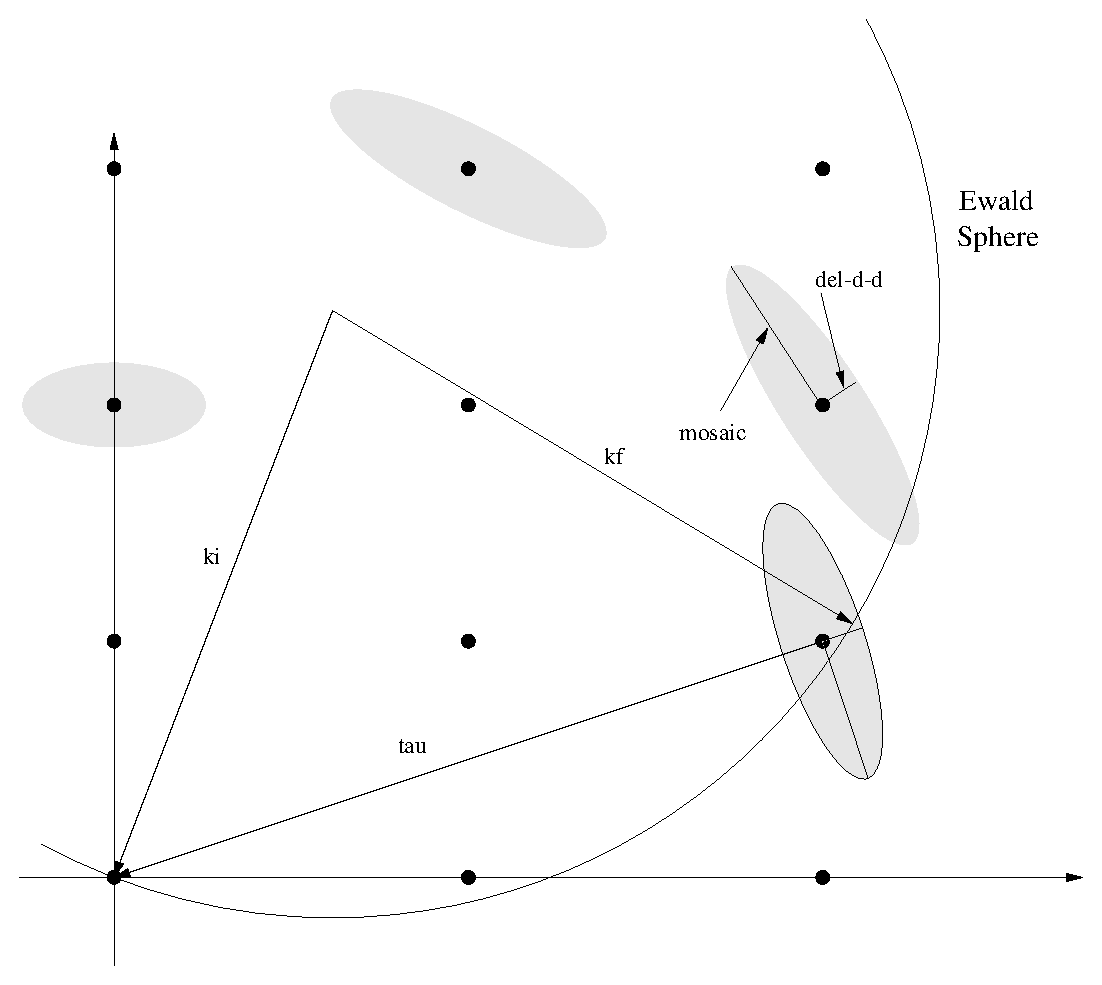
\includegraphics[width=0.7\textwidth]{figures/recip_space3.eps}
%  \end{center}
%\caption{Ewald sphere construction for a single neutron showing the
%    Gaussian broadening of reciprocal lattice points in their local
%    coordinate system.}
%\label{fig:crystal-reciprocal-space}
%\end{figure}
%
%If the mosaic is isotropic (the same in all directions), the two
%Gaussian axes perpendicular to $\boldsymbol{\tau}$ are simply arbitrary
%normal vectors of equal length given by the mosaic. But if the mosaic
%is anisotropic, the two perpendicular axes will in general be different
%for each scattering vector. In the absence of anything better,
%{\bf Single\_crystal} uses a model which is at least mathematically
%plausible and which works as expected in the two common cases:
%(1)~isotropic mosaic, and (2)~two mosaic directions (``horizontal and
%vertical mosaic'') perpendicular to a scattering vector.
%
%The basis for the model is a three-dimensional Gaussian distribution in
%Euler angles giving the orientation probability distribution for the
%micro-crystals; that is, the misorientation is given by small rotations
%around the $X$, $Y$, and $Z$ axes, with the rotation angles having (in
%general different) Gaussian probability distributions. For given
%scattering vector $\boldsymbol{\tau}$, a rotation of the micro-crystals
%around an axis parallel to $\boldsymbol{\tau}$ has no effect on the
%direction of the scattering vector. Suppose we form the intersection
%between the three-dimensional Gaussian in Euler angles and a plane
%through the origin perpendicular to $\boldsymbol{\tau}$. This gives a
%two-dimensional Gaussian, say with axes defined by unit vectors
%$\boldsymbol{g}_1$ and $\boldsymbol{g}_2$ and mosaic widths $\eta_1$ and
%$\eta_2$.
%
%We now let the mosaic for $\boldsymbol{\tau}$ be defined by rotations
%around $\boldsymbol{g}_1$ and $\boldsymbol{g}_2$ with angles having
%Gaussian distributions of widths $\eta_1$ and $\eta_2$. Since
%$\boldsymbol{g}_1$, $\boldsymbol{g}_2$, and $\boldsymbol{\tau}$ are
%perpendicular, a small rotation of $\boldsymbol{\tau}$ around
%$\boldsymbol{g}_1$ will change $\boldsymbol{\tau}$ in the direction of
%$\boldsymbol{g}_2$. The two axes of the Gaussian mosaic in reciprocal
%space that are perpendicular to $\boldsymbol{\tau}$ will thus be given
%by $\tau\eta_2\boldsymbol{g}_1$ and $\tau\eta_1\boldsymbol{g}_2$.
%
%We now derive a quantitative expression for the scattering cross-section
%of the crystal in the model. For this, we introduce a \emph{local
%  coordinate system} for each reciprocal lattice point
%$\boldsymbol{\tau}$ and use $\boldsymbol{x}$ for vectors written in local
%coordinates. The origin is $\boldsymbol{\tau}$, the first axis
%is parallel to $\boldsymbol{\tau}$ and the other two axes are
%perpendicular to $\boldsymbol{\tau}$. In the local coordinate system,
%the 3-dimensional Gaussian is given by
%\begin{equation}
%  \label{eq:crystal-gauss-1}
%  G(x_1,x_2,x_3) = \frac{1}{(\sqrt{2\pi})^3}\frac{1}{\sigma_1\sigma_2\sigma_3}
%  e^{-\frac{1}{2}(\frac{x_1^2}{\sigma_1^2} +
%  \frac{x_2^2}{\sigma_2^2} + \frac{x_3^2}{\sigma_3^2})}
%\end{equation}
%The axes of the Gaussian are $\sigma_1 = \tau\Delta d/d$ and $\sigma_2 =
%\sigma_3 = \eta\tau$. Here we used the assumption that $\eta$ is small,
%so that $\tan\eta \approx \eta$ (with $\eta$ given in radians).  By
%introducing the diagonal matrix
%$$
%D = \left(
%  \begin{array}[c]{ccc}
%    \frac{1}{2}\sigma_1^2 & 0 & 0 \\
%    0 & \frac{1}{2}\sigma_2^2 & 0 \\
%    0 & 0 & \frac{1}{2}\sigma_3^2
%  \end{array}\right)
%$$
%equation~(\ref{eq:crystal-gauss-1}) can be written as
%\begin{equation}
%  G(\boldsymbol{x}) =
%  \frac{1}{(\sqrt{2\pi})^3}\frac{1}{\sigma_1\sigma_2\sigma_3}
%  e^{-\boldsymbol{x}^{\rm T} D \boldsymbol{x}}
%\end{equation}
%again with $\boldsymbol{x}=(x_1,x_2,x_3)$ written in local coordinates.
%
%To get an expression in the coordinates of the reciprocal lattice of the
%crystal, we introduce a matrix $U$ such that if $\boldsymbol{y} =
%(y_1,y_2,y_3)$ are the global coordinates of a point in the crystal
%reciprocal lattice, then $U(\boldsymbol{y} + \boldsymbol{\tau})$ are the
%coordinates in the local coordinate system for $\boldsymbol{\tau}$. The
%matrix $U$ is given by
%$$ U^{\rm T} = (\hat{u}_1, \hat{u}_2, \hat{u}_3), $$
%where $\hat{u}_1$, $\hat{u}_2$, and $\hat{u}_3$ are the axes of the
%local coordinate system, written in the global coordinates of the
%reciprocal lattice. Thus
%$\hat{u}_1 = \boldsymbol{\tau}/\tau$,  and $\hat{u}_2$ and $\hat{u}_3$ are
%unit vectors perpendicular to $\hat{u}_1$ and to each other.
%The matrix $U$ is unitarian, that is
%$U^{-1} = U^{\rm T}$. The translation between global and local
%coordinates is
%$$ \boldsymbol{x} = U(\boldsymbol{y} + \boldsymbol{\tau}) \qquad
%   \boldsymbol{y} = U^{\rm T} \boldsymbol{x} - \boldsymbol{\tau} $$
%
%The expression for the 3-dimensional Gaussian in global coordinates is
%\begin{equation}
%  G(\boldsymbol{y}) =
%  \frac{1}{(\sqrt{2\pi})^3}\frac{1}{\sigma_1\sigma_2\sigma_3}
%  e^{-(U(\boldsymbol{y}+\boldsymbol{\tau}))^{\rm T} D (U(\boldsymbol{y}+\boldsymbol{\tau}))}
%\end{equation}
%The elastic coherent cross-section is then given by
%\begin{equation}
%  \label{eq:crystal-cross-section}
%  \left(\frac{d\sigma}{d\Omega}\right)_{\rm coh.el.} =
%        N\frac{(2\pi)^3}{V_0}\sum_{\boldsymbol{\tau}}
%        G(\boldsymbol{\tau} - \boldsymbol{\kappa})
%         |F_{\boldsymbol{\tau}}|^2
%\end{equation}
%
%\subsection{The algorithm}
%
%The overview of the algorithm used in the Single\_crystal component is
%as follows:
%\begin{enumerate}
%\item\label{enum:crystal-1} Check if the neutron intersects the
%  crystal. If not, no action is taken.
%\item\label{enum:crystal-2} Search through a list of reciprocal lattice
%  points of interest, selecting those that are close enough to the Ewald
%  sphere to have a non-vanishing scattering probability. From these,
%  compute the total coherent cross-section $\sigma_{\rm coh}$ (see
%  below), the absorption cross-section $\sigma_{\rm abs} = \sigma_{\rm
%  2200} \frac{{\rm 2200~m/s}}{v}$, and the total cross-section
%  $\sigma_{\rm tot} = \sigma_{\rm coh}+\sigma_{\rm inc}+\sigma_{\rm abs}$.
%\item\label{enum:crystal-3} The transmission probability is
%  $\exp(- \frac{\sigma_{\rm tot}}{V_0}\ell)$ where $\ell$ is the length of
%  the flight path through the crystal. A Monte Carlo choice is
%  performed to determine
%  whether the neutron is transmitted. Optionally, the user may
%  set a fixed Monte Carlo probability for the first scattering event,
%  for example to boost the statistics for a weak reflection.
%\item\label{enum:crystal-4} For non-transmission, the position at which
%  the neutron will interact is selected from an exponential
%  distribution. A Monte Carlo choice is made of whether to scatter
%  coherently or incoherently. Absorption is treated by weight adjustment
%  (see below).
%\item\label{enum:crystal-5} For incoherent scattering, the outgoing wave
%  vector $\boldsymbol{k}_{\rm f}$ is selected with a random direction.
%\item\label{enum:crystal-6} For coherent scattering, a reciprocal
%  lattice vector is selected by a Monte Carlo choice, and
%  $\boldsymbol{k}_{\rm f}$ is found (see below).
%\item\label{enum:crystal-7} Adjust the neutron weight as dictated by the
%  Monte Carlo choices made.
%\item\label{enum:crystal-8} Repeat from~(\ref{enum:crystal-2}) until the
%  neutron is transmitted (to simulate multiple scattering).
%\end{enumerate}
%
%For point~\ref{enum:crystal-2}, the distance
%\textit{dist} between a reciprocal lattice point and the Ewald sphere is
%considered small enough to allow scattering if it is less than five
%times the maximum axis of the Gaussian, $\textit{dist} \leq
%5\max(\sigma_1,\sigma_2,\sigma_3)$.
%
%\subsection{Choosing the outgoing wave vector}
%
%The final wave vector $\boldsymbol{k}_{\rm f}$ must lie on the
%intersection between the Ewald sphere and the Gaussian ellipsoid. Since
%$\eta$ and $\Delta d/d$ are assumed small, the intersection can be
%approximated with a plane tangential to the sphere, see
%figure~\ref{fig:crystal-scattering-tri}. The tangential point is taken
%to lie on the line between the center of the Ewald sphere
%$-\boldsymbol{k}_{\rm i}$ and the reciprocal lattice point
%$\boldsymbol{\tau}$. Since the radius of the Ewald sphere is $k_{\rm
%  i}$, this point is
%$$ \boldsymbol{o}=(k_{\rm i}/\rho - 1)\boldsymbol{\rho} - \boldsymbol{\tau} $$
%where $\boldsymbol{\rho} = \boldsymbol{k}_{\rm i} - \boldsymbol{\tau}$.
%\begin{figure}[t]
%  \begin{center}
%    \psfrag{ki}[r][r]{$\boldsymbol{k}_{\rm i}$}
%    \psfrag{kf}[l][l]{$\boldsymbol{k}_{\rm f}$}
%    \psfrag{rho}[r][r]{$\boldsymbol{\rho}$}
%    \psfrag{tau}[r][r]{$\boldsymbol{\tau}$}
%    \psfrag{x}[l][l]{$\boldsymbol{x}$}
%    \psfrag{Ewald}[r][r]{Ewald}
%    \psfrag{Sphere}[r][r]{Sphere}
%    \psfrag{Tangential}[l][l]{Tangential}
%    \psfrag{plane}[l][l]{plane}
%    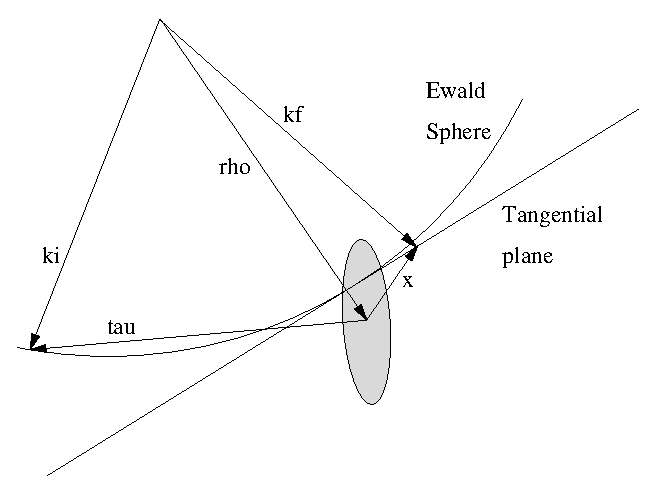
\includegraphics[width=0.7\textwidth]{figures/recip-detail.eps}
%  \end{center}
%\caption{The scattering triangle in the single crystal.}
%\label{fig:crystal-scattering-tri}
%\end{figure}
%
%The equation for the plane is
%\begin{equation}
%  \label{eq:crystal-tangent-plane}
%    \boldsymbol{P}(\boldsymbol{t}) = \boldsymbol{o} + B \boldsymbol{t}, \qquad
%    \boldsymbol{t} \in \mathbb{R}^2
%\end{equation}
%Here $B = (\boldsymbol{b}_1, \boldsymbol{b}_2)$ is a $3\times 2$ matrix
%with the two generators for the plane $\boldsymbol{b}_1$ and
%$\boldsymbol{b}_2$. These are (arbitrary) unit vectors in the plane,
%being perpendicular to
%each other and to the plane normal $\boldsymbol{n} =
%\boldsymbol{\rho}/\rho$.
%
%Each $\boldsymbol{t}$ defines a potential final wave vector
%$\boldsymbol{k}_{\rm f}(\boldsymbol{t}) = \boldsymbol{k}_{\rm i} +
%\boldsymbol{P}(\boldsymbol{t})$. The value of the 3-dimensional Gaussian
%for this $\boldsymbol{k}_{\rm f}$ is
%\begin{equation}
%  \label{eq:crystal-gauss-t-1}
%  G(\boldsymbol{x}(\boldsymbol{t})) =
%  \frac{1}{(\sqrt{2\pi})^3}\frac{1}{\sigma_1\sigma_2\sigma_3}
%  e^{-\boldsymbol{x}(\boldsymbol{t})^{\rm T} D \boldsymbol{x}(\boldsymbol{t})}
%\end{equation}
%where $\boldsymbol{x}(\boldsymbol{t}) = \boldsymbol{\tau} -
%(\boldsymbol{k}_{\rm i} - \boldsymbol{k}_{\rm f}(\boldsymbol{t}))$ is
%given in local coordinates for $\boldsymbol{\tau}$. It can be shown that
%equation~(\ref{eq:crystal-gauss-t-1}) can be re-written as
%\begin{equation}
%  \label{eq:crystal-gauss-2}
%  G(\boldsymbol{x}(\boldsymbol{t})) =
%  \frac{1}{(\sqrt{2\pi})^3}\frac{1}{\sigma_1\sigma_2\sigma_3} e^{-\alpha}
%  e^{-(\boldsymbol{t}-\boldsymbol{t}_0)^{\rm T} M
%    (\boldsymbol{t}-\boldsymbol{t}_0)}
%\end{equation}
%where $M = B^{\rm T} D B$ is a $2 \times 2$ symmetric and positive
%definite matrix, $\boldsymbol{t}_0 = -M^{-1}B^{\rm T} D \boldsymbol{o}$
%is a 2-vector, and $\alpha = -\boldsymbol{t}_0^{\rm T} M
%\boldsymbol{t}_0 + \boldsymbol{o}^{\rm T} D \boldsymbol{o}$ is a real
%number.  Note that this is a two-dimensional Gaussian (not necessarily
%normalized) in $\boldsymbol{t}$ with center $\boldsymbol{t}_0$ and axis
%defined by $M$.
%
%To choose $\boldsymbol{k}_{\rm f}$ we sample $\boldsymbol{t}$ from the
%2-dimensional Gaussian distribution~(\ref{eq:crystal-gauss-2}). To do
%this, we first construct the Cholesky decomposition of the matrix
%$(\frac{1}{2}M^{-1})$. This gives a $2\times 2$ matrix $L$ such that $L
%L^{\rm T} = \frac{1}{2}M^{-1}$ and is possible since $M$ is symmetric
%and positive definite. It is given by
%$$
%  L = \left(
%  \begin{array}[c]{cc}
%    \sqrt{\nu_{11}} & 0 \\
%    \frac{\nu_{12}}{\sqrt{\nu_{11}}} & \sqrt{\nu_{22} - \frac{\nu_{12}^2}{\nu_{11}}}
%  \end{array}\right)
%\qquad\hbox{where }
%  \frac{1}{2}M^{-1} = \left(
%  \begin{array}[c]{cc}
%    \nu_{11} & \nu_{12} \\
%    \nu_{12} & \nu_{22}
%  \end{array}\right)
%$$
%Now let $\boldsymbol{g} = (g_1, g_2)$ be two random numbers drawn form a
%Gaussian distribution with mean 0 and standard deviation 1, and let
%$\boldsymbol{t} = L\boldsymbol{g} + \boldsymbol{t}_0$. The probability
%of a particular $\boldsymbol{t}$ is then
%\begin{eqnarray}
%  P(\boldsymbol{t})d\boldsymbol{t}
%    &=& \frac{1}{2\pi}
%      e^{-\frac{1}{2}\boldsymbol{g}^{\rm T}\boldsymbol{g}} d\boldsymbol{g} \\
%    &=& \frac{1}{2\pi}\frac{1}{\det L}
%      e^{-\frac{1}{2}(L^{-1}(\boldsymbol{t}-\boldsymbol{t}_0))^{\rm T}
%          (L^{-1}(\boldsymbol{t}-\boldsymbol{t}_0))} d\boldsymbol{t} \\
%    &=& \frac{1}{2\pi}\frac{1}{\det L}
%      e^{-(\boldsymbol{t}-\boldsymbol{t}_0)^{\rm T}
%          M(\boldsymbol{t}-\boldsymbol{t}_0)} d\boldsymbol{t}
%  \label{eq:crystal-gauss-prob-1}
%\end{eqnarray}
%where we used that
%$\boldsymbol{g}=L^{-1}(\boldsymbol{t}-\boldsymbol{t}_0)$ so that
%$d\boldsymbol{g} = \frac{1}{\det L}d\boldsymbol{t}$. This is just the
%normalized form of~(\ref{eq:crystal-gauss-2}). Finally we set
%$\boldsymbol{k}'_{\rm f} = \boldsymbol{k}_{\rm i} +
%\boldsymbol{P}(\boldsymbol{t})$ and
%$\boldsymbol{k}_{\rm f} = (k_{\rm i}/k'_f)\boldsymbol{k}'_{\rm f}$ to
%normalize the length of $\boldsymbol{k}_{\rm f}$ to correct for the
%(small) error introduced by approximating the Ewald sphere with a plane.
%
%\subsection{Computing the total coherent cross-section}
%
%To determine the total coherent scattering cross-section, the differential
%cross-section must be integrated over the Ewald sphere:
%$$
%\sigma_{\rm coh} = \int_{\rm Ewald}
%\left(\frac{d\sigma}{d\Omega}\right)_{\rm coh.el.} d\Omega
%$$
%For small mosaic we may approximate the sphere with the tangential
%plane, and we thus get from~(\ref{eq:crystal-cross-section})
%and~(\ref{eq:crystal-gauss-2}):
%\begin{eqnarray}
%  \label{eq:crystal-coh-cs}
%  \sigma_{{\rm coh},\boldsymbol{\tau}} &=& \int N\frac{(2\pi)^3}{V_0}
%        G(\boldsymbol{\tau} - \boldsymbol{\kappa})
%         |F_{\boldsymbol{\tau}}|^2 d\Omega \\
%  &=& \frac{1}{\boldsymbol{k}_i^2} N\frac{(2\pi)^3}{V_0}
%         \frac{1}{(\sqrt{2\pi})^3}\frac{e^{-\alpha}}{\sigma_1\sigma_2\sigma_3}
%         |F_{\boldsymbol{\tau}}|^2
%         \int e^{-(\boldsymbol{t}-\boldsymbol{t}_0)^{\rm T} M
%         (\boldsymbol{t}-\boldsymbol{t}_0)}
%         d\boldsymbol{t} \\
%  &=& \det(L) \frac{1}{\boldsymbol{k}_i^2} N\frac{(2\pi)^{3/2}}{V_0}
%         \frac{e^{-\alpha}}{\sigma_1\sigma_2\sigma_3}
%         |F_{\boldsymbol{\tau}}|^2
%         \int e^{-\frac{1}{2}\boldsymbol{g}^{\rm T}\boldsymbol{g}}
%         d\boldsymbol{g} \\
%  &=& 2\pi\det(L) \frac{1}{\boldsymbol{k}_i^2} N\frac{(2\pi)^{3/2}}{V_0}
%         \frac{e^{-\alpha}}{\sigma_1\sigma_2\sigma_3}
%         |F_{\boldsymbol{\tau}}|^2 \\
%  &=& \frac{\det(L)}{\boldsymbol{k}_i^2} N\frac{(2\pi)^{5/2}}{V_0}
%         \frac{e^{-\alpha}}{\sigma_1\sigma_2\sigma_3}
%         |F_{\boldsymbol{\tau}}|^2 \\
%  \sigma_{\rm coh} &=& \sum_{\boldsymbol{\tau}} \sigma_{{\rm coh},\boldsymbol{\tau}}
%\end{eqnarray}
%As before, we let $\boldsymbol{g} = L^{-1}(\boldsymbol{t} -
%\boldsymbol{t}_0)$ so that $d\boldsymbol{t} = \det(L) d\boldsymbol{g}$.
%
%\paragraph{Neutron weight factor adjustment}
%
%We now calculate the correct neutron weight adjustment for the Monte
%Carlo choices made. In three cases is a Monte Carlo choice made with a
%probability different from the probability of the corresponding physical
%event: When deciding whether to transmit the neutron or not, when
%simulating absorption, and when selecting the reciprocal lattice vector
%$\boldsymbol{\tau}$ to scatter from.
%
%If the user has choosen a fixed transmission probability $f({\rm
%  transmit}) = p_{\rm transmit}$, the neutron weight must be adjusted by
%$$ \pi({\rm transmit}) = \frac{P({\rm transmit})}{f({\rm transmit})}
%$$
%where $P({\rm transmit}) = \exp(-\frac{\sigma_{\rm tot}}{V_0}\ell)$ is
%the physical transmission probability. Likewise, for non-transmission
%the adjustment is
%$$ \pi({\rm no~transmission}) = \frac{1-P({\rm transmit})}{1-f({\rm transmit})}.
%$$
%
%Absorption is never explicitly simulated, so the Monte Carlo probability
%of coherent or incoherent scattering is
%$f({\rm coh})+f({\rm inc}) = 1$.
%The physical probability of coherent or incoherent scattering is
%$$ P({\rm coh})+P({\rm inc}) = \frac{\sigma_{\rm coh} + \sigma_{\rm
%    inc}}{\sigma_{\rm tot}}, $$
%so again a weight adjustment $\pi({\rm coh}|{\rm inc}) = \Pi({\rm
%    coh}|{\rm inc})/f({\rm coh}|{\rm inc})$ is needed.
%
%When choosing the reciprocal lattice vector $\boldsymbol{\tau}$ to
%scatter from, the relative probability for $\boldsymbol{\tau}$ is
%$r_{\boldsymbol{\tau}} = \sigma_{{\rm
%    coh},\boldsymbol{\tau}}/|F_{\boldsymbol{\tau}}|^2$. This is done to
%get better statistics for weak reflections. The Monte Carlo probability
%for the reciprocal lattice vector $\boldsymbol{\tau}$ is thus
%$$ f(\boldsymbol{\tau}) =
%\frac{r_{\boldsymbol{\tau}}}{\sum_{\boldsymbol{\tau}} r_{\boldsymbol{\tau}}}
%$$
%whereas the physical probability is $P(\boldsymbol{\tau}) = \sigma_{{\rm
%    coh},\boldsymbol{\tau}}/\sigma_{\rm coh}$. A weight adjustment is
%thus needed of
%$$
%\pi(\boldsymbol{\tau}) =
% \frac{P(\boldsymbol{\tau})}{f(\boldsymbol{\tau})} =
% \frac{\sigma_{{\rm coh},\boldsymbol{\tau}}
%  \sum_{\boldsymbol{\tau}} r_{\boldsymbol{\tau}}}
% {\sigma_{\rm coh} \; r_{\boldsymbol{\tau}}}.$$
%
%In most cases, however, only one reflection is possible, whence $\pi=1$.
%
%\subsection{Implementation details}
%\label{s:Single_crystal_implement}
%
%The equations describing {\bf Single\_crystal} are quite
%complex, and consequently the code is fairly sizeable. Most of it is
%just the expansion of the vector and matrix equations in individual
%coordinates, and should thus be straightforward to follow.
%
%The implementation pre-computes a lot of the necessary values in the
%\texttt{INITIALIZE} section. It is thus actually very efficient despite
%the complexity. If the list of reciprocal lattice points is big,
%however, the search through the list will be slow. The precomputed data
%is stored in the structures \texttt{hkl\_info} and in an array of
%\texttt{hkl\_data} structures (one for each reciprocal lattice point in
%the list). In addition, for every neutron event an array of
%\texttt{tau\_data} is computed with one element for each reciprocal
%lattice point close to the Ewald sphere. Except for the search for
%possible $\boldsymbol{\tau}$ vectors, all computations are done in local
%coordinates using the matrix $U$ to do the necessary transformations.
%
%The list of reciprocal lattice points is specified in an ASCII data
%file. Each line contains seven numbers, separated by white space. The
%first three numbers are the $(h,k,l)$ indices of the reciprocal lattice
%point, and the last number is the value of the structure factor
%$|F_{\boldsymbol{\tau}}|^2$, in barns. The middle three numbers are not
%used and may be omitted; they are nevertheless recommended since this makes
%the file format compatible with the output from the Crystallographica
%program~\cite{crystallographica}.
%Any line beginning with any character of \verb+#;/%+ is considered to be a
%comment, and lines which can not be read as vectors/matrices are ignored.
%
%The column signification may also explicitely be set in the data file header using any of the lines:
%\begin{verbatim}
%  #column_h <index of the Bragg Qh column>
%  #column_k <index of the Bragg Qk column>
%  #column_l <index of the Bragg Ql column>
%  #column_F2 <index of the squared str. factor '|F|^2' column [b]>
%  #column_F  <index of the structure factor norm '|F|' column>
%\end{verbatim}
%
%Other component parameters may as well be specified in the data file
%header with lines e.g.:
%\begin{verbatim}
%  #sigma_abs <value of Absorption cross section [barns]>
%  #sigma_inc <value of Incoherent cross section [barns]>
%  #Delta_d/d <value of Detla_d/d width for all lines>
%  #lattice_a <value of the a lattice parameter [Angs]>
%  #lattice_a <value of the b lattice parameter [Angs]>
%  #lattice_a <value of the c lattice parameter [Angs]>
%  #lattice_aa <value of the alpha lattice angle [deg]>
%  #lattice_bb <value of the beta  lattice angle [deg]>
%  #lattice_cc <value of the gamma lattice angle [deg]>
%\end{verbatim}
%
%Example data \verb+*.lau+ files are given in directory \verb+MCXTAS/data+.
%
%These files contain an extensive self-documented header defining most the sample parameters, so that only the file name and mosaicity should be given to the component:
%\begin{verbatim}
%  Single_crystal(xwidth=0.01, yheight=0.01, zdepth=0.01,
%    mosaic = 5, reflections="YBaCuO.lau")
%\end{verbatim}
%
%Powder files from ICSD/LAZY \cite{icsd_ill} and Fullprof \cite{Fullprof}
%may also be used (see Table \ref{t:powders-data}, page \pageref{t:powders-data}).
%We do not recommend to use these as the equivalent $\vec q$ vectors are superposed, not
%all Bragg spots will be simulated, and the intensity will not be scaled by the
%multiplicity for each spot.
%
   \newpage
\section{Molecule\_2state: Excitable time-dependent sample model}
\index{Samples!liquid, diffraction}
\index{DFT}
\index{time resolved}
\label{molecule_2state}

\mcdoccomp{samples/Molecule_2state.parms}

Further Documentaion pending
 \newpage
%\input{samples/saxs.tex}             \newpage
%\input{samples/absorption_phantom.tex} \newpage
%\section{Phonon\_simple: A simple phonon sample}
\label{s:phonon_simple}
\index{Samples!Phonon scattering}
\index{Inelastic scattering}

\component{Phonon\_simple}{Kim Lefmann, Ris\o\ National Laboratory}{ $r_{\rm o}$, $h$, $r_{\rm foc}$, $x_{\rm target}$, $y_{\rm target}$, $z_{\rm target}$, $\sigma_{\rm abs}$, $\sigma_{\rm inc}$, $a$, $b$, $c$, $M$, $DW$, $T$}{$w_x$, $h_y$, $t_z$, $w_{\rm focus}, h_{\rm focus}$, $w_{\rm foc, angle}$, $h_{\rm foc, angle}$, target\_index}{only validated qualitatively}

This component models a simple phonon signal from a single crystal of
a pure element in an {\em fcc} crystal structure.
Only one isotropic acoustic phonon branch is modelled, and the longitudinal
and transverse dispersions are identical with the velocity of sound being $c$.
Other physical parameters are the atomic mass, $M$, the lattice parameter, $a$,
the scattering length, $b$,
the Debye-Waller factor, \verb+DW+, and the temperature, $T$.
Incoherent scattering and absorption are taken into account by the cross
sections $\sigma_{\rm abs}$ and $\sigma_{\rm inc}$.

The sample can have the form of a cylinder with height $h$ and radius
$r_0$, or a box with dimensions $w_x, h_y, t_z$.

Phonons are emitted into a specific range of solid angles, specified
by the location $(x_t, y_t, z_t)$ and the focusing radius, $r_0$.
Alternatively, the focusing is given by a rectangle,
$w_{\rm focus}$ and $h_{\rm focus}$, and the focus point is given by the
index of a down-stream component, \verb+target_index+.

Multiple scattering is not included in this component.

A usage example of this component can be found in the \verb+Neutron site/tests/Test_Phonon+ instrument from the \verb+mcgui+.

\subsection{The phonon cross section} % This is modified from the paper version %
The inelastic phonon cross section for a Bravais crystal of a pure element
is given by Ref.~\cite[ch.3~]{squires}
\begin{eqnarray}
\frac{d^2\sigma'}{d\Omega dE_{\rm f}} &=&
  b^2 \frac{k_{\rm f}}{k_{\rm i}} \frac{(2\pi)^3}{V_0}\frac{1}{2M} \exp(-2W) \nonumber \\
&\times&
  \sum_{\tau,q,p} \frac{(\mbox{\boldmath $\kappa$} \cdot {\bf e}_{q,p})^2}
                       {\omega_{q,p}}
  \left\langle n_{q,p} + \frac{1}{2} \mp \frac{1}{2} \right\rangle
  \delta(\omega\pm\omega_{q,p}) \delta(\kappa\pm{\bf q}-\tau) ,
\end{eqnarray}
where both annihilation and creation of one phonon is considered
(represented by the plus and minus sign in the dispersion delta functions,
respectively).
In the equation,
$\exp(-2W)$ is the Debye-Waller factor, \verb+DW+ and
$V_0 $ is the volume of the unit cell.
The sum runs over the reciprocal lattice vectors, $\tau$,
over the polarisation index, $p$,
and the $N$ allowed wave vectors {\bf q} within the Brillouin zone
(where $N$ is the number of unit cells in the crystal).
Further, ${\bf e}_{q,p}$ is the
polarization unit vectors, $\omega_{q,p}$ the phonon dispersion,
and the Bose factor is
$\langle n_{q,p} \rangle = (\hbar \exp(|\omega_{q,p}|/k_{\rm B}T)-1)^{-1}$.

We have simplified this expression by assuming no polarization
dependence of the dispersion, giving
$\sum_{p} (\mbox{\boldmath $\kappa$} \cdot {\bf e}_{q,p})^2 = \kappa^2$.
We assume that the inter-atomic interaction is nearest-neighbour-only
so that the phonon dispersion becomes:
\begin{equation}
d_1({\bf q}) = c_1/a \sqrt{z-s_q} ,
\end{equation}
where $z=12$ is the number of nearest neighbours and
$s_q=\sum_{\rm nn} \cos({\bf q} \cdot {\bf r}_{\rm nn})$,
where in turn ${\bf r}_{\rm nn}$ is the lattice positions of the
nearest neighbours.

This dispersion relation may be modified with a small effort,
since it is given as a separate c-function attatched to the component.

To calculate $d\sigma/d\Omega$ we need to transform the
{\bf q} sum into an integral over the Brillouin zone by
$\sum_q \rightarrow N V_{\rm c} (2\pi)^{-3} \int_{\rm BZ} d^3{\bf q}$.
The $\mbox{\boldmath $\kappa$}$ sum can now be removed by
expanding the {\bf q} integral to infinity.
All in all, the partial differential cross section reads
\begin{eqnarray}
\frac{d^2\sigma'}{d\Omega dE_{\rm f}}
  (\mbox{\boldmath $\kappa$},\omega) &=&
  N b^2 \frac{k_{\rm f}}{k_{\rm i}} \frac{1}{2M}
  \int \frac{\hbar \kappa^2}{\hbar \omega_q}
  \left\langle n_{q}+\frac{1}{2}\mp\frac{1}{2} \right\rangle
  \delta(\omega\pm\omega_{q}) \delta(\mbox{\boldmath $\kappa$}\pm{\bf q})
   d^3{\bf q} \nonumber \\
 &=& N b^2 \frac{k_{\rm f}}{k_{\rm i}}
          \frac{\hbar^2 \kappa^2}{2M \hbar \omega_q}
  \left\langle n_{\kappa}+\frac12\pm\frac12 \right\rangle
  \delta(\hbar\omega\pm d_1(\kappa)) . \label{e:phonon-pdcross}
\end{eqnarray}

\subsection{The algorithm}
All neutrons, which hit the sample volume, are scattered
into a particular range of solid angle, $\Delta \Omega$,
like many other components. One of the difficult things in
scattering from a dispersion is to take care to fulfill the
dispersion criteria and to find the correct weight transformation.

In {\bf Phonon\_simple}, the following steps are taken:
\begin{enumerate}
\item If the sample is hit, calculate the total path length inside the
sample, otherwise leave the neutron ray unchanged.
\item Choose a scattering point inside the sample
\item Choose a direction for the final wave vector, $\hat{\bf k}_{\rm f}$
within $\Delta\Omega$.
\item Calculate possible values of $k_{\rm f}$ so that the
dispersion relation is fulfilled for the corresponding value
of ${\bf k}_{\rm f}$. (There is always at least one possible $k_{\rm f}$
value \cite{bacon}.)
\item Choose one of the calculated $k_{\rm f}$ values.
\item Propagate the neutron to the scattering point and adjust the
neutron velocity according to $k_{\rm f}$.
\item Calculate and apply the correct weight factor correction, see below.
\end{enumerate}

\subsection{The weight transformation}
Before making the weight transformation, we need to calculate the
probability for scattering along one certain direction $\Omega$
from one phonon mode. To do this, we must integrate out the delta
functions in the cross section (\ref{e:phonon-pdcross}).
We here use that $\hbar \omega_q = \hbar^2 (k_i^2 - k_f^2) / (2 m_{\rm N})$,
$\kappa = {\bf k}_{\rm i} - k_{\rm f}\hat{\bf k}_f$, and
the integration rule $\int \delta(f(x)) = (df/dx)(0)^{-1}$.
Now, we reach
\begin{equation} \label{eq:phononcross}
\left(\frac{d\sigma'}{d\Omega}\right)_j = \int \frac{d^2\sigma'}{d\Omega dE_{\rm f}} dE_{\rm f}
 = N b^2 \frac{k_{\rm f}}{k_{\rm i}}
\frac{\hbar^2 \kappa^2}{2M d_1(\kappa_j) J(k_{{\rm f},j})}
\left\langle n_{\kappa}+\frac12\pm\frac12 \right\rangle .
\end{equation}

where the Jacobian reads
\begin{equation}
J = 1 - \frac{m_{\rm N}}{k_{\rm f} \hbar^2}
    \frac{\partial}{\partial k_{\rm f}} \left( d_1(\kappa) \right) .
\end{equation}

A rough order-of-magnitude consideration gives
$\frac{k_{{\rm f},j}}{k_{\rm i}}\approx 1$,
$J \approx 1$,
$\langle n_{\kappa}+\frac12\pm\frac12 \rangle \approx 1$,
$\frac{\hbar^2\kappa^2}{2M d_1(\kappa)}
\approx \frac{m}{M}$.
Hence, $\left(\frac{d\sigma}{d\Omega}\right)_j \approx N b^2 \frac{m}{M}$, and
the phonon cross section becomes a fraction of
the total scattering cross section $4 \pi N b^2$, as it must be.
The differential cross section per unit volume is found from
(\ref{eq:phononcross}) by replacing $N$ with $1/V_0$.

The total weight transformation now becomes
\begin{equation} \label{eq:phonon_mult}
\pi_i = a_{\rm lin} l_{\rm max} n_{\rm s} \Delta \Omega
 b^2 \frac{k_{{\rm f},j}}{k_{\rm i}}
 \frac{\hbar^2 \kappa}{2 V_0 M d_1(\kappa) J(k_{{\rm f},j})}
 \left\langle n_{\kappa}+\frac12 \pm\frac12 \right\rangle ,
\end{equation}
where $n_s$ is the number of possible dispersion values in the chosen direction.

The \verb+Test_Phonon+ test/example instrument exists in the distribution for this component.
           \newpage
%\input{LSCO.tex}            \newpage
%\section{Isotropic\_Sqw: A general $S(q,\omega)$ coherent and incoherent scatterer}
\label{s:isotropic-sqw}
\index{Samples!Coherent and incoherent isotropic scatterer}
\index{Coherent and incoherent isotropic scatterer}
\index{Inelastic scattering}
\index{Sample environments}
\index{Concentric components}
\index{Multiple scattering}

\component{Isotropic\_Sqw}{V. Hugouvieux, E. Farhi}{Sqw$\_{coh}$, $\sigma_{coh}$, Sqw$\_{inc}$, $\sigma_{inc}, V_\rho, \sigma_{abs}, T$,$x_{width},y_{height},z_{depth},r$, thickness}{$q_{min}, q_{max}, \omega_{min}, \omega_{max}, d\phi$, order}{validated (Vanadium, l-Rb, PowderN more accurate for powders) }

\begin{figure}
  \begin{center}
    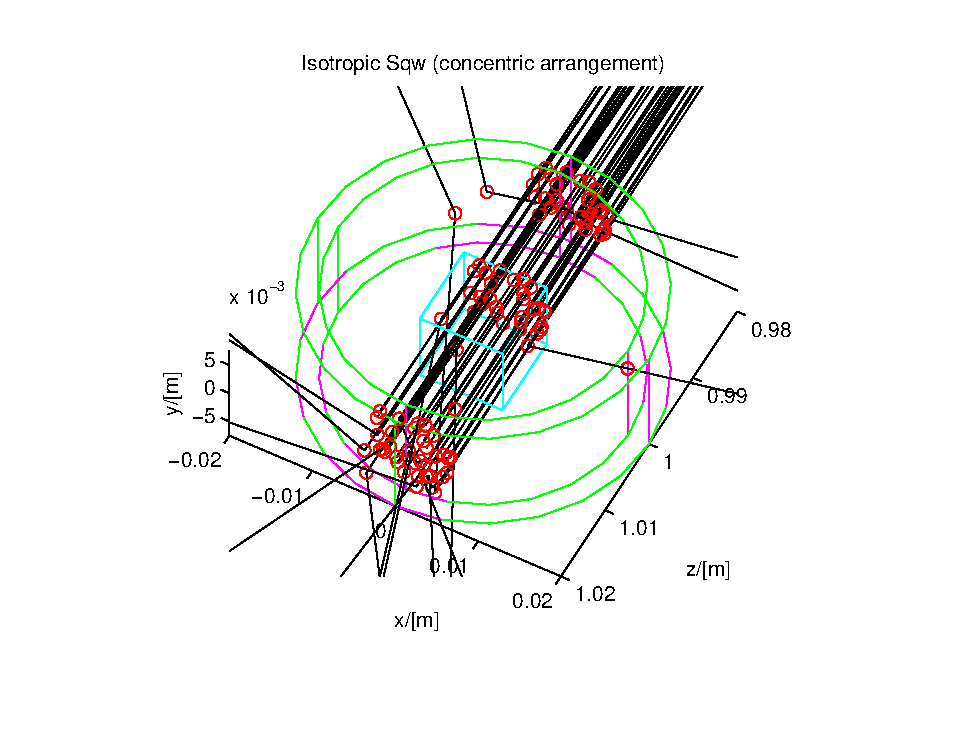
\includegraphics[width=0.9\textwidth]{figures/sqw}
  \end{center}
\caption{An $l-^4$He sample in a cryostat, simulated with the Isotropic\_Sqw component in concentric geometry.}
\label{f:isotropic-sqw}
\end{figure}

The sample component \emph{Isotropic\_Sqw} has been developed in order to simulate neutron scattering from any isotropic material such as liquids, glasses (amorphous systems), polymers and powders (currently, mono-crystals cannot be handled).
The component treats coherent and incoherent neutron scattering and may be used to model most materials, including sample environments with concentric geometries.
The structure and dynamics of isotropic samples can be characterised by the dynamic structure factor $S(q,\omega)$, which determines the interaction between neutrons and the sample and therefore can be used as a probability distribution of $\omega$-energy and $q$-momentum transfers. It handles coherent and incoherent processes, both for elastic and inelastic interactions.
The main input for the component is $S(q,\omega)$ tables, or powder structure files.

Usage examples of this component can be found in the \\
\verb+Neutron site/tests/Test_Isotropic_Sqw+, the \\
\verb+Neutron site/ILL/ILL_H15_IN6+ and the \verb+ILL_TOF_Env+ instruments from the \verb+mcgui+.

\subsection{Neutron interaction with matter - overview}

When a neutron enters a material, according to usual models, it 'sees' atoms as disks with a surface equal to the total cross section of the material $\sigma_{tot}$. The latter includes absorption, coherent and incoherent contributions, which all depend on the incoming neutron energy.
The transmission probability follows an exponential decay law accounting for the total cross section.

For the neutron which is not transmitted, we select a scattering position along the path, taking into account the secondary extinction and absorption probability. In this process, the neutron is considered to be a particle or an attenuated wave.

Once a scattering position has been assigned, the neutron interacts with a material excitation. Here we turn to the wave description of the neutron, which interacts with the whole sample volume. The distribution of excitations, which determines their relative intensity in the scattered beam, is simply the dynamic structure factor - or scattering law - $S(q,\omega)$. We shall build probability distributions from the scattering law in order to improve the efficiency of the method by favoring the $(q,\omega)$ choice towards high $S(q,\omega)$ regions.

The neutron leaves the scattering point when a suitable $(q, \omega)$ choice has been found to satisfy the conservation laws. The method is iterated until the neutron leaves the volume of the material, therefore allowing multiple scattering contributions, which will be considered in more details below.

No experimental method makes it possible to accurately measure the multiple scattering contribution, even though it can become significant at low $q$ transfers (below the first diffraction maximum), where the single scattering coherent signal is weak in most materials. This is why attemps have been made to reduce the multiple scattering contribution by partitioning the sample with absorbing layers. However, this is not always applicable thus makiong the simulation approach very valuable.

The method presented here for handling neutron interaction with isotropic materials is similar in many respects to the earlier MSC \cite{msc}, Discus \cite{discus} and MSCAT \cite{mscat} methods, but the implementation presented here is part of a more general treatment of a sample in an instrument.

\subsection{Theoretical side}

\subsubsection{Pair correlation function $g(r)$ and Dynamic structure factor $S(q,\omega)$}

In the following, we consider an isotropic medium irradiated with a cold or thermal neutron beam. We ignore the possible thermal fission events and assume that the incoming neutron energy does not correspond to a Breit-Wigner resonance in the material. Furthermore, we do not take into account quantum effects in the material, nor refraction and primary extinction.

Following Squires \cite{squires}, the experimental counterpart of the scattering law $S(q,\omega)$ is the neutron double differential scattering cross section for both coherent and incoherent processes:
\begin{equation}\label{eq:d2sigma}
\frac{d^2\sigma}{d\Omega dE_f} = \frac{\sigma}{4\pi}\frac{k_f}{k_i} N S(q, \omega)
\end{equation}
which describes the amount of neutrons scattered per unit solid angle $d\Omega$ and per unit final energy $dE_f$. In this equation, $N=\rho V$ is the number of atoms in the scattering volume $V$ with atomic number density $\rho$, $E_f, E_i, k_f, k_i$ are the kinetic energy and wavevectors of final and initial states respectively, $\sigma$ is the bound atom scattering cross-section, $\Omega$ is the solid angle and $q,\omega$ are the wave-vector and energy transfer at the sample. In practice, the double differential cross section is a linear combinaison of the coherent and incoherent parts as:
\begin{equation}
\label{eq:S=coh+inc}
\sigma S(q,\omega) = \sigma_{coh} S_{coh}(q,\omega) + \sigma_{inc} S_{inc}(q,\omega)
\end{equation}
where the subscripts $coh$ and $inc$ stand for the coherent and incoherent contributions respectively.

We define its norm on a selected $q$ range:
\begin{equation}
|S| = \iint S(q,\omega) dq d\omega .
\end{equation}
The norm $\lim_{q \rightarrow \infty} |S| \simeq q$ for large $q$ values, and can only be defined on a restricted $q$ range.

Some easily measureable coherent quantities in a liquid are the \emph{static pair correlation function} $g(r)$ and the \emph{structure factor} $S(q)$, defined as:
\begin{eqnarray}
\rho g(\vec{r}) &=& \frac{1}{N} \sum_{i=1}^N \sum_{j \neq i} \langle \delta(\vec{r}+\vec{r}_i-\vec{r}_j) \rangle \\
S(\vec{q}) &=&\int S(\vec q,\omega) d\omega \label{eq:sq} \\
           &=&1 + \rho \int_V [g(\vec{r})-1] e^{i\vec{q}.\vec{r}} d\vec{r} \\
           &=&1 + \rho \int_{0}^{\infty} [g(r)-1] \frac{\sin(qr)}{qr} 4 \pi r^2 dr {\rm\ in\ isotropic\ materials.}
\end{eqnarray}
The latter expression, in isotropic materials, may be Fourier transformed as:
\begin{equation}
\label{eq:gr-sq}
g(r)-1 =\frac{1}{2\pi^2 \rho} \int_0^\infty q^2 [S(q) -1] \frac{sin(qr)}{qr} dq
\end{equation}
Both $g(r)$ and $S(q)$ converge to unity for large $r$ and $q$ values respectively, and they are representative of the atoms spatial distribution. In a liquid $\lim_{q \rightarrow 0} S(q) = \rho k_B T \chi_T$ where $\chi_T=(\frac{\partial \rho}{\partial P})_{V,T}$ is the compressibility \cite{Egelstaff67,fischer05}. In perfect gases, $S(q) = 1$ for all $q$. These quantities are obtained experimentally from diffractometers.
In principle, $S_{inc}(q) = 1$ in all materials, but a $q$ dependence is rather usual, partly due to the Debye-Waller factor $e^{-q^2 \langle u^2 \rangle}$. Anyway, $S_{inc}(q)$ converges to unity at high $q$.

The static pair correlation function $g(r)$ is the probability to find a neighbouring atom at a given distance (unitless). Since $g(0) = 0$, Eq. (\ref{eq:gr-sq}) provides a useful normalisation sum-rule for coherent $S(q)$:
\begin{equation}
\label{eq:sq-nomr1}
\int_0^\infty q^2 [S(q) - 1] dq = -2\pi^2\rho {\rm\ for\ coherent\ contribution.}
\end{equation}
This means that the integrated oscillations (around 1) of $S_{coh}(q)$ are directly related to the density of the material $\rho$.
In practice, the function $S(q)$ is often known on a restricted range $q \in [0, q_{max} ]$, due to either limitations in the sample molecular dynamics simulation, or the measurement itself.
In first approximation we consider that Eq. (\ref{eq:sq-nomr1}) can be applied in this range, i.e. we neglect the large $q$ contributions provided $S(q)-1$ converges faster than $1/q^2$. This is usually true after 2-3 oscillations of $S(q)$ in liquids.
Then, in isotropic liquid-like materials, Eq. (\ref{eq:sq-nomr1}) provides a normalisation sum-rule for $S$.

\subsection{Theoretical side - scattering in the sample}

The Eq. \ref{eq:d2sigma} controls the scattering in the whole sample volume.
Its implementation in a propagative Monte Carlo neutron code such as \emph{McStas} can be summarised as follows:
\begin{enumerate}
{\item Compute the propagation path length in the material by geometrical intersections between the neutron trajectory and the sample volume.}
{\item Evaluate the total cross section from the integration of the scattering law over the accessible dynamical range (Section \ref{s:inter-proba}).}
{\item Use the total cross section to determine the probability of interaction for each neutron along the path length, and select a scattering position.}
{\item Weight neutron interaction with the absorption probability and select the type of interaction (coherent or incoherent).}
{\item Select the wave vector and energy transfer from the dynamic structure factor $S(q,\omega)$ used as a probability distribution (Section \ref{s:choose-qw}). Apply the detailed balance.}
{\item Check whether selection rules can be solved (Section \ref{s:rules-qw}). If they cannot, repeat (5).}
\end{enumerate}
This procedure is iterated until the neutron leaves the sample. We shall now detail the key steps of this implementation.

\subsubsection{Evaluating the cross sections and interaction probability}
\label{s:inter-proba}

Following Sears \cite{Sears75}, the total scattering cross section for incoming neutrons with initial energy $E_i$ is
\begin{equation}
\label{eq:iisigma}
\sigma_s(E_i) = \iint \frac{d^2 \sigma}{d\Omega dE_f} d\Omega dE_f = \frac{N \sigma}{4\pi} \iint \frac{k_f}{k_i} S(q, \omega) d\Omega dE_f
\end{equation}
where the integration runs over the entire space and all final neutron energies.
As the dynamic structure factor is defined in the $q,\omega$ space, the integration requires a variable change. Using the momentum conservation law and the solid angle relation $\Omega=2\pi(1-cos \theta)$, were $\theta$ is the solid angle opening, we draw:
\begin{equation}
\label{eq:iqSqw}
\sigma_s(E_i) = N \iint \frac{\sigma S(q,\omega) q}{2 k_i^2} dq d\omega.
\end{equation}
This integration runs over the whole accessible $q,\omega$ dynamical range for each incoming neutron.
In practice, the knowledge of the dynamic structure factor is defined over a limited area with $q \in [q_{min}, q_{max}]$ and $\omega \in [\omega_{min}, \omega_{max}]$ which is constrained by the method for obtaining $S(q,\omega)$, i.e. from previous experiments, molecular dynamics simulations, and analytical models. It is desirable that this area be as large as possible, starting from 0 for both ranges. If we use $\omega_{min} \rightarrow 0$, $q_{min} \rightarrow 0$, $\omega_{max} > 4E_i$ and $q_{max} > 2k_i$, we completely describe all scattering processes for incoming neutrons with wavevector $k_i$ \cite{msc}.

This means that in order to correctly estimate the total intensity and multiple scattering, the knowledge of $S(q,\omega)$ must be wider (at least twice in $q$, as stated previously) than the measurable range in the corresponding experiment.
As a side effect, a self consistent iterative method for finding the true scattering law from the measurement itself is not theorically feasible, except for providing crude approximations.
However, that measured dynamic structure factor may be used to estimate the multiple scattering for a further measurement using longer wavelength neutrons.
In that case, extrapolating the scattering law beyond the accessible measurement ranges might improve substantially the accuracy of the method, but this discussion is beyond the scope of this paper.

Consequently, limiting the $q$ integration in Eq. \ref{eq:iqSqw} to the maximum momentum transfer for elastic processes $2 k_i$, we write the total scattering cross section as
\begin{equation}
\label{eq:iqSq}
\sigma_s(E_i) \simeq \frac{N}{2 k_i^2} \int_0^{2k_i} q \sigma S(q) dq.
\end{equation}
Using Eq. \ref{eq:S=coh+inc}, it is possible to define similar expressions for the coherent and incoherent terms $\sigma_{coh}(E_i)$ and $\sigma_{inc}(E_i)$ respectively. These integrated cross sections are usually quite different from the tabulated values \cite{ILLblue} since the latter are bound scattering cross sections.

Except for a few materials with absorption resonances in the cold-thermal energy range, the absorption cross section for an incoming neutron of velocity $v_i=\sqrt{2E_i/m}$, where $m$ is the neutron mass, is computed as
$\sigma_{abs}(E_i) = \sigma_{abs}^{{\rm 2200}}\frac{2200 m/s}{\sqrt{2E_i/m}}$, where $\sigma_{abs}^{{\rm 2200}}$ is obtained from the literature \cite{ILLblue}.

We now determine the total cross section accounting for both scattering and absorption
\begin{equation}
\sigma_{tot}(E_i) = \sigma_{abs}(E_i) + \sigma_s(Ei).
\end{equation}
The neutron trajectory intersection with the sample geometry provides the total path length in the sample $d_{exit}$ to the exit.
Defining the linear attenuation $\mu(E_i) = \rho\sigma_{tot}(E_i)$, the probability that the neutron event is transmitted along path $d_{exit}$ is $e^{-\mu(E_i) d_{exit}}$.

If the neutron event is transmitted, it leaves the sample. In previous Monte Carlo codes such as DISCUSS \cite{discus}, MSC \cite{msc} and MSCAT \cite{mscat}, each neutron event is forced to scatter to the detector area in order to improve the sample scattering simulation statistics and reduce the computing time. The corresponding instrument model is limited to a neutron event source, a sample and a detector. It is equaly possible in the current implementation to 'force' neutron events to scatter by applying a correction factor $\pi_0=1-e^{-\mu(E_i) d_{exit}}$ to the neutron statistical weight. However, the \emph{McStas} instrument model is often build from a large sequence of components. Eventhough the instrument description starts as well with a neutron event source, more than one sample may be encountered in the course of the neutron propagation and multiple detectors may be positioned anywhere in space, as well as other instrument components (e.g. neutron optics). This implies that neutron events scattered from a sample volume should not focus to a single area.  Indeed, transmitted events may reach other scattering materials and it is not desirable to force all neutron events to scatter. The correction factor $\pi_0$ is then not applied, and neutron events can be transmitted through the sample volume. The simulation efficiency for the scattering then drops significantly, but enables to model much more complex arrangements such as concentric sample environments, magnets and monochromator mechanical parts, and neutron filters.

If the neutron is not transmitted, the neutron statistical weight is multiplied by a factor
\begin{equation}
\pi_1 = \frac{\sigma_s(E_i)}{\sigma_{tot}(E_i)}
\end{equation}
to account for the fraction of absorbed neutrons along the path, and we may in the following treat the event as a scattering event.
Additionally, the type of interaction (coherent or incoherent) is chosen randomly with fractions $\sigma_{coh}(E_i)$ and $\sigma_{inc}(E_i)$.

The position of the neutron scattering event along the neutron trajectory length $d_{exit}$ is determined by \cite{Mildner77,discus}
\begin{equation}
d_{s} = -\frac{1}{\mu(E_i)} \ln(1 - \xi[1 -e^{-\mu(E_i) d_{exit}}])
\end{equation}
where $\xi$ is a random number in [0,1]. This expression takes into account secondary extinction, originating from the decrease of the beam intensity through the sample (self shielding).

\subsubsection{Choosing the $q$ and $\omega$ transfer from $S(q, \omega)$ }
\label{s:choose-qw}

The choice of the $(q, \omega)$ wavevector-energy transfer pair could be done randomly, as in the first event of the second order scattering evaluation in DISCUS \cite{discus}, but it is somewhat inefficient except for materials showing a broad quasi-elastic signal. As the scattering originates from structural peaks and excitations in the material $S(q, \omega)$, it is usual \cite{mscat} to adopt an importance sampling scheme by focusing the $(q, \omega)$ choice to areas where the intensity of $S(q, \omega)$ is high. In practice, this means that the neutron event should scatter preferably on e.g. Bragg peaks, quasielastic contribution and phonons.

The main idea to implement the scattering from $S(q, \omega)$ is to cast two consecutive Monte Carlo choices, using probability distribution built from the dynamic structure factor.
We define first the probability $P_{\omega}(\omega)$ as the \emph{unweighted} fraction of modes whose energy lies between $\omega$ and $\omega+d\omega$
\begin{equation}
P_{\omega}(\omega) d\omega = \frac{\int_0^{q_{max}} q S(q,\omega) dq}{|S|},
\end{equation}
where $|S| = \iint S(q,\omega) dq d\omega$ is the norm of $S(q,\omega)$ in the available dynamical range $q \in [q_{min}, q_{max}]$ and $\omega \in [\omega_{min}, \omega_{max}]$.
The probability $P_{\omega}(\omega)$ is normalised to unity, $\int P_{\omega}(\omega) d\omega = 1$, and is a probability distribution of mode energies in the material. We then choose randomly an energy transfer $\omega$ from this distribution.

Similarly, in order to focus the wavevector transfer choice, we define the probability distribution of wavevector $P_q(q\mid\omega)$ for the selected energy transfer lying between $\omega$ and $\omega+d\omega$
\begin{equation}
P_q(q\mid\omega) = \frac{q S(q, \omega)}{S(q)},
\end{equation}
from which we choose randomly a wavevector transfer $q$, knowing the energy transfer $\omega$.
These two probability distributions extracted from $S(q,\omega)$ are shown in Fig. \ref{f:isotropic-sqw-proba}, for a model $S(q,\omega)$ function built from the {\it l}-$^4$He elementary excitation (Data from Donnelly).

\begin{figure}
  \begin{center}
    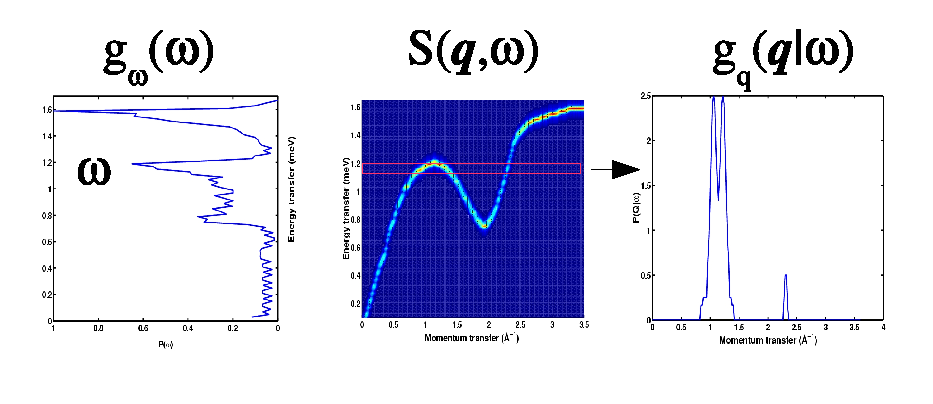
\includegraphics[width=0.9\textwidth]{figures/Sqw_sampling}
  \end{center}
\caption{\emph{Centre}: Model of dynamic structure factor $S(q,\omega)$ for l-$^4$He ; \emph{left}: probability distribution $g_\omega$ (horizontal axis) of energy transfers (vertical axis, density of states) ; \emph{right} : probability distribution $g_q(\omega)$ (vertical axis) of momentum transfers (horizontal axis) for a given energy transfer $\hbar \omega \sim 1.1$ meV.}
\label{f:isotropic-sqw-proba}
\end{figure}

Then a selection between energy gain and loss is performed with the detailed balance ratio $e^{-\hbar \omega / k_B T}$. In the case of Stokes processes, the neutron can not loose more than its own energy to the sample dynamics, so that $\hbar \omega < E_i$. This condition breaks the symmetry between up-scattering and down-scattering.

\subsubsection{Solving selection rules and choosing the scattered wave vector}
\label{s:rules-qw}

The next step is to check that the conservation laws
\begin{eqnarray}
\hbar \omega &=& E_i - E_f = \frac{\hbar^2}{2m}(k_i^2 - k_f^2) \label{eq:sqw-w-transfer} \\
\vec q &=& \vec k_i - \vec k_f \label{eq:sqw-q-transfer}
\end{eqnarray}
can be satisfied. These conditions are closely related to the method for selecting the outgoing wave vector direction.

When the final wave vector has to be computed, the quantities $\vec{k}_i$, $\hbar \omega$ and $q = |\vec{q}|$ are known.
We solve the energy conservation law Eq. (\ref{eq:sqw-w-transfer}) and we select randomly $k_f$ as one of the two roots.

The scattering angle $\theta$ from the initial $k_i$ direction is determined from the momentum conservation law $cos(\theta) = (k_i^2 + k_f^2 - q^2)/(2k_i k_f)$, which defines a scattering cone. We then choose randomly a direction on the cone.

If the selection rules can not be verified (namely $|cos(\theta)| > 1$), a new $(q,\omega)$ random choice is performed (see Section \ref{s:choose-qw}).
It might appear inefficient to select the energy and momentum tranfers first and check the selection rules afterwards. However, in practice, the number of iterations to actually scatter on a high probability process and satisfy these rules is limited, usually below 10. Moreover, as these two steps are simple, the whole process requires a limited number of computer operations.

As mentioned in Section \ref{s:inter-proba}, previous multiple scattering estimation codes \cite{msc,mscat,discus} force the outgoing neutron event to come into the detector area and time window, thus improving dramatically the code efficiency. This choice sets the measurable energy and momentum transfers for the last scattering event in the sample, so that the choice of the scattering excitation actually requires a more complex sampling mechanism for the dynamic structure factor. As the present implementation makes no assumption on the simulated instrument part which is behind the sample, we can not apply this method. Consequently, the efficiency of the sample scattering code is certainly lower than previous codes, but on the other hand it does not depend on the type of instrument simulation. In particular, it may be used to model any material in the course of the neutron propagation along the instrument model (filters, mechanical parts, samples, shields, radiation protections).

Once the scattering probability and position, the energy and momentum transfers and the neutron momentum after scattering have all been defined, the whole process is iterated until the neutron is transmitted and exits the sample volume.

\subsubsection{Extension to powder elastic scattering}

In principle, the component can work in purely elastic mode if only the $\omega = 0$ column is available in $S$.
Anyway, in the diffractionists world, people do not usually define scattering with $S(q)$ (Eq. \ref{eq:sq}), but through the scattering vector $\boldsymbol{\tau}$, multiplicity $z(\tau)$ (for powders), and $|F^2|$ structure factors including Debye-Waller factors, as in Eq. \ref{eq:sigma_coh_el}.

When doing diffraction, and neglecting inelastic contribution as first approximation, we may integrate Eq. \ref{eq:d2sigma}, keeping $k_i = k_f$.
\begin{eqnarray}
\left(\frac{d\sigma}{d\Omega}\right)_{\rm coh.el.}(|q|) &=& \int_0^\infty \frac{d^2\sigma_{coh}}{d\Omega dE_f} dE_f = \frac{N \sigma_{coh}}{4\pi} S_{coh}(q) \\
& = & N\frac{(2\pi)^3}{V_0}\sum_{\boldsymbol{\tau}} \delta(\boldsymbol{\tau} - \boldsymbol{q})|F_{\boldsymbol{\tau}}|^2 {\rm\ from\ Eq.\ (\ref{eq:sigma_coh_el})}
\end{eqnarray}
with $V_0 = 1/\rho$ being the volume of a lattice unit cell. Then we come to the formal equivalence, in the powder case \cite{squires} (integration over Debye-Scherrer cones):
\begin{eqnarray}\label{eq:sq-F2}
S_{coh}(q) = \frac{\pi \rho}{2\sigma_{coh}} \frac{z(q)}{q^2} |F_q|^2 {\rm\ in\ a\ powder.}
\end{eqnarray}
for each lattice Bragg peak wave vector $q$.
The normalisation rule Eq. (\ref{eq:sq-nomr1}) can not usually be applied for powders, as the $S(q)$ is a set of Dirac peaks for which the $\int q^2 S(q) dq$ is difficult to compute, and $S(q)$ does not converge to unity for large $q$. Each $F^2$ Dirac contribution may be broaden when specifiying a diffraction peak width.

Of course, the component PowderN (see section \ref{powder}) can handle powder samples efficiently (faster, better accuracy), but does not take into account multiple scattering, nor secondary extinction (which is significant for materials with large absorption cross sections). On the other side, the current Isotropic\_Sqw component assumes a powder packing factor of 1 (massive sample). To change into a lower packing factor, use a lower powder density.

\subsubsection{Important remarks and limitations}

Since the choice of the interaction type, we know that the neutron \emph{must} scatter, with an appropriate $\vec k_f$ outgoing wave vector. If any of the choices in the method fails:
\begin{enumerate}
\item the two roots $k_f^+$ and $k_f^-$ are imaginary, which means that conservation laws can not be satisfied and for instance the selected energy transfer is higher than the incoming neutron energy
\item the radius of the target circle is imaginary, that is $|cos(\theta)| > 1$.
\end{enumerate}
then a new $(q, \omega)$ set is drawn, and the process is iterated until success or - at last - removal of the neutron event. These latter absorptions are then reported at the end of the simulation, as it never occurs in reality - neutrons that scatter do find a suitable $(q, \omega)$ set.\index{Removed neutron events}

The $S(q,\omega)$ data sets should be as wide a possible in $q$ and $\omega$ range, else scattering conditions will be limited by the reduced data set (specially multiple scattering estimates). On the other hand, when $q$ and $\omega$ ranges are too large, some Monte Carlo choices lead to scattering temptatives in non useful regions of $S$, which reduces dramatically the algorithm efficiency.

The best settings are:
\begin{enumerate}
\item to have the widest $q$ and $\omega$ range for $S(q,\omega)$ data sets,
\item to either set $wmax$ and $qmax$ to the maximum scatterable energy and wavevectors,
\item or alternatively request the automatic range optimisation by setting parameter \verb+auto_qw=1+. This is recommended, but may sometimes miss a few neutrons if the $q,\omega$ beam range has been guessed too small.
\end{enumerate}

Focusing the $q$ and $\omega$ range (e.g. with 'auto\_qw=1'), to the one being able to scatter the incoming beam, when using the component does improve significantly the speed of the computation. Additionally, if you restrict the scattering to the first order only (parameter 'order=1'), then you may specify the angular vertical extension $d\phi$ of the scattering area to gain optimised focusing. This option does not apply when handling multiple scattering (which emits in $4\pi$ many times before exiting the sample).

A bilinear interpolation for the $q,\omega$ determination is used to improve the accuracy on the scattered intensity, but it may be unactivated when setting parameter \verb+interpolate=0+. This will often result in a discrete $q,\omega$ sampling.

As indicated in the previous section, the Isotropic\_Sqw component is not as efficient as PowderN for powder single scattering, but handles scattering processes in a more accurate way (secondary extinction, multiple scattering).

\subsection{The implementation}

\begin{table}
  \begin{center}
  {\let\my=\\
    \begin{tabular}{|lr|p{0.6\textwidth}|}
    \hline
Parameter & type & meaning \\
    \hline
Sqw\_coh   & string              & Coherent scattering data file name. Use 0, NULL or "" to disable  \\
Sqw\_inc   & string              & Incoherent scattering data file name. Use 0, NULL or "" to scatter isotropically (Vanadium like)  \\
sigma\_coh & [barns]      & Coherent scattering cross-section. -1 to disable \\
sigma\_inc & [barns]      & Incoherent scattering cross-section. -1 to disable \\
sigma\_abs & [barns]      & Absorption cross-section. -1 to disable  \\
V\_rho     & [\AA$^{-3}$] & atomic number density. May also be specified with molar weight \emph{weight} in [g/mol] and material \emph{density} in [g/cm$^3$] \\
T          & [K]          & Temperature. 0 disables detailed balance \\
    \hline
xwidth   & [m] & \\
yheight  & [m] & dimensions of a box shaped geometry \\
zdepth   & [m] & \\
radius\_o & [m] & dimensions of a cylinder shaped geometry  \\
radius\_i & [m] & sphere geometry if radius\_i=0  \\
thickness& [m] & thickness of hollow shape  \\
    \hline
auto\_qw  & boolean & Automatically optimise probability tables during simulation  \\
auto\_norm& scalar  & Normalize $S(q,\omega)$ when -1, use raw data when 0, multiply $S$ by given value when positive \\
%interpolate & boolean & Smooth $S(q,\omega)$ table (recommended) \\
order     & integer & Limit multiple scattering up to given order. 0 means all orders  \\
concentric& boolean & Enables to 'enter' inside concentric hollow geometries  \\
    \hline
    \end{tabular}
    \caption{Main Isotropic\_Sqw component parameters}
    \label{t:sqw-param}
  }
  \end{center}
\end{table}

\subsubsection{Geometry}

The geometry for the component may be box, cylinder and sphere shaped, either filled or hollow. Relevant parameters for this purpose are as follow:
\begin{itemize}
\item {\bf box}: dimensions are $x_{width} \times y_{height} \times z_{depth}$.
\item {\bf box, hollow}: \emph{idem}, and the side wall thickness is set with $thickness$.
\item {\bf cylinder}: dimensions are $r$ for the radius and $y_{height}$ for the height.
\item {\bf cylinder, hollow}: \emph{idem}, and hollow part is set with $thickness$.
\item {\bf sphere}: dimension is $r$ for the radius.
\item {\bf sphere, hollow}: \emph{idem}, and hollow part is set with $thickness$.
\end{itemize}
The AT position corresponds to the centre of the sample.

Hollow shapes are particularly useful to model complex sample environments. Refer to the dedicated section below for more details on this topic.

\subsubsection{Dynamical structure factor}

The material behaviour is specified through the total scattering cross-sections $\sigma_{coh}$, $\sigma_{inc}$, $\sigma_{abs}$, and the $S(q, \omega)$ data files.

If you are lucky enough to have access to separated coherent and incoherent contributions (e.g. from material simulation), simply set Sqw\_coh and Sqw\_inc parameter to the files names. If on the other hand you have access to a global data set containing incoherent scattering as well (e.g. the result of a previous experiment), use Sqw\_coh parameter, set the $\sigma_{coh}$ parameter to the sum of both contributions $\sigma_{coh}+\sigma_{inc}$, and set $\sigma_{inc}=-1$. This way we only use one of the two implemented  scattering channels. Such global data sets may originate from previous experiments, as far as you have applied all known corrections (multiple scattering, geometry, ...).

In any case, the accuracy of the $S(q, \omega)$ data limits the $q$ and $\omega$ resolution of the simulation, eventhough a bilinear interpolation is performed in order to smooth binning. The sampling of data files should then be as thin as possible.

If the Sqw\_inc parameter is left unset but the $\sigma_{inc}$ is \emph{not} zero, an isotropic incoherent elastic scattering is used, just like the V\_sample component (see section \ref{s:v_sample}).

Anyway, as explained below, it is also possible to simulate the elastic scattering from a powder file (see below).

\subsubsection{File formats: $S(q,\omega)$ inelastic scattering}

The format of the data files is free text, consisting of three numerical blocks, separated by empty lines or comments, in the following order
\begin{enumerate}
\item A vector of length $m$ containing wavevector $q$ values, in \AA$^{-1}$.
\item A vector of length $n$ containing energy $\omega$ values, in meV.
\item A matrix of size $m$ rows by $n$ columns, of $S(q, \omega)$ values, in meV$^{-1}$.
\end{enumerate}
Any line beginning with any character of \verb+#;/%+ is considered to be a comment, and lines which can not be read as vectors/matrices are ignored.

The file header may optionally contain parameter settings for the material, as comments, with keywords as in the following example:
\begin{lstlisting}
  #V_0         35   cell volume [Angs^3]
  #V_rho       0.07 atom number density [at/Angs^3]
  #sigma_abs   5    absorption cross section [barns]
  #sigma_inc   4.8  incoherent cross section [barns]
  #sigma_coh   1    coherent cross section  [barns]
  #Temperature 10   for detailed balance [K]
  #density     1    material density [g/cm^3]
  #weight      18   material molar weight [g/mol]
  #nb_atoms    6    number of atoms per unit cell
\end{lstlisting}
Some \verb+sqw+ data files are included in the \MCS distribution data directory, and they contain material parameter settings in their header, so that you may use:
\begin{lstlisting}
Isotropic_Sqw(<geometry parameters>, Sqw_coh="He4_liq_coh.sqw", T=4)
\end{lstlisting}

Example files are listed as \verb+*.sqw+ files in directory \verb+MCSTAS/data+. A table of $S(q,\omega)$ data files for a few liquids are listed in Table \ref{t:liquids-data} (page \pageref{t:liquids-data}).

\subsubsection{File formats: $S(q)$ liquids}

This file format provides a mean to import directly an $S(q)$ data set, when setting parameters:
\begin{lstlisting}
  powder_format=qSq
\end{lstlisting}
The 'Sqw\_coh' (or 'Sqw\_inc') file should contains a single numerical block, which column assignment is defaulted as $q$ and $S(q)$ being the first and second column respectively. This may be overridden from the file header with '\#column' keywords, as in the example:
\begin{lstlisting}
  #column_q  2
  #column_Sq 1
\end{lstlisting}
Such files can only handle elastic scattering.

\subsubsection{File formats: powder structures (LAZY, Fullprof, Crystallographica)}

Data files as used by the component PowderN may also be read. Data files of type \verb'lau' and \verb'laz' in the \MCS distribution data directory are self-documented in their header. They do not need any additional parameters to be used, as in the example:
\begin{lstlisting}
  Isotropic_Sqw(<geometry parameters>, Sqw_coh="Al.laz")
\end{lstlisting}
Other column-based file formats may also be imported e.g. with parameters such as:
\begin{lstlisting}
  powder_format=Crystallographica
  powder_format=Fullprof
  powder_Dd    =0
  powder_DW    =1
\end{lstlisting}
The last two parameters may as well be specified in the data file header with lines:
\begin{lstlisting}
  #Debye_Waller 1
  #Delta_d/d    1e-3
\end{lstlisting}
The powder description is then translated into $S(q)$ by using Eq. (\ref{eq:sq-F2}).
In this case, the density $\rho = n/V_0$ is the number of atoms in the inverse volume of the unit cell.

As the component builds an $S(q)$ from the powder structure description, the accuracy of the Isotropic\_Sqw component is limited by the binning during that conversion. This is usually enough to describe sample environments including powders (aluminium, copper, ...), but it is recommended to rather use PowderN for faster and accurate powder diffraction, eventthough this latter does not implement multiple scattering.

Such files can only handle elastic scattering. A list of common powder definition files is available in Table \ref{t:powders-data} (page \pageref{t:powders-data}).

\subsubsection{Concentric geometries, sample environment}
\index{Sample environments}

The component has been designed in a way which enables to describe complex imbricated set-ups, i.e. what you need to simulate sample environments. To do so, one has first to use hollow shapes, then keep in mind that each surrounding geometry should be first declared before the central position (usually the sample) with the \verb+concentric=1+ parameter, but also duplicated (with an other instance name) at a symmetric position with regards to the centre as in the example (shown in Fig. \ref{f:isotropic-sqw}):
\begin{lstlisting}
COMPONENT s_in=Isotropic_Sqw(
  thickness=0.001, radius=0.02, yheight=0.015,
  Sqw_coh="Al.laz", concentric=1)
AT (0,0,1) RELATIVE a

COMPONENT sample=Isotropic_Sqw(
  xwidth=0.01, yheight=0.01, zdepth=0.01,
  Sqw_coh="Rb_liq_coh.sqw")
AT (0,0,1) RELATIVE a

COMPONENT s_out=Isotropic_Sqw(
  thickness=0.001, radius=0.02, yheight=0.015,
  Sqw_coh="Al.laz")
AT (0,0,1) RELATIVE a
\end{lstlisting}
Central component may be of any type, not specifically an Isotropic\_Sqw instance. It could be for instance a Single\_crystal or a PowderN.
In principle, the number of surrounding shells is not restricted.
The only restriction is that neutrons that scatter (in $4\pi$) can not come back in the instrument description, so that some of the multiple scattering events are lost. Namely, in the previous example, neutrons scattered by the outer wall of the cryostat \verb+s_out+ can not come back to the sample or to the other cryostat wall \verb+s_in+. As these neutrons have usually few chances to reach the rest of the simulation, we expect that the approximation is fair.

\subsection{Validation}
For constant incoherent scattering mode, V\_sample, PowderN, Single\_crystal and Isotropic\_Sqw produce equivalent results, eventhough the two later are more accurate (geometry, multiple scattering). Execution times are equivalent.

Compared with the PowderN component, the $S(q)$ method is twice slower in computation time, and intensity is usually lower by typically 20 \% (depending on scattering cross sections), the difference arising from multiple scattering and secondary extinction (not handled in PowderN). The PowderN component is intrinsically more accurate in $q$ as each Bragg peak is handled separately as an exact Dirac peak, with optional $\Delta q$ spreading. In Isotropic\_Sqw, an approximated $S(q)$ table is built from the $F^2$ data, and is coarser. Still, differences in the diffraction pattern are limited.

The Isotropic\_Sqw component has been benchmarked against real experiment for liquid Rubidium (Copley, 1974) and liquid Cesium (Bodensteiner  and Dorner, 1989), and the agreement is excellent.

The \verb+Test_Isotropic_Sqw+ test/example instrument exists in the distribution for this component.





\chapter{Monitors and detectors}
\index{Library!Components!monitors}
\index{Monitors|textbf}

In real scattering experiments, detectors and monitors play quite
different roles. One wants the detectors to be as efficient as
possible, counting all photons (absorbing them in the process),
while the monitors measure the intensity of the incoming beam, and must
as such be almost transparent, interacting only with (roughly) 0.1-1\%
of the photons passing by. In computer simulations, it is
of course possible to detect every xray without
absorbing it or disturbing any of its parameters. Hence, the two components
have very similar functions in the simulations, and we do
not distinguish between them. For simplicity, they are from here on
just called \textbf{monitors}.

Another important difference between computer simulations
and real experiments is
that one may allow the monitor to be sensitive to any xray property,
as {\em e.g.} direction, energy, and divergence, in addition to what
is found in real-world detectors (space and time). One may, in
fact, let the monitor    record correlations between these properties.

When a monitor detects a xray,
a number counting variable is incremented: $n_i = n_{i-1}+1$.
In addition, the photon
weight $p_i$ is added to the weight counting variable:
$I_i = I_{i-1} + p_i$,
and the second moment of the weight is
updated: $M_{2,i} = M_{2,i-1} + p_i^2$.
As also discussed chapter \ref{s:MCtechniques}, after a simulation of $N$ rays
the detected intensity (in units of photonts/sec.) is $I_N$,
while the estimated errorbar is $\sqrt{M_{2,N}^2}$.

Several different monitor components have been developed for
\MCX , but we have decided to support only the most important ones.
One example of the monitors we have omitted is the single monitor,
\textbf{Monitor},
that measures just one number (with errorbars) per simulation.
This effect is mirrored by any of the 1- or 2-dimensional components
we support, e.g. the \texttt{PSD\_monitor}.
In case additional functionality of monitors is required,
a few lines of code in existing monitors can easily be modified.

Another solution is the ``Swiss army knife'' of monitors, \textbf{Monitor\_nD}, that can handle
almost any simulation requirement, but may prove challenging for inexperienced users or users who like to make their own modifications.

\newpage

\section{Monitor: Simple intensity monitor}
\index{Monitor!photon counter}
\mcdoccomp{monitors/Monitor.parms}

The \textbf{Monitor} component is a simple photon counter that merely detects the integrated
intensity in an aperture \textit{xwidth} by \textit{yheight} \si{m^2}. It does \emph{not} write 
a separate datafile, but reports the $I, I_err, N$-signals to the console. The signals represent
 intensity, error estimate, and number of statistical events (photon rays). 


\section{E\_monitor: The energy-sensitive monitor} \label{s:E_monitor}
\index{Monitors!Energy monitor}
\mcdoccomp{monitors/E_monitor.parms}
The component \textbf{E\_monitor} is sensitive to
the xray energy, which in binned in \textit{nE} bins between
$E_\mathrm{min}$ and $E_\mathrm{max}$ (in keV).

The output parameters from \texttt{E\_monitor} are the total counts,
and a file with 1-dimensional data vs. $E$, similar to \texttt{TOF\_monitor}.


% Emacs settings: -*-mode: latex; TeX-master: "manual.tex"; -*-


\section{L\_monitor: The wavelength sensitive monitor}
\label{s:L_monitor}
\index{Monitors!Wavelength monitor}

%\component{L\_monitor}{System}{$x_{\rm min}$, $x_{\rm max}$, $y_{\rm min}$, $y_{\rm max}$, $n_{\rm chan}$, $\lambda_{\rm min}$, $\lambda_{\rm max}$, filename}{}{}
\mcdoccomp{monitors/L_monitor.parms}

The component {\bf L\_monitor} is very similar to
{\bf TOF\_monitor} and {\bf E\_monitor}.
This component is just sensitive to the neutron wavelength.
The wavelength spectrum is output in a one-dimensional histogram.
between $\lambda_{\rm min}$ and $\lambda_{\rm max}$ (measured in \AA ).

As for the two other 1-dimensional monitors, this component outputs
the total counts and a file with the histogram.



% Emacs settings: -*-mode: latex; TeX-master: "manual.tex"; -*-

\section{PSD\_monitor: The PSD monitor}
\index{Monitors!Position sensitive detector (PSD)}
\component{PSD\_monitor}{System}{$x_{\rm min}$, $x_{\rm max}$, $y_{\rm min}$, $y_{\rm max}$, $n_x$, $n_y$, filename}{}{}


The component {\bf PSD\_monitor} resembles other monitors, e.g.
{\bf TOF\_Monitor}, and also propagates the neutron ray to the detector
surface in the $(x,y)$-plane, where the detector window is set
by the $x$ and $y$ input coordinates.
The PSD monitor, though, is not sensitive to the arrival time
of the neutron ray, but rather to its position.
The rectangular monitor window, given by the $x$ and $y$
limits is divided into $n_x \times n_y$ pixels.

The output from {\bf PSD\_monitor} is the integrated counts, $n, I, M_2$,
as well as
three two-dimensional arrays of counts: $n(x,y), I(x,y), M_2(x,y)$.
The arrays are written to a file, \verb+filename+, and can be read e.g. by the tool
{\bf mcplot}, see the system manual.

\section{PSD\_monitor\_coh: The coherent PSD monitor}
\index{Monitors!Position sensitive detector (PSD), coherent}
\mcdoccomp{monitors/PSD_monitor_coh.parms}

The component \texttt{PSD\_monitor\_coh} closely resembles its parent the \textbf{PSD\_monitor}, 
and also propagates the photon ray to the detector
surface in the $(x,y)$-plane, where the detector window is set
by the $x$ and $y$ input coordinates.
The coherent PSD monitor, though, is also sensitive considers the phase of the photon ray
and emits not one but two datafiles, where one (\textit{filename}.abs) represents the coherent intensity 
and the other (\textit{filename}.arg) the phase of the collected beam.

The first output file (.abs) from \texttt{PSD\_monitor\_coh} is the integrated counts, $n, I, M_2$,
as well as three two-dimensional arrays of counts: $n(x,y), I(x,y), M_2(x,y)$.
These arrays are written to a file, \verb+filename.abs+, and can be read e.g. by the tool
\textbf{mxplot}, see the system manual.
Likewise, the second output file (.arg) contains the integrated phases, and are written to the file 
\verb+filename.arg+


\section{PSD\_monitor\_4PI: A  \SI{4\pi}{\steradian} spherical monitor.}
\index{Monitor!$4 pi$}
\mcdoccomp{monitors/PSD_monitor_4PI.parms}

\textbf{PSD\_monitor\_4PI} is an unphysical idealized component. It takes on the shape of
a complete sphere with a given \textit{radius}, records the longitude and latitude of 
photon rays as the pass through the sphere.
The sphere is binned in constant spaced bins in longitude and latitude. This has the consequence
that the image will be distorted when plotted onto a plane, much like projections of a world map. 

The output from \texttt{PSD\_monitor} is the integrated counts, $n, I, M_2$,
as well as
three two-dimensional arrays of counts: $n(x,y), I(x,y), M_2(x,y)$.
The arrays are written to a file, \verb+filename+, and can be read e.g. by the tool
\textbf{mxplot}, see the system manual.



\section{EPSD\_monitor: Energy-selective PSD monitor}
\index{Monitors!Position Sensitive Detector (PSD), Energy Selective}

\mcdoccomp{monitors/EPSD_monitor.parms}

The \textbf{EPSD\_monitor} closely resembles \textbf{PSD\_monitor} with the difference that
this component may be given an energy interval: $\left[E_{min},E_{max}\right]$, in which it is sensitive.
Photon rays falling within this interval are detected, those outside are ignored.

The output from \textbf{EPSD\_monitor} is the integrated counts, $n, I, M_2$,
as well as
three two-dimensional arrays of counts: $n(x,y), I(x,y), M_2(x,y)$.
The arrays are written to a file, \verb+filename+, and can be read e.g. by the tool
\textbf{mxplot}, see the system manual.
  

\section{W\_psd\_monitor: A power vs. position monitor}
\index{Monitors!PowerPSD}
\mcdoccomp{monitors/W_psd_monitor.parms}

doc. pend.


\newpage
\section{Monitor\_nD: A general Monitor for 0D/1D/2D records}
\label{s:monitornd}
\index{Monitors!The All-in-One monitor (Monitor\_nD)}
\mcdoccomp{monitors/Monitor_nD.parms}

%FIXME
The component \textbf{Monitor\_nD} is a general Monitor that may output any
set of physical parameters regarding the passing photons. The
generated files are either a set of 1D signals ([Intensity] \textit{vs.}
[Variable]), or a single 2D signal ([Intensity] \textit{vs.} [Variable 1]
\textit{vs.} [Variable 2]), and possibly a simple long list of selected
physical parameters for each photon ray.

The input parameters for \textbf{Monitor\_nD} are its dimensions \textit{xmin, xmax, ymin, ymax} (in metres) and an \textit{
  options} string describing what to detect, and what to do with the
  signals, in clear language. The \textit{xwidth, yheight, zdepth} may also be used to enter dimensions.

  Eventhough the possibilities of Monitor\_nD are numerous, its usage remains as simple as possible, specially in the \textit{options} parameter, which 'understands' normal language.
The formatting of the \textit{options}
parameter is free, as long as it contains some specific keywords, that
can be sometimes followed by values. The \textit{no} or \textit{not} option
modifier will revert next option. The \textit{all} option can also affect a
set of monitor configuration parameters (see below).

As the usage of this component enables to monitor virtually anything, and thus the combinations of options and parameters is infinite, we shall only present the most basic configuration. The reader should refer to the on-line component help, using e.g. \verb+mcdoc Monitor_nD.comp+.

\subsection{The Monitor\_nD geometry}

The monitor shape can be selected among seven geometries:
\begin{enumerate}
\item{(\textit{square}) The default geometry is flat rectangular in ($xy$)
    plane with dimensions $x_\mathrm{min}, x_\mathrm{max}, y_\mathrm{min}$,
    $y_\mathrm{max}$, or $x_{width}, y_{height}$.}
\item{(\textit{box}) A rectangular box with dimensions $x_{width}, y_{height}, z_{depth}$.}
\item{(\textit{disk}) When choosing this geometry, the detector is a flat
    disk in ($xy$) plane. The radius is then
    \begin{equation}
      \mbox{radius} = \max ( \mbox{abs } [ x_\mathrm{min}, x_\mathrm{max}, y_\mathrm{
        min}, y_\mathrm{max}, x_{width}/2, y_{height}/2 ] ).
    \end{equation}
    }
\item{(\textit{sphere}) The detector is a sphere with the same radius as
    for the \textit{disk} geometry.}
\item{(\textit{cylinder}) The detector is a cylinder with revolution axis
    along $y$ (vertical). The radius in ($xz$) plane is
    \begin{equation}
      \mbox{radius} =  \max ( \mbox{abs } [ x_\mathrm{min}, x_\mathrm{max}, x_{width}/2 ] ),
    \end{equation}
    and the height along $y$ is
    \begin{equation}
      \mbox{height} =  | y_\mathrm{max} - y_\mathrm{max} | \mathrm{or} y_{height}.
    \end{equation}
    }
\item{(\textit{banana}) The same as the cylinder, but without the top/bottom caps, and on a restricted angular range. The angular range is specified using a \verb+theta+ variable limit specification in the \verb+options+.}
\item{(\textit{previous}) The detector has the shape of the previous component. This may be a surface or a volume. In this case, the photon is detected on the previous component, and there is no photon propagation.}
\end{enumerate}

By default, the monitor is flat, rectangular. Of course, you can choose
the orientation of the \textbf{Monitor\_nD} in the instrument description
file with the usual \texttt{ROTATED} modifier.

For the \textit{box}, \textit{sphere} and \textit{cylinder}, the outgoing photons are
monitored by default, but you can choose to monitor incoming photons
with the \textit{incoming} option.

At last, the \textit{slit} or \textit{absorb} option will ask the component to
absorb the photons that do not intersect the monitor. The \textit{exclusive} option word removes photons which are similarly outside the monitor limits (that may be other than geometrical).

The \textit{parallel} option keyword is of common use in the case where the \textbf{Monitor\_nD} is superposed with other components. It ensures that photons are detected independently of other geometrical constrains. This is generally the case when you need e.g. to place more than one monitor at the same place.

\subsection{The photon parameters that can be monitored}

There are many different variables that can be monitored at the same time
and position. Some can have more than one name (e.g. \texttt{energy} or
\texttt{omega}).


\begin{verbatim}
    kx ky kz k wavevector [Angs-1] (    usually axis are
    vx vy vz v            [m/s]         x=horz., y=vert., z=on axis)
    x y z                 [m]      Distance, Position
    kxy vxy xy radius     [m]      Radial wavevector, velocity and position
    t time                [s]      Time of Flight
    energy omega          [meV]
    lambda wavelength     [Angs]
    p intensity flux      [n/s] or [n/cm^2/s]
    ncounts               [1]
    sx sy sz              [1]      Spin
    vdiv ydiv dy          [deg]    vertical divergence (y)
    hdiv divergence xdiv  [deg]    horizontal divergence (x)
    angle                 [deg]    divergence from  direction
    theta longitude       [deg]    longitude (x/z) [for sphere and cylinder]
    phi   lattitude       [deg]    lattitude (y/z) [for sphere and cylinder]
\end{verbatim}
as well as four other special variables
\begin{verbatim}
    user user1            will monitor the [Mon_Name]_Vars.UserVariable{1|2}
    user2 user3           to be assigned in an other component (see below)
\end{verbatim}

To tell the component what you want to monitor, just add the variable
names in the \textit{options} parameter. The data will be sorted into \textit{
  bins} cells (default is 20), between some default \textit{limits}, that
can also be set by user. The \textit{auto} option will automatically
determine what limits should be used to have a good sampling of signals.

\subsection{Important options}

Each monitoring records the flux (sum of weights $p$) versus the
given variables, except if the \verb+signal=<variable>+ word is used in the \verb+options+.
%The \textit{cm2} option will ask to normalize the flux to the monitor section surface, and the \verb+capture+ option uses the gold foil integrated 'capture' flux weightening (up to the cadmium cut-off):\index{Monitors!Capture flux}
%\begin{equation}
%\Phi_c = \int_0^{0.5 eV}{\frac{d\Phi}{d\lambda} \frac{\lambda}{\lambda_{2200 m/s}} d\lambda}
%\end{equation}

The \verb+auto+ option is probably the most useful one: it asks the monitor to
determine automatically the best limits for each variable, in order to obtain
the most significant monitored histogram. This option should preceed each
variable, or be located after all variables in which case they are all
affected.
On the other hand, one may manually set the limits with the \verb+limits=[min max]+ option.

The \verb+log+ and \verb+abs+ options should be positioned before each variable to specify logarithmic binning and absolute value respectively.

The \textit{borders} option will monitor variables that are outside
the limits. These values are then accumulated on the 'borders' of the
signal.

\subsection{The output files}

By default, the file names will be the component name, followed by a time stamp and
automatic extensions showing what was monitored (such as
\texttt{MyMonitor.x}). You can also set the filename in \textit{options}
with the \textit{file} keyword followed by the file name that you want. The
extension will then be added if the name does not contain a dot (.).
Finally, the $filename$ parameter may also be used.

The output files format are standard 1D or 2D McXtrace detector files.
The \textit{no file} option will \textit{unactivate} monitor, and make it a
single 0D monitor detecting integrated flux and counts.
The \textit{verbose} option will display the nature of the monitor, and the
names of the generated files.

\subsubsection{The 2D output}

When you ask the \textbf{Monitor\_nD} to monitor only two variables (e.g.
\textit{options} = "x y"), a single 2D file of intensity versus these two
correlated variables will be created.

\subsubsection{The 1D output}

The \textbf{Monitor\_nD} can produce a set of 1D files, one for each
monitored variable, when using 1 or more than 2 variables, or when
specifying the \textit{multiple} keyword option.

\subsubsection{The List output}

The \textbf{Monitor\_nD} can additionally produce a \textit{list} of variable
values for photons that pass into the monitor. This feature is additive
to the 1D or 2D output. By default only 1000 events will be recorded in
the file, but you can specify for instance "\textit{list} 3000 photons" or
"\textit{list all} photons". Bear in mind that this last option might require a lot of
memory and generate huge files.

\subsection{Monitor equivalences}

In the following table \ref{t:monitor-nd-equiv}, we show how the Monitor\_nD may substitute any other \MCX\ monitor.

\begin{table}
  \begin{center}
    {\let\my=\\
    \begin{tabular}{|p{0.24\textwidth}|p{0.7\textwidth}|}
        \hline
        \MCX\ monitor & Monitor\_nD equivalent \\
        \hline
        %Divergence\_monitor & \textit{options}="dx bins=$ndiv$ limits=[$-\alpha/2 \alpha/2$],
        %                        lambda bins=$nlam$ limits=[$\lambda_0$ $\lambda_1$] file=$file$"\\
        %DivLambda\_monitor  & \textit{options}="dx bins=$nh$   limits=[$-h_{max}/2 h_{max}/2$],
        %                            dy bins=$nv$   limits=[$-v_{max}/2 v_{max}/2$]" \textit{filename}=$file$\\
        %DivPos\_monitor     & \textit{options}="dx bins=$ndiv$ limits=[$-\alpha/2 \alpha/2$],
        %                             x bins=$npos$" \textit{xmin}=$x_{min}$ \textit{xmax}=$x_{max}$ \\
        E\_monitor          & \textit{options}="energy bins=$nchan$ limits=[$E_{min} E_{max}$]" \\
        EPSD\_monitor       & \textit{options}="energy bins=$n_E$ limits=[$E_{min} E_{max}$], x bins=$nx$"
                              \textit{xmin}=$x_{min}$ \textit{xmax}=$x_{max}$ \\
        %Hdiv\_monitor       & \textit{options}="dx bins=$nh$ limits=[$-h_{max}/2 h_{max}/2$]" \textit{filename}=$file$ \\
        L\_monitor          & \textit{options}="lambda bins=$nh$ limits=[$-\lambda_{max}/2 \lambda_{max}/2$]" \textit{filename}=$file$ \\
        %Monitor\_4PI        & \textit{options}="sphere" \\
        Monitor            & \textit{options}="unactivate" \\
        %PSDcyl\_monitor     & \textit{options}="theta bins=$nr$,y bins=$ny$, cylinder"
        %\textit{filename}=$file$ \textit{yheight}=$height$ \textit{xwidth}=2*radius\\
        %PSDlin\_monitor     & \textit{options}="x bins=$nx$" \textit{xmin}=$x_{min}$ \textit{xmax}=$x_{max}$ \textit{ymin}=$y_{min}$ \textit{ymax}=$y_{max}$ \textit{filename}=$file$\\
        PSD\_monitor\_4PI    & \textit{options}="theta y, sphere" \\
        PSD\_monitor        & \textit{options}="x bins=$nx$, y bins=$ny$" \textit{xmin}=$x_{min}$ \textit{xmax}=$x_{max}$ \textit{ymin}=$y_{min}$ \textit{ymax}=$y_{max}$ \textit{filename}=$file$\\
        %TOF\_cylPSD\_monitor & \textit{options}="theta bins=$n_\phi$, time bins=$nt$ limits=[$t_0, t_1$], cylinder" \textit{filename}=$file$ \textit{yheight}=$height$ \textit{xwidth}=2*radius\\
        %TOFLambda\_monitor  & \textit{options}="lambda bins=$n_\lambda$ limits=[$\lambda_0$ $\lambda_1$], time bins=$nt$ limits=[$t_0, t_1$]" \textit{filename}=$file$\\
        %TOFlog\_mon         & \textit{options}="log time bins=$nt$ limits=[$t_0, t_1$]" \\
        %TOF\_monitor        & \textit{options}="time bins=$nt$ limits=[$t_0, t_1$]" \\
        \hline
    \end{tabular}
    \caption{Using Monitor\_nD in place of other components. All limits specifications may be advantageously replaced by an \textit{auto} word preceeding each monitored variable. Not all file and dimension specifications are indicated (e.g. filename, xmin, xmax, ymin, ymax).}
    \label{t:monitor-nd-equiv}
    }
  \end{center}
\end{table}

\subsection{Usage examples}

\begin{itemize}
\item{
\begin{verbatim}
COMPONENT MyMonitor = Monitor_nD(
    xmin = -0.1, xmax = 0.1,
    ymin = -0.1, ymax = 0.1,
    options = "energy auto limits")
\end{verbatim}
will monitor the photon energy in a single 1D file (a kind of E\_monitor)}
\item{\texttt{options = "banana, theta limits=[10,130], bins=120, y bins=30"} \\
    is a theta/height banana detector.\index{Monitors!Banana shape}}
\item{\texttt{options = "banana, theta limits=[10,130], auto time"} \\
    is a theta/time-of-flight banana detector.}

\item{\texttt{options="x bins=30 limits=[-0.05 0.05] ; y"} \\
    will set the monitor to look at $x$ and $y$. For $y$, default bins (20)
    and limits values (monitor dimensions) are used.}

\item{\texttt{options="x y, auto, all bins=30"} \\
    will determine itself the required limits for $x$ and $y$.}

\item{\texttt{options="multiple x bins=30, y limits=[-0.05 0.05], all auto"} \\
will monitor the photon $x$ and $y$ in two 1D files.}
\item{\texttt{options="x y z kx ky kz, all auto"} \\
will monitor each of these variables in six 1D files.}
\item{\texttt{options="x y z kx ky kz, list all, all auto"} \\
will monitor all these photons' variables in one long list, one row per photon event.}
\item{\texttt{options="multiple x y z kx ky kz, and list 2000, all auto"} \\
    will monitor all the photons' variables in one list of 2000 events
    and in six 1D files.}
\item{\texttt{options="signal=energy, x y"} \\
    is a PSD monitor recording the mean energy of the beam as a function of $x$ and $y$.\index{Monitors!Position sensitive monitor recording mean energy}}
\end{itemize}

\subsection{Monitoring user variables}
\label{s:monnd:user}
\index{Monitors!Custom monitoring (user variables, Monitor\_nD)}

There are two ways to monitor any quantity with Monitor\_nD. This may be e.g.
the number of reflections in a mirror system, or the wavevector and energy
transfer at a sample. The only requirement is to define the \verb+user1+ (and
optionally \verb+user2,user3+) variables of a given Monitor\_nD instance.

\subsubsection{Directly setting the user variables (simple)}

The first method uses the \verb+user1+ and \verb+username1+ component parameters to directly transfer the value and label, such as in the following example:
\begin{verbatim}
TRACE
(...)
COMPONENT UserMonitor = Monitor_nD(
  user1    = log(t), username1="Log(time)",
  options  ="auto user1")
\end{verbatim}
The values to assign to \verb+user2+ and \verb+user3+ must be global instrument variables, or a component output variable as in \verb+user1=MC_GETPAR(some_comp, outpar)+.
Similarly, the \verb+user2,user3+ and \verb+username2,username3+ parameters may be used to control the second and third user variable, to produce eventually 2D/3D user variable correlation data and custom event lists.

\subsubsection{Setting indirectly the user variables (only for professionals)}

It is possible to control the user variables of a given Monitor\_nD instance
anywhere in the instrument description. This method requires more coding, but
has the advantage that a variable may be defined to store the result of a
computation locally, and then transfer it into the UserMonitor, all fitting in
an EXTEND block.

This is performed in a 4-step process:
\begin{enumerate}
\item Declare that you intend to monitor user variables in a Monitor\_nD instance (defined in TRACE):
\begin{verbatim}
DECLARE
%{ (...)
  %include "monitor_nd-lib"
  MONND_DECLARE(UserMonitor); // will monitor custom things in UserMonitor
%}
\end{verbatim}
\item Initialize the label of the user variable (optional):
\begin{verbatim}
INITIALIZE
%{
  (...)
  MONND_USER_TITLE(UserMonitor, 1, "Log(time)");
%}
\end{verbatim}
The value '1' could be '2' or '3' for the \verb+user2,user3+ variable.
\item Set the user variable value in a TRACE component EXTEND block:\index{Keyword!EXTEND}
\begin{verbatim}
TRACE
(...)
COMPONENT blah = blah_comp(...)
EXTEND
%{  // attach a value to user1 in UserMonitor, could be much more comlex here.
  MONND_USER_VALUE(UserMonitor, 1, log(t));
%}
(...)
\end{verbatim}
\item Tell the Monitor\_nD instance to record user variables:
\begin{verbatim}
TRACE
(...)
COMPONENT UserMonitor = Monitor_nD(options="auto user1")
(...)
\end{verbatim}
\end{enumerate}
Setting the user variable values may either make use of the photon parameters
(x,y,z, vx,vy,vz, phi, t, Ex,Ey,Ez, p), access the internal variables of the
component that sets the user variables (in this example, those from the
\verb+blah+ instance), access any component OUTPUT parameter
\index{Keyword!OUTPUT PARAMETERS} using the \verb+MC_GETPAR+ C macro(see
chapter \ref{c:kernelcalls}), or simply use a global instrument variable.
Instrument parameters can not be used directly.
\index{Library!Run-time!MC\_GETPAR}


\section{PreMonitor\_nD: Store photon rays for possible later detection.}
\index{monitors!PreMonitor}
\mcdoccomp{monitors/PreMonitor_nD.parms}

The first immediate usage of the \textbf{Monitor\_nD} component is when one requires to
identify cross-correlations between some photon parameters, e.g. position and
divergence (\textit{aka} phase-space diagram). This latter monitor would be
merely obtained with:\index{Monitors!Photon parameter correlations,
PreMonitor\_nD}
\begin{verbatim}
options="x dx, auto", bins=30
\end{verbatim}
This example records the correlation between position and divergence of photons at a given instrument location.

It is also possible to search for cross-correlation between two part of the
instrument simulation. One example is the acceptance phase-diagram, which shows
the photon caracteristics at the input required to reach the end of the
simulation. This \emph{spatial} correlation may be revealed using the
\textbf{PreMonitor\_nD} component. This latter stores the photon parameters at
a given instrument location, to be used at an other \textbf{Monitor\_nD} location for
monitoring.

The only parameter of \textbf{PreMonitor\_nD} is the name of the associated
Monitor\_nD instance, which should use the \verb+premonitor+ option, as in the
following example:
\begin{verbatim}
COMPONENT CorrelationLocation = PreMonitor_nD(comp = CorrelationMonitor)
AT (...)

  (... e.g. a bunch of optics )

COMPONENT CorrelationMonitor  = Monitor_nD(
   options="x dx, auto, all bins=30, premonitor")
AT (...)
\end{verbatim}
which performs the same monitoring as the previous example, but with a spatial
correlation constrain. Indeed, it records the position \textit{vs} the
divergence of photons at the correlation location, but only if they reach the
monitoring position. All usual \textbf{Monitor\_nD} variables may be used, except the
user variables. The latter may be defined as described in section
\ref{s:monnd:user} in an EXTEND block.


\chapter{Special-purpose components}
\index{Library!Components!misc}

The chapter deals with components that are not easily included
in any of the other chapters because of their special nature,
but which are still part of the \MCS system.

One part of these components deals with splitting simulations
into two (or more) stages. For example, a guide system is often
not changed much, and a long simulation of neutron rays
``surviving'' through the guide system could be reused
for several simulations of the instrument back-end, speeding up
the simulations by (typically) one or two orders of magnitude.
The components for doing this trick is {\bf Virtual\_input} and
{\bf Virtual\_output}, which stores and reads neutron rays, respectively.

Other components perform the simulation of the instrument
resolution functions. These are {\bf Res\_sample} and {\bf TOF\_Res\_sample},
which are to be
placed at the sample position, and {\bf Res\_monitor}, that should
be localized at the position of the instrument detector.

{\bf Progress\_bar} is a simulation utility that displays the simulation
status, but assumes the form of a component.

\newpage
\section{Virtual\_output: Saving the first part of a split simulation}
\label{virtual_output}
\index{Sources!Virtual source, recording neutron events}

\component{Virtual\_output}{System}{filename}{buffer-size, type}{}

The component {\bf Virtual\_output} stores the neutron ray parameters
at the end of the first part of a split simulation. The idea is to let the
next part of the split simulation be performed by another instrument file,
which reads the stored neutron ray
parameters by the component {\bf Virtual\_input}.

All neutron ray parameters are saved to the output file, which is by default
of ``text'' type, but can also assume the binary formats
``float'' or ``double''. The storing of neutron rays continues until the
specified number of simulations have been performed.

\verb+buffer-size+ may be used to limit the size of the output file, but
absolute intentities are then likely to be wrong.
Exept when using MPI, we recommend to use the default value of zero, saving all neutron rays.
The size of the file is then controlled indirectly with the general $ncounts$ parameter.


\section{Virtual\_input: Starting the second part of a split simulation}
\label{virtual_input}
\index{Sources!Virtual source from stored neutron events}

%\component{Virtual\_input}{System}{filename}{repeat-count, type}{}
\mcdoccomp{sources/Virtual_input.parms}

The component {\bf Virtual\_input} resumes a split simulation where the
first part has been performed by another instrument and the neutron ray
parameters have been stored by the component {\bf Virtual\_output}.

All neutron ray parameters are read from the input file, which is by default
of ``text'' type, but can also assume the binary formats
``float'' and ``double''. The reading of neutron rays continues until the
specified number of rays have been simulated or
till the file has been exhausted. If desirable, the input file
can be reused a number of times, determined by the optional parameter
``repeat-count''. This is only useful if the present simulation makes use of
MC choices, otherwise the same outcome will result for each repetition of the
simulation (see Appendix \ref{s:MCtechniques}).

Care should be taken when dealing with
absolute intensities, which will be correct only
when the input file has been exhausted at least once.

The simulation ends with either the end of the repeated file counts,
or with the normal end with $ncount$ \MCS simulation events. We recommend to
control the simulation on \verb+repeat-count+ by using
a very larger ncount value.


\newpage
\section{Res\_sample: A sample-like component for resolution calculation}
\label{s:res_sample}
\index{Samples!Resolution function, sample for}

%\component{Res\_sample}{(System); Alan Tennant, HMI}{$r$, $r$, $h$, $r_{\rm focus}$, $x_{\rm target}$, $y_{\rm target}$, $z_{\rm target}$, $E_0$, $\Delta E$ }{$x_w$, $y_h$, $z_d$, $x_{\rm focus}$, $y_{\rm focus}$, $a_{\rm v, focus}$, $a_{\rm h, focus}$, target index}{}
\mcdoccomp{misc/Res_sample.parms}

The component \textbf{Res\_sample} scatters neutron rays isotropically
in direction and uniformly in energy.
Regardless of the state of the incoming neutron ray,
all directions and energies for the scattered ray have the same probability,
within specified intervals.

The component is meant
for computation of the resolution function, but may also be used
for test and debugging purposes. For actual calculations of the resolution
function, {\bf Res\_sample} should be used
together with \textbf{Res\_monitor}, described in
section~\ref{s:res_monitor}.

The shape of {\rm Res\_sample} is either a hollow cylinder
or a rectangular box.
The hollow cylinder shape is
specified with the outer radius, $r$ and thickness,
respectively, and the height, $h$.
If these parameters are unspecified,
the shape is instead a box of dimensions $x_w$, $y_h$, and $z_d$.
%
%\begin{figure}[htbp]
%  \begin{center}
%        \psfrag{ri}[c][c]{\textit{radius\_i}}
%        \psfrag{ro}[c][c]{\textit{radius\_o}}
%        \psfrag{h}[c][c]{\textit{h}}
%        \psfrag{bri}[c][c]{\textit{radius\_i}}
%        \psfrag{bro}[c][c]{$-\textit{radius\_o}$}
%        \psfrag{bh}[c][c]{\textit{h}}
%        \psfrag{X}[c][c]{\textit{X}}
%        \psfrag{Y}[c][c]{\textit{Y}}
%        \psfrag{Z}[c][c]{\textit{Z}}
%        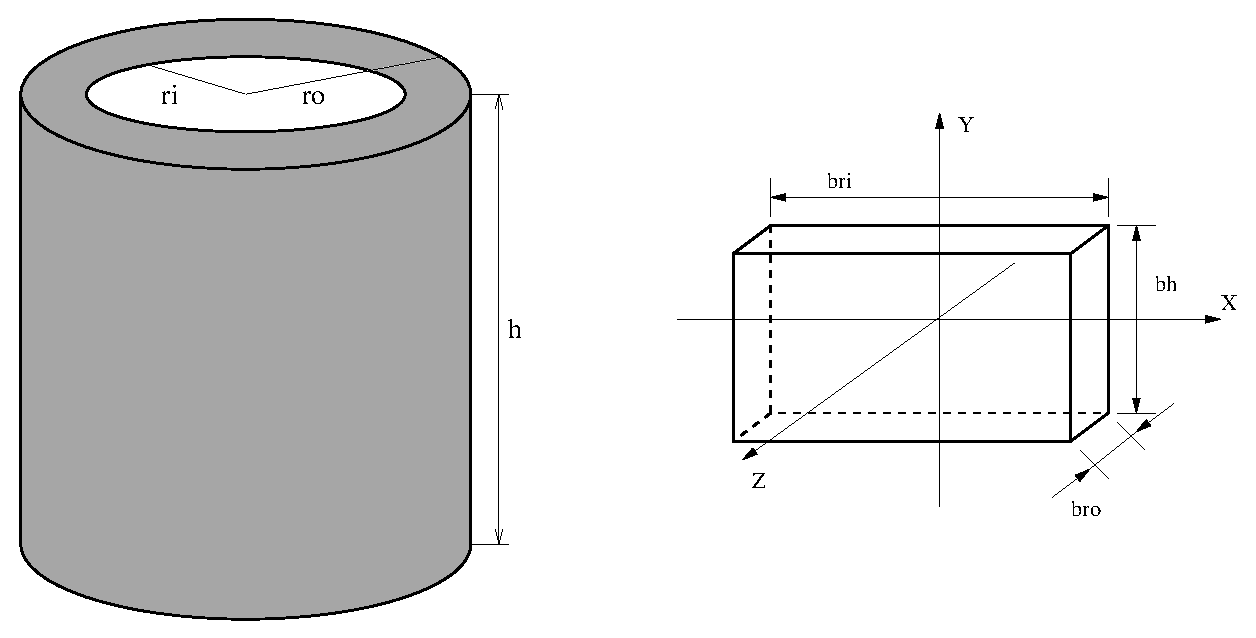
\includegraphics[width=0.9\textwidth]{figures/res_sample}
%    \caption{The two possible shapes of the \textbf{Res\_sample} component.}
%    \label{f:res_sample}
%  \end{center}
%\end{figure}
%
The component only propagates neutron rays that are scattered;
other rays are absorbed. The scattering probability is proportional to the neutron
flight path length inside the sample, to make a true volume weighting
of the sample. The reason for this is that the resolution
function of an instrument is independent of any sample properties
such as scattering and absorbtion cross sections but will in general
depend on sample size and shape.

The point of scattering inside the sample is chosen uniformly
along the neutron flight path inside the sample, and the scattered
neutron ray is given a random energy and direction. This energy is selected in
the interval $[E_0-\Delta E; E_0+\Delta E]$ which hence must be
chosen large enough to cover all interesting neutron energies.
Similarly, the scattered
direction is chosen in a user-specified range,
either within a sphere of radius $r_{\rm focus}$, within a rectangular
target with measures $(x_{\rm focus}, y_{\rm focus})$
or in the specified angular range. This target is positioned at the $x_{target}$, $y_{target}$, $z_{target}$ point in space, or using the target\_index for which e.g. 1 is the further component, -1 is the previous, etc...

A special feature, used when computing resolution functions, is that the
component stores complete information about the scattering event in the
output parameter \textit{res\_struct}. The information includes initial
and final wave vectors, the coordinates of the scattering point, and the
neutron weight after the scattering event. From this information the
scattering parameters $({\bf Q}, \omega)$ can be recorded
for every scattering event and used to compute the resolution function.
For an example of using the
information in the output parameter, see the description of the
\textbf{Res\_monitor} component in section~\ref{s:res_monitor}.



% Emacs settings: -*-mode: latex; TeX-master: "manual.tex"; -*-

\section{TOF\_Res\_sample: A sample-like component for TOF resolution calculation}
\label{s:tof_res_sample}

\component{TOF\_Res\_sample}{System}{$r_{\rm i}$, $r_{\rm o}$, $h$, $r_{\rm focus}$, $x_{\rm target}$, $y_{\rm target}$, $z_{\rm target}$, $t_0$, $\Delta t$ }{$x_w$, $y_h$, $z_t$, $x_{\rm focus}$, $y_{\rm focus}$, $a_{\rm v, focus}$, $a_{\rm h, focus}$, target index}{}

The component \textbf{TOF\_Res\_sample} scatters neutron rays isotropically
in position within a specified angular range. 
As for {\bf Res\_sample}, this component is meant
for computation of the resolution function, but in this case for one time bin in a
time-of-flight (TOF) instrument. The component selects uniformly the neutron 
energy so that neutron arrival time at the TOF detector lies within one time bin,
specified by $t_0$ and $\Delta t$.
For actual calculations of the resolution
function, {\bf TOF\_Res\_sample} should be used
together with \textbf{Res\_monitor}, described in
section~\ref{s:res_monitor}.

The shape of {\bf TOF\_Res\_sample} is either a hollow cylinder
or a rectangular box. 
The hollow cylinder shape is
specified with the inner and outer radius, $r_{\rm i}$ and $r_{\rm o}$,
respectively, and the height, $h$.
If these parameters are unspecified,
the shape is instead a box of dimensions $x_w$, $y_h$, and $z_t$.
%See figure~\ref{f:res_sample}.\par

The component only propagates neutron rays that are scattered; 
other rays are absorbed. 
As for {\bf Res\_sample}, the scattering probability is proportional to the neutron
flight path length inside the sample.
The point of scattering in the sample is chosen uniformly
along the neutron flight path inside the sample, and the scattered
direction is chosen in a user-specified range,
either within a sphere of radius $r_{\rm foc}$, within a rectangular
target with measures $(x_{\rm focus}, y_{\rm focus})$
or in the specified angular range. 
This target is positioned at the $x_{target}$, $y_{target}$, $z_{target}$ 
point in space, or using target\_index.

This component stores complete information about the scattering event in the
output parameter \textit{res\_struct}, see {\bf Res\_Sample}. 


\section{Res\_monitor: The monitor for resolution calculation}
\label{s:res_monitor}
\index{Monitors!Resolution monitor|see{Samples/Resolution function}}

%\component{Res\_monitor}{(System); Alan Tennant, HMI}{$x_{\rm min}$, $x_{\rm max}$, $y_{\rm min}$, $y_{\rm max}$, filename, res\_sample, buffer size}{$x_w$, $y_h$, $z_t$, options}{}
\mcdoccomp{misc/Res_monitor.parms}

The component {\bf Res\_monitor} is used for calculating the
resolution function of a particular instrument with detector of the
given shape, size, and position.
The shape of {\bf Res\_monitor} is by default rectangular,
but can be a box, a sphere, a disk, or a cylinder,
depending on the parameter ``options''.
The component works like a normal monitor, but
also records all scattering events and stores
them to a file that can later be read by 
the \MCS frontend tool \verb+mcresplot+.

For time-of-flight (TOF) instruments, {Res\_monitor} should be understood 
as giving the resolution of one time bin of the TOF-detector only; 
the bin properties being specified in the preceding {\bf TOF\_Res\_sample}.

As described in section~\ref{s:res_sample},
the {\bf Res\_monitor} should be used in connection with one of the
components {\bf Res\_sample} or {\bf TOF\_Res\_sample}, 
the name of which should be passed as an
input parameter to \textbf{Res\_monitor}. For example
\begin{lstlisting}
    COMPONENT mysample = Res_sample( ... )
    ...
    COMPONENT det = Res_monitor(res_sample_comp = mysample, ...)
    ...
\end{lstlisting}

The output file is in ASCII format, one line per scattering event, with
the following columns:
\begin{itemize}
\item ${\bf k}_{\rm i}$, the three components of the initial wave vector.
\item ${\bf k}_{\rm f}$, the three components of the final wave vector.
\item ${\bf r}$, the three components of the position of the scattering
  event in the sample.
\item $p_{\rm i}$, the neutron weight just after the scattering event.
\item $p_{\rm f}$, the relative neutron weight adjustment from sample to
  detector (so the total weight in the detector is $p_{\rm i}p_{\rm f}$).
\end{itemize}
From ${\bf k}_{\rm i}$ and ${\bf k}_{\rm f}$, we may compute 
the scattering parameters 
$\kappa = {\bf k}_{\rm i} - {\bf k}_{\rm f}$ and 
$\hbar \omega = \hbar^2/(2 m_{\rm n})({\bf k}_{\rm i}^2 - {\bf k}_{\rm f}^2)$.
The vectors are given in the local coordinate system of the resolution
sample component. The wave vectors are in units of $\mbox{\AA}^{-1}$, the
energy transfer in meV.

The output parameters from {\bf Res\_monitor}
are the three count numbers, \textit{Nsum}, \textit{psum},
and \textit{p2sum}, and the handle \textit{file} of the output file.


\newpage
\section{Progress\_bar: Simulation progress and automatic saving}
\component{Progress\_bar}{System}{percent, flag\_save, profile}{}{}
\label{s:progress-bar}
\index{Simulation progress bar}

This component displays the simulation progress and status
but does not affect the neutron parameters.
The display is updated in regular intervals of the full simulation;
the default step size is 10 \%, but it may be changed using
the \verb+percent+ parameter (from 0 to 100).
The estimated computation time is displayed at the begining
and actual simulation time is shown at the end.

Additionally, setting the \verb+flag_save+ to 1 results in
a regular save of the data files during the simulation.
This means that is is possible to view the data before the end
of the computation, and have also a trace of it in case of
computer crash. The achieved percentage of the simulation is stored in these temporary
data files. Technically, this save is equivalent to sending regularly
a USR2 signal to the running simulation.

The optional 'profile' parameter, when set to a file name, will produce the number of statistical events reaching each component in the simulation. This may be used to identify positions where events are lost.

\section{Beam\_spy: A beam analyzer}
\component{Beam\_spy}{System}{}{}{should overlap previous component}
\index{Monitors!Beam analyzer}

This component is at the same time an Arm and a simple Monitor. It analyzes all neutrons reaching it, and computes statistics for the beam, as well as the intensity.

This component does not affect the neutron beam, and does not contain any propagation call. Thus it gets neutrons from the previous component in the instrument description, and should better be placed at the same position, with \verb+AT (0,0,0) RELATIVE PREVIOUS+.


\appendix
% Emacs settings: -*-mode: latex; TeX-master: "manual.tex"; -*-

\chapter{Libraries and conversion constants}
\label{c:kernelcalls}
\index{Library|textbf}
\index{Library!Shared|see{Library/Components/share}}
\index{Library!mcstas-r|see{Library/Run-time}}

The \MCS\ Library contains a number of built-in functions
and conversion constants which are useful when constructing
components. These are stored in the \verb+share+ directory of
the \verb+MCSTAS+ library. \index{Library!Components!share}
\index{Environment variable!MCSTAS}

Within these functions, the 'Run-time' part is available for all
component/instrument descriptions. The other parts
% (see table~\ref{t:comp-share})
are dynamic, that is they are not
pre-loaded, but only imported once when a component requests it
using the \verb+%include+ \MCS\ keyword. For instance, within a
component C code block, (usually SHARE or DECLARE):
\index{Keyword!\%include}
\begin{verbatim}
    %include "read_table-lib"
\end{verbatim}
will include the 'read\_table-lib.h' file, and the 'read\_table-lib.c'
(unless the \verb+--no-runtime+ option is used with \verb+mcstas+).
Similarly,
\begin{verbatim}
    %include "read_table-lib.h"
\end{verbatim}
will \emph{only} include the 'read\_table-lib.h'.
The library embedding is done only once for all components (like the
 SHARE section). \index{Keyword!SHARE} For an example
of implementation, see {\bf Res\_monitor}.

In this Appendix, we present a short list of both each of the library contents
and the run-time features.

\section{Run-time calls and functions (\texttt{mcstas-r})}
\label{s:calls:run-time}
\index{Library!Run-time|textbf}
\index{Library!mcstas-r|see{Library/Run-time}}
Here we list a number of preprogrammed macros
which may ease the task of writing component and instrument definitions.

\subsection{Neutron propagation}
\index{Library!Run-time!SCATTER}
\index{Library!Run-time!ABSORB}
\index{Library!Run-time!PROP\_Z0}
\index{Library!Run-time!PROP\_DT}
\index{Library!Run-time!PROP\_GRAV\_DT}
\index{Library!Run-time!ALLOW\_BACKPROP}
Propagation routines perform all necessary operations to transport neutron rays
from one point to an other. Except when using the special
\verb+ALLOW_BACKPROP;+ call prior to exectuting any \verb+PROP_*+ propagation,
the neutron rays which have negative propagation times are removed automatically.
\begin{itemize}
\item {\bf ABSORB}. This macro issues an order to the overall
  \MCS\ simulator to interrupt the simulation of the current neutron
  history and to start a new one.
\item {\bf PROP\_Z0}. Propagates the neutron to the $z=0$ plane,
  by adjusting $(x,y,z)$ and $t$ accordingly from knowledge of the
  neutron velocity $(vx,vy,vz)$.
  If the propagation time is negative, the neutron ray is absorbed, except if a \verb+ALLOW_BACKPROP;+ preceeds it.

  For components that are centered along the $z$-axis,
  use the \verb+_intersect+ functions to determine intersection time(s),
  and then a \verb+PROP_DT+ call.
\item {\bf PROP\_DT}$(dt)$. Propagates the neutron through the
  time interval $dt$, adjusting $(x,y,z)$ and $t$ accordingly
  from knowledge of the neutron velocity. This macro automatically calls PROP\_GRAV\_DT when the \verb+--gravitation+ option has been set for the whole simulation.
\item {\bf PROP\_GRAV\_DT}$(dt,Ax,Ay,Az)$. Like {\bf PROP\_DT}, but it also
  includes gravity using the acceleration $(Ax,Ay,Az)$. In addition
  to adjusting $(x,y,z)$ and $t$, also $(vx,vy,vz)$ is modified.
\item {\bf ALLOW\_BACKPROP}. Indicates that the next propagation routine
  will not remove the neutron ray, even if negative propagation times
  are found. Further propagations are not affected.\index{Removed neutron events}
\item {\bf SCATTER}. This macro is used to denote a scattering event
  inside a component.
%, see section~\ref{s:comp-trace}.
  It should be used e.g
  to indicate that a component has interacted with the neutron ray
  (e.g. scattered or detected).
  This does not affect the simulation (see, however, {\bf Beamstop}),
  and it is mainly used by the
  \verb+MCDISPLAY+ section and the \verb+GROUP+ modifier
%(see~\ref{s:trace} and \ref{s:comp-mcdisplay}).
  See also the SCATTERED variable (below).
  \index{Keyword!GROUP} \index{Keyword!MCDISPLAY} \index{Keyword!EXTEND}
\end{itemize}

\subsection{Coordinate and component variable retrieval}
\index{Library!Run-time!MC\_GETPAR}
\index{Library!Run-time!NAME\_CURRENT\_COMP}
\index{Library!Run-time!POS\_A\_CURRENT\_COMP}
\index{Library!Run-time!ROT\_A\_CURRENT\_COMP}
\index{Library!Run-time!POS\_A\_COMP}
\index{Library!Run-time!ROT\_A\_COMP}
\index{Library!Run-time!STORE\_NEUTRON}
\index{Library!Run-time!RESTORE\_NEUTRON}
\index{Library!Run-time!SCATTERED}
\begin{itemize}
\item {\bf MC\_GETPAR}$(comp, outpar)$. This may be used in e.g. the FINALLY section of an
  instrument definition to reference the output parameters of a
  component.
% See page~\pageref{mcgetpar} for details.
\item {\bf NAME\_CURRENT\_COMP} gives the name of the current component as a string.
\item {\bf POS\_A\_CURRENT\_COMP} gives the absolute position of the
  current component. A component of the vector is referred to as
  POS\_A\_CURRENT\_COMP.$i$ where $i$ is $x$, $y$ or $z$.
\item {\bf ROT\_A\_CURRENT\_COMP} and
  {\bf ROT\_R\_CURRENT\_COMP} give the orientation
  of the current component as rotation matrices
  (absolute orientation and the orientation relative to
  the previous component, respectively). A
  component of a rotation matrix is referred to as
  ROT\_A\_CURRENT\_COMP$[m][n]$, where $m$ and
  $n$ are 0, 1, or 2 standing for $x,y$ and $z$ coordinates respectively.
\item {\bf POS\_A\_COMP}$(comp)$ gives the absolute position
  of the component with the name {\em comp}. Note that
  {\em comp} is not given as a string. A component of the
  vector is referred to as POS\_A\_COMP$(comp).i$
  where $i$ is $x$, $y$ or $z$.
\item {\bf ROT\_A\_COMP}$(comp)$ and
  {\bf ROT\_R\_COMP}$(comp)$ give the orientation of the
  component {\em comp} as rotation matrices (absolute
  orientation and the orientation relative to its
  previous component, respectively). Note that {\em comp}
  is not given as a string. A component of  a rotation
  matrice is referred to as
  ROT\_A\_COMP$(comp)[m][n]$, where $m$ and $n$ are
  0, 1, or 2.
\item {\bf INDEX\_CURRENT\_COMP} is the number (index) of the
       current component  (starting from 1).
\item {\bf POS\_A\_COMP\_INDEX}$(index)$ is the absolute position of
  component $index$. \\
  POS\_A\_COMP\_INDEX (INDEX\_CURRENT\_COMP) is the same as \\
  POS\_A\_CURRENT\_COMP. You may use \\
  POS\_A\_COMP\_INDEX  (INDEX\_CURRENT\_COMP+1) \\
  to make, for instance, your
  component access the position of the next component (this is usefull for
  automatic targeting).  A component of the vector is referred to as
  POS\_A\_COMP\_INDEX$(index).i$ where $i$ is $x$, $y$ or $z$.
\item {\bf POS\_R\_COMP\_INDEX} works the same as above,
  but with relative coordinates.
\item {\bf STORE\_NEUTRON}$(index, x, y, z, vx, vy, vz, t$, $sx, sy,
sz, p)$ stores the current neutron state in the trace-history table,
in local coordinate system. $index$ is usually INDEX\_CURRENT\_COMP.
This is automatically done when entering each component of an
instrument.
\item {\bf RESTORE\_NEUTRON}$(index, x, y, z, vx, vy, vz, t, sx, sy,
sz, p)$ restores the neutron state to the one at the input of the
component $index$. To ignore a component effect, use
RESTORE\_NEUTRON (INDEX\_CURRENT\_COMP, \\
$x, y, z, vx, vy, vz, t,
sx, sy, sz, p$) at the end of its TRACE section, or in its EXTEND
section. These neutron states are in the local component coordinate
systems.
\item {\bf SCATTERED} is a variable set to 0 when entering
  a component, which is incremented each time a SCATTER event occurs.
  This may be used in the \verb+EXTEND+ sections to determine whether
  the component interacted with the current neutron ray.
\item {\bf extend\_list}($n$, \&\textit{arr}, \&\textit{len},
  \textit{elemsize}). Given an array \textit{arr} with \textit{len}
  elements each of size \textit{elemsize}, make sure that the array is
  big enough to hold at least $n$ elements, by extending \textit{arr}
  and \textit{len} if necessary. Typically used when reading a list of
  numbers from a data file when the length of the file is not known in advance.
\item {\bf mcset\_ncount}$(n)$. Sets the number of neutron histories to simulate to $n$.
\item {\bf mcget\_ncount}(). Returns the number of neutron histories to simulate (usually set by option \verb+-n+).
\item {\bf mcget\_run\_num}(). Returns the number of neutron histories that have been simulated until now.
\end{itemize}

\subsection{Coordinate transformations}
\begin{itemize}
\item {\bf coords\_set}$(x,y,z)$ returns a Coord structure (like POS\_A\_CURRENT\_COMP) with $x$, $y$ and $z$ members.
\item {\bf  coords\_get}$(P,$ \&$x$, \&$y$, \&$z)$ copies the $x$, $y$ and
$z$ members of the Coord structure $P$ into $x,y,z$ variables.
\item {\bf coords\_add}$(a,b)$, {\bf coords\_sub}$(a,b)$, {\bf
coords\_neg}$(a)$ enable to  operate on coordinates, and return the
resulting Coord structure.
\item {\bf rot\_set\_rotation}({\it Rotation t}, $\phi_x, \phi_y, \phi_z$)
  Get transformation matrix for rotation
  first $\phi_x$ around x axis, then $\phi_y$ around y,
  and last $\phi_z$ around z. $t$ should be a 'Rotation' ([3][3] 'double' matrix).
\item {\bf rot\_mul}{\it (Rotation t1, Rotation t2, Rotation t3)} performs $t3 = t1 . t2$.
\item {\bf rot\_copy}{\it (Rotation dest, Rotation src)} performs $dest = src$ for Rotation arrays.
\item {\bf rot\_transpose}{\it (Rotation src, Rotation dest)} performs $dest = src^t$.
\item {\bf rot\_apply}{\it (Rotation t, Coords a)} returns a Coord structure which is $t.a$
\end{itemize}

\subsection{Mathematical routines}
\begin{itemize}
\item {\bf NORM}$(x,y,z)$. Normalizes the vector $(x,y,z)$ to have
  length 1.
\item {\bf scalar\_prod}$(a_x,a_y,a_z,b_x,b_y,b_z)$. Returns the scalar
  product of the two vectors $(a_x,a_y,a_z)$ and $(b_x,b_y,b_z)$.
\item {\bf vec\_prod}(\&$a_x$,\&$a_y$,\&$a_z$,$b_x$,$b_y$,$b_z$, $c_x$,$c_y$,$c_z$). Sets
  $(a_x,a_y,a_z)$ equal to the vector product $(b_x,b_y,b_z) \times (c_x,c_y,c_z)$.
\item {\bf rotate}(\&$x$,\&$y$,\&$z$,$v_x$,$v_y$,$v_z$,$\varphi$,$a_x$,$a_y$,$a_z$). Set
  $(x,y,z)$ to the result of rotating the vector $(v_x,v_y,v_z)$
  the angle $\varphi$ (in radians) around the vector $(a_x,a_y,a_z)$.
\item {\bf normal\_vec}(\&$n_x$, \&$n_y$, \&$n_z$, $x$, $y$, $z$).
  Computes a unit vector $(n_x, n_y, n_z)$ normal to the vector
  $(x,y,z)$.
\item {\bf solve\_2nd\_order}(*$t$, $A$,  $B$,  $C$).
  Solves the 2$^{nd}$ order equation $At^2 + Bt + C = 0$ and returns
  the smallest positive solution into pointer *$t$.
\end{itemize}

\subsection{Output from detectors}
Details about using these functions are given in the \MCS\ User Manual.
\begin{itemize}
\item {\bf DETECTOR\_OUT\_0D}$(...)$. Used to output the results from a
  single detector. The name of the detector is output together
  with the simulated intensity and estimated statistical error. The
  output is produced in a format that can be read by \MCS\ front-end
  programs.
%See section~\ref{s:comp-finally} ??? for details.
\item {\bf DETECTOR\_OUT\_1D}$(...)$. Used to output the results from a
  one-dimensional detector. Integrated intensities error etc. is also
  reported as for DETECTOR\_OUT\_0D.
%See section~\ref{s:comp-finally} for details.
\item {\bf DETECTOR\_OUT\_2D}$(...)$. Used to output the results from a
  two-dimentional detector. Integrated intensities error etc. is also
  reported as for DETECTOR\_OUT\_0D.
%See section~\ref{s:comp-finally} for details.
\item {\bf DETECTOR\_OUT\_3D}$(...)$. Used to output
  the results from a three-dimentional detector. Arguments are the same as
  in DETECTOR\_OUT\_2D, but with an additional $z$ axis.
  Resulting data files are treated as 2D data, but the 3rd dimension is
  specified in the $type$ field. Integrated intensities error etc. is also
  reported as for DETECTOR\_OUT\_0D.
\item {\bf mcinfo\_simulation}{\it (FILE *f, mcformat,
  char *pre, char *name)} is used to append the simulation parameters into file $f$
  (see for instance {\bf Res\_monitor}).
  Internal variable $mcformat$ should be used as specified.
  Please contact the authors for further information.
\end{itemize}

\subsection{Ray-geometry intersections}
\begin{itemize}
\item {\bf inside\_rectangle}(\&$x$, \&$y$, $x$, $xw$, $yh$).
  Return 1 if $-xw/2 \leq x \leq xw/2$ AND $-yh/2 \leq y \leq yh/2$.
  Else return 0.
\item {\bf box\_intersect}(\&$t_1$, \&$t_2$, $x$, $y$, $z$, $v_x$, $v_y$, $v_z$,
  $d_x$, $d_y$, $d_z$). Calculates the (0, 1, or 2) intersections between
  the neutron path and a box of dimensions $d_x$, $d_y$, and $d_z$,
  centered at the origin for a neutron with the parameters
  $(x,y,z,v_x,v_y,v_z)$. The times of intersection are returned
  in the variables $t_1$ and $t_2$, with $t_1 < t_2$. In the case
  of less than two intersections, $t_1$ (and possibly $t_2$) are set to
  zero. The function returns true if the neutron intersects the box,
  false otherwise.
\item {\bf cylinder\_intersect}(\&$t_1$, \&$t_2$, $x$, $y$, $z$, $v_x$, $v_y$, $v_z$,
  $r$, $h$).  Similar to {\bf box\_intersect}, but using a cylinder of height $h$ and radius $r$,
  centered at the origin.
\item {\bf sphere\_intersect}(\&$t_1$, \&$t_2$, $x$, $y$, $z$, $v_x$, $v_y$, $v_z$,
  $r$). Similar to {\bf box\_intersect}, but using a sphere
  of radius $r$.
\end{itemize}

\subsection{Random numbers}
\begin{itemize}
\item {\bf rand01}(). Returns a random number distributed uniformly between 0 and 1.
\item {\bf randnorm}(). Returns a random number from a normal
  distribution centered around 0 and with $\sigma=1$. The algorithm used to
  sample the normal distribution is explained in Ref.~\cite[ch.7]{num_rep}.
\item {\bf randpm1}(). Returns a random number distributed uniformly between -1 and 1.
\item {\bf randtriangle}(). Returns a random number from a triangular distribution between -1 and 1.
\item {\bf randvec\_target\_circle}(\&$v_x$, \&$v_y$, \&$v_z$, \&$d\Omega$,
  aim$_x$, aim$_y$, aim$_z$, $r_f$). Generates a random vector $(v_x, v_y,
  v_z)$, of the same length as (aim$_x$, aim$_y$, aim$_z$), which is
  targeted at a \emph{disk} centered at (aim$_x$, aim$_y$, aim$_z$) with
  radius $r_f$ (in meters), and perpendicular to the \emph{aim} vector.. All directions
  that intersect the circle are chosen with equal probability. The solid
  angle of the circle as seen from the position of the neutron is returned
  in $d\Omega$. This routine was previously called {\bf randvec\_target\_sphere}
  (which still works).
\item {\bf randvec\_target\_rect\_angular}(\&$v_x$, \&$v_y$, \&$v_z$,
  \&$d\Omega$, aim$_x$, aim$_y$, aim$_z$,$h, w, Rot$) does the same as
  randvec\_target\_circle but targetting at a rectangle with angular dimensions
  $h$ and $w$ (in {\bf radians}, not in degrees as other angles). The
  rotation matrix $Rot$ is the coordinate system orientation in the absolute
  frame, usually ROT\_A\_CURRENT\_COMP.
\item {\bf randvec\_target\_rect}(\&$v_x$, \&$v_y$, \&$v_z$,
  \&$d\Omega$, aim$_x$, aim$_y$, aim$_z$,$height, width, Rot$) is the same as
  randvec\_target\_rect\_angular but $height$ and $width$ dimensions are given
  in meters. This function is useful to e.g. target at a guide entry window
  or analyzer blade.
\end{itemize}

\section{Reading a data file into a vector/matrix (Table input, \texttt{read\_table-lib})}
\label{s:read-table}
\index{Library!read\_table-lib (Read\_Table)|textbf}
  The \verb+read_table-lib+ provides functionalities for reading text
  (and binary) data files. To use this library,
  add a \verb+%include "read_table-lib"+ in your component definition
  DECLARE or SHARE section. Tables are structures of type \verb+t_Table+
  (see \verb+read_table-lib.h+ file for details):
\begin{verbatim}
    /* t_Table structure (most important members) */
    double *data;     /* Use Table_Index(Table, i j) to extract [i,j] element */
    long    rows;     /* number of rows */
    long    columns;  /* number of columns */
    char   *header;   /* the header with comments */
    char   *filename; /* file name or title */
    double  min_x;    /* minimum value of 1st column/vector */
    double  max_x;    /* maximum value of 1st column/vector */
\end{verbatim}

Available functions to read \emph{a single} vector/matrix are:
\begin{itemize}
\item {\bf Table\_Init}(\&$Table$, $rows$, $columns$) returns an allocated
  Table structure. Use $rows=columns=0$ not to allocate memory and return an empty table.
  Calls to Table\_Init are \emph{optional}, since initialization is being
  performed by other functions already.
\item {\bf Table\_Read}(\&$Table$, $filename$, $block$)
  reads numerical block number
  $block$ (0 to concatenate all) data from \emph{text} file $filename$ into $Table$,
  which is as well initialized in the process.
  The block number changes when the numerical data changes its size,
  or a comment is encoutered (lines starting
  by '\verb+# ; % /+'). If the data could not be read,
  then $Table.data$ is NULL and $Table.rows = 0$.
  You may then try to read it using Table\_Read\_Offset\_Binary.
  Return value is the number of elements read.
\item {\bf Table\_Read\_Offset}(\&$Table$, $filename$, $block$, \&\textit{offset}, $n_{rows}$)
  does the same as Table\_Read except that it starts at offset \textit{offset}
  (0 means begining of file) and reads $n_{rows}$ lines (0 for all).
  The \textit{offset} is returned as the final offset reached after
  reading the $n_{rows}$ lines.
\item {\bf Table\_Read\_Offset\_Binary}(\&$Table$, $filename$, $type$,
  $block$, \&\textit{offset}, $n_{rows}$, $n_{columns}$) does the same as
  Table\_Read\_Offset, but also specifies the $type$ of the file (may
  be "float" or "double"), the number $n_{rows}$ of rows to read, each
  of them having $n_{columns}$ elements. No text header should be present
  in the file.
\item {\bf Table\_Rebin}(\&$Table$) rebins all $Table$ rows with increasing, evenly spaced first column (index 0), e.g. before using Table\_Value. Linear interpolation is performed for all other columns. The number of bins for the rebinned table is determined from the smallest first column step.
\item {\bf Table\_Info}$(Table)$ print information about the table $Table$.
\item {\bf Table\_Index}($Table, m, n$) reads the $Table[m][n]$ element.
\item {\bf Table\_Value}($Table, x, n$) looks for the closest $x$
  value in the first column (index 0), and extracts in this row the
  $n$-th element (starting from 0). The first column is thus the 'x' axis for the data.
\item {\bf Table\_Free}(\&$Table$) free allocated memory blocks.
\item {\bf Table\_Value2d}($Table$, $X$, $Y$) Uses 2D linear interpolation on a Table, from (X,Y) coordinates and returns the corresponding value.
\end{itemize}

Available functions to read \emph{an array} of vectors/matrices in a \emph{text} file are:
\begin{itemize}
\item {\bf Table\_Read\_Array}($File$, \&$n$) read and split $file$
into as many blocks as necessary and return a \verb+t_Table+ array.
Each block contains a single vector/matrix. This only works for text files.
The number of blocks is put into $n$.
\item {\bf Table\_Free\_Array}(\&$Table$) free the $Table$ array.
\item {\bf Table\_Info\_Array}(\&$Table$) display information about all data blocks.
\end{itemize}

The format of text files is free. Lines starting by '\verb+# ; % /+' characters are considered to be comments, and stored in $Table.header$. Data blocks are vectors and matrices. Block numbers are counted starting from 1, and changing when a comment is found, or the column number changes. For instance, the file 'MCSTAS/data/BeO.trm' (Transmission of a Berylium filter) looks like:
\begin{verbatim}
  # BeO transmission, as measured on IN12
  # Thickness: 0.05 [m]
  # [ k(Angs-1) Transmission (0-1) ]
  # wavevector multiply
  1.0500  0.74441
  1.0750  0.76727
  1.1000  0.80680
  ...
\end{verbatim}
Binary files should be of type "float" (i.e. REAL*32) and "double" (i.e. REAL*64),
and should \emph{not} contain text header lines. These files are platform
dependent (little or big endian).

The $filename$ is first searched into the current directory (and all user additional locations specified using the \verb+-I+ option, see the 'Running \MCS\ ' chapter in the User Manual), and if not found, in the \verb+data+ sub-directory of the \verb+MCSTAS+ library location. \index{Library!Components!data}
\index{Environment variable!MCSTAS} This way, you do not need to have local copies of the \MCS\ Library Data files (see table~\ref{t:comp-data}).

A usage example for this library part may be:
\begin{verbatim}
  t_Table Table;       // declare a t_Table structure
  char file[]="BeO.trm";  // a file name
  double x,y;

  Table_Read(&Table, file, 1);  // initialize and read the first numerical block
  Table_Info(Table);            // display table informations
  ...
  x = Table_Index(Table, 2,5);  // read the 3rd row, 6th column element
                                // of the table. Indexes start at zero in C.
  y = Table_Value(Table, 1.45,1);  // look for value 1.45 in 1st column (x axis)
                                // and extract 2nd column value of that row
  Table_Free(&Table);           // free allocated memory for table
\end{verbatim}
Additionally, if the block number (3rd) argument of  {\bf Table\_Read} is 0, all blocks will be concatenated.
The {\bf Table\_Value} function assumes that the 'x' axis is the first column (index 0).
Other functions are used the same way with a few additional parameters, e.g. specifying an offset for reading files, or reading binary data.

This other example for text files shows how to read many data blocks:
\begin{verbatim}
  t_Table *Table;       // declare a t_Table structure array
  long     n;
  double y;

  Table = Table_Read_Array("file.dat", &n); // initialize and read the all numerical block
  n = Table_Info_Array(Table);     // display informations for all blocks (also returns n)

  y = Table_Index(Table[0], 2,5);  // read in 1st block the 3rd row, 6th column element
                                   // ONLY use Table[i] with i < n !
  Table_Free_Array(Table);         // free allocated memory for Table
\end{verbatim}

You may look into, for instance, the source files for
{\bf Monochromator\_curved} or {\bf Virtual\_input}
for other implementation examples.

\section{Monitor\_nD Library}
\index{Library!monitor\_nd-lib}

This library gathers a few functions used by a set of monitors e.g. Monitor\_nD, Res\_monitor, Virtual\_output, etc.
It may monitor any kind of data, create the data files, and may display many geometries (for \verb+mcdisplay+).
Refer to these components for implementation examples, and ask the authors for more details.

\section{Adaptive importance sampling Library}
\index{Library!adapt\_tree-lib}

This library is currently only used by the components {\bf Source\_adapt}
and {\bf Adapt\_check}. It performs adaptive importance sampling of neutrons for simulation efficiency optimization.
Refer to these components for implementation examples, and ask the authors for more details.

\section{Vitess import/export Library}
\index{Library!vitess-lib}

This library is used by the components
{\bf Vitess\_input} and {\bf Vitess\_output},
as well as the \verb+mcstas2vitess+ utility.
% (see section~\ref{s:mcstas2vitess}).
\index{Tools!mcstas2vitess}
Refer to these components for implementation examples, and ask the authors for more details.

\section{Constants for unit conversion etc.}
The following predefined constants are useful for conversion
between units
\def\textvb{\textbf}
\begin{center}
\begin{tabular}{|l|c|p{0.29\textwidth}|p{0.252\textwidth}|}
\hline
Name & Value & Conversion from & Conversion to \\ \hline
\textvb{DEG2RAD} & $2 \pi / 360$ & Degrees & Radians \\
\textvb{RAD2DEG} & $360 / (2 \pi)$ & Radians & Degrees \\
\textvb{MIN2RAD} & $2 \pi / (360 \cdot 60)$
  & Minutes of arc & Radians \\
\textvb{RAD2MIN} & $(360\cdot 60) / (2 \pi)$
  & Radians & Minutes of arc \\
\textvb{V2K} & $10^{10} \cdot m_{\rm N}/\hbar$
  & Velocity (m/s) & {\bf k}-vector (\AA$^{-1}$) \\
\textvb{K2V} & $10^{-10} \cdot \hbar / m_{\rm N}$
  & {\bf k}-vector (\AA$^{-1}$) & Velocity (m/s) \\
\textvb{VS2E} & $m_{\rm N} / (2 e)$
  & Velocity squared (m$^2$ s$^{-2}$) & Neutron energy (meV) \\
\textvb{SE2V} & $\sqrt{2 e/m_{\rm N}}$
  & Square root of neutron energy (meV$^{1/2}$) & Velocity (m/s) \\
\textvb{FWHM2RMS} & $1/\sqrt{8\log(2)}$
  & Full width half maximum & Root mean square (standard deviation) \\
\textvb{RMS2FWHM} & $\sqrt{8\log(2)}$
  & Root mean square (standard deviation) & Full width half maximum \\
\textvb{MNEUTRON} & $1.67492 \cdot 10^{-27}$~kg
  & Neutron mass, $m_{\rm n}$ & \\
\textvb{HBAR} & $1.05459 \cdot 10^{-34}$~Js
  & Planck constant, $\hbar$ & \\
\textvb{PI} & $3.14159265...$
  & $\pi$ & \\
\textvb{FLT\_MAX} & 3.40282347E+38F
  & a big float value & \\
\hline
\end{tabular}
\end{center}
 % as in manual
% Emacs settings: -*-mode: latex; TeX-master: "manual.tex"; -*-

\chapter{The \MCS terminology}
\label{s:terminology}

This is a short explanation of phrases and terms which have a specific
meaning within \MCS. We have tried to keep the list as short
as possible with the risk that the reader may occasionally miss
an explanation. In this case, you are more than welcome to contact
the \MCS core team.

\noindent
\begin{itemize}
\item\textbf{Arm}  A generic \MCS component which defines a frame of reference
      for other components.\index{Arm|textit}
\item\textbf{Component} One unit ({\em e.g.} optical element) in a neutron
      spectrometer. These are considered as Types of elements to be instantiated in an Instrument description.\index{Component|textit}
\item\textbf{Component instance} A named Component (of a given Type) inserted in an Instrument description.\index{Component!instance|textit}
\item\textbf{Definition parameter} An input parameter for a component. For
  example the radius of a sample component or the divergence of a collimator.\index{Definition parameter|textit}
\item\textbf{Input parameter} For a component, either a definition parameter
or a setting parameter. These parameters are supplied by the user to
define the characteristics of the particular instance of the component
definition. For an instrument, a parameter that can be changed at
simulation run-time.\index{Input parameter|textit}
\item\textbf{Instrument} An assembly of \MCS components defining
      a neutron spectrometer.\index{Instrument|textit}
\item\textbf{Kernel} The \MCS meta-language definition and the associated compiler \mcs.\index{Kernel|textit}
\item\textbf{\MCS} Monte Carlo Simulation of Triple Axis Spectrometers
       (the name of this package).
  Pronunciation ranges from \emph{mex-tas}, to \emph{mac-stas} and \emph{m-c-stas}.\index{McStas!name}\index{McStas!pronunciation}
\item\textbf{Output parameter} An output parameter for a component.
  For example the counts in a monitor. An output parameter may be
  accessed from the instrument in which the component is used using
  \verb`MC_GETPAR`.\index{Output parameter|textit}
\item\textbf{Run-time} C code, contained in the files
  \verb+mcstas-r.c+ and \verb+mcstas-r.h+ included in the \MCS
  distribution, that declare functions and variables used by the
  generated simulations.\index{Run-time|textit}
\item\textbf{Setting parameter} Similar to a definition parameter, but with the
  restriction that the value of the parameter must be a number.\index{Setting parameter|textit}
\end{itemize}
       % as in manual

\addcontentsline{toc}{chapter}{\protect\numberline{}{Bibliography}}
\bibliography{mcstas}
\bibliographystyle{jacs}

\addcontentsline{toc}{chapter}{\protect\numberline{}{Index and keywords}}
\printindex
\newcommand{\titel}[1]{{\egtrm Title and author(s)}
 \rm\\[3dd]#1\\[\baselineskip]}
\newcommand{\forfatter}[1]{{\egtrm}
 \rm #1\\\underline{\makebox[\textwidth]{\mbox{}}}\\[-3dd]}
\newcommand{\isbn}[1]{\parbox[t]{0.75\textwidth}{{\footnotesize ISBN}
 \normalsize\rm\\[3dd]#1\mbox{}}}
\newcommand{\issn}[1]{\parbox[t]{0.25\textwidth}{{\footnotesize ISSN}
 \normalsize\rm\\[3dd] #1\mbox{}}\\[0.5\baselineskip]
 \underline{\makebox[\textwidth]{\mbox{}}}\\[-3dd]}
\newcommand{\afdeling}[1]{\parbox[t]{0.75\textwidth}{{\egtrm Dept. or group}
 \rm\\[3dd]#1\mbox{}}}
\newcommand{\dato}[1]{\parbox[t]{0.25\textwidth}{{\egtrm Date}
 \rm\\[3dd] #1\mbox{}}\\[0.5\baselineskip]
 \underline{\makebox[\textwidth]{\mbox{}}}\\[-3dd]}
\newcommand{\regnummer}[1]{\parbox[t]{0.5\textwidth}{{\egtrm
 Groups own reg. number(s)}\rm\\[3dd] #1\mbox{}}}
\newcommand{\projektnummer}[1]{\parbox[t]{0.5\textwidth}{{\egtrm
 Project/contract No.}\rm\\[3dd] #1\mbox{}}\\[0.5\baselineskip]
 \underline{\makebox[\textwidth]{\mbox{}}}\\[-3dd]}
\newcommand{\sider}[1]{\parbox[t]{0.25\textwidth}{{\egtrm Pages}
 \rm\\[3dd]\mbox{}#1\mbox{}}}
\newcommand{\tabeller}[1]{\parbox[t]{0.25\textwidth}{{\egtrm Tables}
 \rm\\[3dd]\mbox{}#1\mbox{}}}
\newcommand{\figurer}[1]{\parbox[t]{0.25\textwidth}{{\egtrm Illustrations}
 \rm\\[3dd]\mbox{}#1\mbox{}}}
\newcommand{\referencer}[1]{\parbox[t]{0.25\textwidth}{{\egtrm References}
 \rm\\[3dd]\mbox{}#1\mbox{}}\\[0.5\baselineskip]
 \underline{\makebox[\textwidth]{\mbox{}}}\\[-3dd]}
\newcommand{\resume}[1]{{\egtrm Abstract (Max. 2000 char.)}
 \rm\\[3dd]#1\mbox{}\\\underline{\makebox[\textwidth]{\mbox{}}}\\[-3dd]}
\newcommand{\deskriptorer}[1]{{\egtrm Descriptors}
 \rm\\[3dd]#1\mbox{}\\
 \underline{\makebox[\textwidth]{\mbox{}}}\\[-3dd]}
\newenvironment{datablad}{\parindent 0pt\parskip 0pt\clearpage
 \frenchspacing\thispagestyle{empty}\normalsize
 \underline{\makebox[\textwidth]{\bf Bibliographic Data Sheet
 \rule[-6dd]{0cc}{1cc}\hfill\reportnum \reportlan}}\\}{

\footnotesize\vspace{-\baselineskip}
Available on request from:\\
Information Service Department, Ris{\o} DTU\\
(Afdelingen for Informationsservice, Ris{\o} DTU) \\
P.O. Box 49, DK--4000 Roskilde, Denmark \\
Phone +45 4677 4004,
Telefax +45 4677 4013
\clearpage}

\def\reportlan{}
% Ensure datablad is on a left-hand page.
\newpage\ifodd\csname c@page\endcsname\noindent\hbox{}\par\newpage\else\fi
\begin{datablad}
\titel{Component Manual to the Neutron Ray-Tracing Package
 \MCS , Version \version}
\forfatter{Peter Kj\ae r Willendrup, Erik Knudsen, Kim Lefmann and Emmanuel Farhi}
\isbn{ISBN 978--87--550--3680--2}\issn{0106--2840}
\afdeling{Materials Research Department}
\dato{\reldate}
\regnummer{---}
\projektnummer{---}
\sider{\thepage}\tabeller{2}\figurer{15}\referencer{10}
\resume{The software package McStas is a tool for carrying out Monte Carlo
ray-tracing simulations of neutron scattering instruments with high
complexity and precision. The simulations can compute all aspects of the
performance of instruments and can thus be used to optimize the use of
existing equipment, design new instrumentation, and carry out virtual
experiments for e.g. training, experimental planning or data analysis. McStas
is based on a unique design where an automatic compilation process
translates high-level textual instrument descriptions into efficient
ANSI-C code. This design makes it simple to set up typical simulations
and also gives essentially unlimited freedom to handle more unusual
cases.

This report constitutes the reference manual for McStas, and,
together with the manual for the McStas components, it
contains documentation of most aspects of the program. It covers
the various ways to compile and run simulations, a description of the
meta-language used to define simulations, 
%a full description of all
%algorithms used to calculate the effects of the various optical
%components in instruments, 
and some example simulations performed with
the program.
}
\deskriptorer{Neutron Instrumentation; Monte Carlo Simulation; Software}
\end{datablad}



\end{document}
